% main.tex -- main text of the article; the Supplementary Material is supplement.tex (same macros).
% Build: sh build_pdfs.sh  (the two documents cite each other through xr-hyper, using copies of their .aux files
%   in xref/; reproduce.md describes the sequence)
% Rule:   every number carries a comment  % src: <path of the result file or script it comes from>;
%         paths are relative to the root of the repository (see README.md).
\documentclass[11pt,a4paper]{article}

\usepackage[T1]{fontenc}
\usepackage[utf8]{inputenc}
\usepackage{lmodern}
\usepackage[a4paper,margin=2.5cm]{geometry}
\usepackage{amsmath,amssymb,amsthm}
\usepackage{graphicx}
\usepackage{booktabs}
\usepackage{array}
\usepackage{longtable}
\usepackage[section]{placeins}   % keeps every figure and table inside its own section
\usepackage{microtype}
\usepackage{xcolor}
\usepackage[round]{natbib}
\usepackage{xr-hyper}
\usepackage[colorlinks=true,linkcolor=blue!50!black,citecolor=blue!50!black,urlcolor=blue!50!black]{hyperref}
\externaldocument{xref/supplement}[supplement.pdf]

% float placement: let a large table or figure share a page with text instead of drifting to the end of its section
\renewcommand{\topfraction}{0.9}
\renewcommand{\bottomfraction}{0.8}
\renewcommand{\textfraction}{0.08}
\renewcommand{\floatpagefraction}{0.75}
\setcounter{topnumber}{3}
\setcounter{bottomnumber}{2}
\setcounter{totalnumber}{4}

\graphicspath{{figures/}}
% macros.tex -- notation and theorem environments of the article and its Supplementary Material.
% Loaded by main.tex and supplement.tex after the packages.  One symbol per quantity; symbols that are used in
% a single section of the Supplementary Material only are defined at the top of that section.
%
% =====================================================================================
% NOTATION TABLE (single source of truth)
% -------------------------------------------------------------------------------------
% CONVENTIONS
%   * Sites are ZERO-BASED: \Om = {0,...,N-1}^d.  Corner start \vo = (0,...,0), opposite
%     corner target \va = (N-1,...,N-1) in the corner-to-corner (CC) geometry.
%     (Every formula of the article is stated zero-based and was checked numerically in that
%     form: code/article/closed_form_checks.py, appA_proofs_check.py.)
%   * Time is measured in steps of the discrete-time walk.  "Unit rate" means the
%     continuous-time walk with total jump rate 1 (equivalently q = 1 in q*t).
%   * s WITHOUT subscript is always the Laplace variable; s_k WITH an integer subscript
%     is always sin(pi k / 2N).  The start site is \vo (never "s").
%   * ln is the natural logarithm.
%
% MODEL
%   \dd            d            dimension (1, 2, 3)
%   N              N            number of sites per side
%   \Om            \Omega       lattice {0,...,N-1}^d
%   \nn            n            number of accessible sites (N^d on the clean lattice; |\Cset| with defects)
%   q              q            activity: probability of attempting a move in one step, 0 < q <= 1
%   \vo, \va, \vx  o, a, x      start site, target site, generic site (bold); components o_i, a_i, x_i
%   \Pm            P            transition matrix of the reflecting (cancelled-move) walk; \Pm_1 its q = 1 version
%   \Qm            Q            P with the row and column of the target removed (killed chain)
%   \Lm            L            I - P;   \Lp = L^+  its Moore-Penrose pseudo-inverse
%   \Glap          G            pseudo-inverse of the unit-conductance graph Laplacian (I - P = (q/2d) * Laplacian)
%   \Reff          R            effective resistance (unit resistors);  R_N: opposite corners of the N x N grid
%
% FIRST-PASSAGE QUANTITIES
%   \FPT           \mathcal{T}  random first-passage (hitting) time of the target
%   \Sv(t)         S(t)         survival probability  P(\FPT > t)
%   \pmf(t)        f(t)         first-passage probability mass function  P(\FPT = t) = S(t-1) - S(t)
%   \gd(t)         g(t)         first-passage density of the continuous-time walk (unit rate unless stated)
%   \MF            T            mean first-passage time (MFPT), in steps;  T_{\vo\to\va} when the pair matters
%   \TN            T_N          corner-to-corner MFPT for d = 2;   \TNd{d}  T_N^{(d)} in dimension d
%   \tmode         t^*          mode (most probable first-passage time): smallest argmax_t f(t)
%   \tmodec        t^*_c        mode of the continuous-time density at unit rate (at activity q the mode is t^*_c / q)
%   \tcert         t_cert       time beyond which the PMF is certified to stay below its maximum (Prop. s3_methods:prop-certificate)
%   X_t                         position of the walker after t steps;  h: vector of the mean first-passage times over the start sites
%   \ratio         \varrho      mode-to-mean ratio  t^*/T
%   \Ftil(z)       \widetilde F(z)   probability generating function  sum_t f(t) z^t
%   \Fhat(s)       \widehat F(s)     Laplace transform of g;   \Ptil, \Phat: propagator transforms
%   \hone(m,m')    h_1(m,m')    hitting time from m to m' of the one-dimensional chain with q = 1
%
% SPECTRAL NOTATION
%   \angk{k}       \vartheta_k     = pi k / N
%   \thk{k}{m}     \vartheta_k(m)  = pi k (2m+1) / (2N) = \vartheta_k (m + 1/2)   (zero-based site m)
%   \psi_k(m), \phi_{\mathbf k}(\mathbf x)   one-dimensional cosine eigenvector; product eigenvector of the lattice
%   \ck{k}         c_k          = cos(pi k / 2N)
%   \sk{k}         s_k          = sin(pi k / 2N)
%   \alk{k}        \alpha_k     = 1 (k = 0), 2 (k >= 1)
%   \sigk{k}       \sigma_k     = 2 - cos(\vartheta_k) = 1 + 2 s_k^2
%   \phk{k}        \varphi_k    = arcosh(\sigma_k) = 2 arsinh(s_k)
%   \Bk{k}         \mathcal{B}_k   bracket of form (a) of the single-sum formula
%   \mu_{\mathbf k}             relaxation rates of the reflecting lattice at unit rate, (2/d) sum_i s_{k_i}^2
%   \muone         \mu_1        slowest non-zero one, (2/d) sin^2(pi/2N) ~ pi^2/(2 d N^2)
%   \nu_j, b_j                  decay rates and residues of the first-passage density, g(t) = sum_j b_j exp(-\nu_j t)
%   X, W, A                     X = \mu T (target seen on the diffusive scale), weight and amplitude of the
%                               slowest visible mode (Sec. 6); for CC: W = A = 2d cos^2(pi/2N)
%
% CONSTANTS
%   \gammaE        \gamma_E     Euler's constant
%   \lemn          \varpi       lemniscate constant Gamma(1/4)^2 / (2 sqrt(2 pi)) = 2.6220575542...
%   \Xilem         \Xi          \varpi^4 / \pi^2 = 4.7892679494...
%   C_2, C_0, C_{-2}, ...       coefficients of the large-N expansion of q T_N (d = 2)
%   \Kthree, \Kthreep  K_3, K_3'   q T_N^{(3)} = K_3 N^3 + K_3' N^2 + ...
%   \Ginf          \mathcal{G}_\infty   Green's function of the unit-rate walk on Z^3 (= 6 x the lattice Green's function
%                               of the unit-conductance Laplacian);  \xiH  \xi_H  Hasimoto's constant;  \varkappa (Obs. 4.7)
%   \theta_3(x), \theta_4(x)    Jacobi theta functions with nome argument x:  sum_n x^{n^2},  sum_n (-1)^n x^{n^2}
%   \ell = N - 1/2              half-width of the chain in the continuum limit (Sec. 5.1 only)
%
% DEFECTS (Secs. 7-8)
%   \Bset          \mathcal{B}  set of blocked (inert) sites;   p = |B|/N^2 defect fraction;  M = |B|
%   \Cset          \mathcal{C}  open cluster containing the start (state space of the walk), n = |C|
%   \Thetap        \Theta(p)    time-dilation factor D_0 / D_eff(p);  \Theta_{192}, \Theta_{160}, \Theta_{200}: its three
%                               estimates on tori of that side (Sec. 7.5)
%   \Deff, \Dzero  D_eff, D_0   effective and clean diffusivity
%   \cond, \condz  \Sigma, \Sigma_0   conductivity of the diluted / clean resistor lattice
%   \Pinf          P_\infty     fraction of sites in the accessible cluster
%   \chi_A(\vx)                 single-defect susceptibility of statistic A (A = T or t^*)
%   \perm          \kappa       permeability of an obstacle bond (0 inert, 1 clean)
%   \trap          \Delta       killing probability per step on a partial-trap site
%   \Lgr           \mathcal{L}  unit-conductance graph Laplacian (of the lattice, of Z^2 or of the open cluster)
%   \pk            \mathcal{K}  potential kernel of the planar simple random walk
%   \Pow           \mathcal{W}  dissipated power of a resistor network
%   \Env           \mathcal{E}  envelope of the PMF used to certify the global mode (Sec. 3.4)
%   \Tcap          T_cap        time constant of the slowest geometric term of the PMF ("capture time", Sec. 8)
%   \chiT, \chim   \chi_T, \chi_{t^*}   single-defect susceptibilities of the mean and of the mode
%
% GEOMETRY LABELS (text):  \CC  corner -> opposite corner;  \CtM  corner -> centre target;
%                          \MtC centre -> corner target;    \EXIT centre start, whole boundary layer absorbing
% =====================================================================================

% ---- operators
\DeclareMathOperator{\arcosh}{arcosh}
\DeclareMathOperator{\arsinh}{arsinh}
\DeclareMathOperator*{\argmax}{arg\,max}
\DeclareMathOperator{\Var}{Var}
\newcommand{\Prob}{\mathbb{P}}
\newcommand{\E}{\mathbb{E}}
\newcommand{\dif}{\mathrm{d}}
\newcommand{\eu}{\mathrm{e}}
\newcommand{\iu}{\mathrm{i}}
\newcommand{\T}{\mathsf{T}}                 % transpose
\newcommand{\one}{\mathbf{1}}               % all-ones vector
\newcommand{\Order}{O}

% ---- model
\newcommand{\dd}{d}
\newcommand{\Om}{\Omega}
\newcommand{\nn}{n}
\newcommand{\vo}{\mathbf{o}}
\newcommand{\va}{\mathbf{a}}
\newcommand{\vx}{\mathbf{x}}
\newcommand{\vy}{\mathbf{y}}
\newcommand{\vk}{\mathbf{k}}
\newcommand{\ve}{\mathbf{e}}
\newcommand{\Pm}{P}
\newcommand{\Qm}{Q}
\newcommand{\Lm}{L}
\newcommand{\Lp}{L^{+}}
\newcommand{\Glap}{G}
\newcommand{\Reff}{R}

% ---- first-passage quantities
\newcommand{\FPT}{\mathcal{T}}
\newcommand{\Sv}{S}
\newcommand{\pmf}{f}
\newcommand{\gd}{g}
\newcommand{\MF}{T}
\newcommand{\TN}{T_{N}}
\newcommand{\TNd}[1]{T_{N}^{(#1)}}
\newcommand{\tmode}{t^{*}}
\newcommand{\tmodec}{t^{*}_{\mathrm{c}}}
\newcommand{\tcert}{t_{\mathrm{cert}}}
\newcommand{\ratio}{\varrho}
\newcommand{\Ftil}{\widetilde{F}}
\newcommand{\Fhat}{\widehat{F}}
\newcommand{\Ptil}{\widetilde{P}}
\newcommand{\Phat}{\widehat{P}}
\newcommand{\hone}{h_{1}}

% ---- spectral notation
\newcommand{\angk}[1]{\vartheta_{#1}}
\newcommand{\ck}[1]{c_{#1}}
\newcommand{\sk}[1]{s_{#1}}
\newcommand{\alk}[1]{\alpha_{#1}}
\newcommand{\thk}[2]{\vartheta_{#1}(#2)}
\newcommand{\sigk}[1]{\sigma_{#1}}
\newcommand{\phk}[1]{\varphi_{#1}}
\newcommand{\Bk}[1]{\mathcal{B}_{#1}}
\newcommand{\muone}{\mu_{1}}

% ---- constants
\newcommand{\gammaE}{\gamma_{\mathrm{E}}}
\newcommand{\lemn}{\varpi}
\newcommand{\Xilem}{\Xi}
\newcommand{\Kthree}{K_{3}}
\newcommand{\Kthreep}{K_{3}'}
\newcommand{\Ginf}{\mathcal{G}_{\infty}}
\newcommand{\xiH}{\xi_{\mathrm{H}}}

% ---- defects
\newcommand{\Bset}{\mathcal{B}}
\newcommand{\Cset}{\mathcal{C}}
\newcommand{\Thetap}{\Theta}
\newcommand{\Deff}{D_{\mathrm{eff}}}
\newcommand{\Dzero}{D_{0}}
\newcommand{\cond}{\Sigma}
\newcommand{\condz}{\Sigma_{0}}
\newcommand{\Pinf}{P_{\infty}}
\newcommand{\perm}{\kappa}
\newcommand{\trap}{\Delta}
\newcommand{\Lgr}{\mathcal{L}}
\newcommand{\pk}{\mathcal{K}}
\newcommand{\Pow}{\mathcal{W}}
\newcommand{\Env}{\mathcal{E}}
\newcommand{\Tcap}{T_{\mathrm{cap}}}
\newcommand{\chiT}{\chi_{\MF}}
\newcommand{\chim}{\chi_{\tmode}}

% ---- geometry labels (text mode)
\newcommand{\CC}{\textsc{cc}}
\newcommand{\CtM}{\textsc{c2m}}
\newcommand{\MtC}{\textsc{m2c}}
\newcommand{\EXIT}{\textsc{exit}}

% ---- theorem environments (one counter per section; appendices: A.1, B.1, ...)
\theoremstyle{plain}
\newtheorem{theorem}{Theorem}[section]
\newtheorem{proposition}[theorem]{Proposition}
\newtheorem{lemma}[theorem]{Lemma}
\newtheorem{corollary}[theorem]{Corollary}
\newtheorem{conjecture}[theorem]{Conjecture}
\theoremstyle{definition}
\newtheorem{definition}[theorem]{Definition}
\newtheorem{observation}[theorem]{Numerical observation}
\newtheorem{heuristic}[theorem]{Formal result}
\theoremstyle{remark}
\newtheorem{remark}[theorem]{Remark}
% computer-assisted statements (Sections 4 and 7): printed as "Theorem 7.n (<title>; computer-assisted)"
\theoremstyle{plain}
\newtheorem{catheoreminner}[theorem]{Theorem}
\newtheorem{cacorollaryinner}[theorem]{Corollary}
\newenvironment{catheorem}[1]{\begin{catheoreminner}[#1; computer-assisted]}{\end{catheoreminner}}
\newenvironment{cacorollary}[1]{\begin{cacorollaryinner}[#1; computer-assisted]}{\end{cacorollaryinner}}
\theoremstyle{definition}
\newtheorem{refuted}[theorem]{Refuted statement}
% pointers into the companion notes R0-R5 (folder proofs/ of the repository) and status markers of Section 7
\newcommand{\Sref}[2]{[\textsf{#1},~#2]}
\newcommand{\lateproof}{\ensuremath{^{\star}}}     % proof written after the two internal checks of its companion note (read line by line afterwards)
\newcommand{\combined}{\ensuremath{^{\diamond}}}   % deduction combining two companion notes, made in R0
\newcommand{\tcf}{t_{\mathrm{cf}}}                 % closed form T ln(2dX)/(X+2d-1), Eq. (s6_mechanism:eq-L1-simple)

% ---- status vocabulary used in the text (keep the wording uniform)
%   Theorem / Proposition / Lemma / Corollary : complete proof in the article.
%   Theorem (computer-assisted) (env. catheorem, cacorollary): proof reduced by hand to finitely many inequalities
%                                               verified in exact or ball arithmetic; trusted base named (Sec. 7.1).
%   Refuted statement                         : a natural conjecture (suggested by d = 1 or by numerics) that is false.
%   Formal result (env. heuristic)            : derived by formal asymptotics, verified numerically, not proved.
%   "closed-form approximation"               : ALWAYS Eq. (s6_mechanism:eq-L1) (its simplified form: eq-L1-simple);
%   "exact two-/three-exponential truncation" : maximiser of the two or three slowest exponentials with numerically
%                                               exact rates and residues (a different approximation; never "two-pole").
%   Numerical observation                     : established by exact computation at the sizes stated only.
%   Conjecture                                : believed, supported by evidence, unproved.


\hypersetup{
  pdftitle={Mean and most probable first-passage times of lazy random walks in reflecting hypercubic lattices},
  pdfauthor={Xiaoxiao Zhouyi}
}

\title{Mean and most probable first-passage times of lazy random walks in reflecting
hypercubic lattices: exact results, modal scaling and inert defects}

\author{Xiaoxiao Zhouyi\\[2pt]
{\normalsize School of Engineering Mathematics and Technology, University of Bristol, UK}\\
{\normalsize\texttt{zhouyixiaoxiao@gmail.com}}}

\date{}

\begin{document}
\maketitle

\begin{abstract}
We study the first-passage time of a lazy nearest-neighbour random walk on the reflecting hypercubic lattice
$\{0,\dots,N-1\}^{\dd}$ to a single absorbing site, mainly between opposite corners, and compare its mean $\MF$ with
its most probable value, the mode $\tmode$. The means are exact finite sums; in two dimensions a single sum, equivalent
to a known resistor-grid formula, is proved for every $N$, with the large-$N$ expansion and closed-form coefficients.
First-passage distributions are computed exactly by time stepping, where every mode is certified to be the global
maximiser (in exact arithmetic, or with an a-priori bound on round-off), and by Laplace inversion to a relative
accuracy of about $10^{-10}$.
% src: data/article/s3_methods_certificate.json (all_runs); data/article/s3_methods_certificate_roundoff.json; data/msc_modes/validation.json (talbot_vs_erlang_mixture); data/msc_modes_verify/analysis.json (summary_d3)
In one dimension $\tmode/\MF\to0.33328$ for every activity $q$. % src: data/msc_rigorous_1d/03_constants.json
For the three point-target placements studied the law is proved to be unimodal in continuous time in every
dimension, and from corner to corner also in discrete time for $q\le\frac45$, a threshold attained on the chain with
$N=4$; unimodality fails near $q=1$ and for other placements. % src: data/msc_rigorous_unimodality/summary_lc1d.json; data/msc_rigorous_unimodality/summary_certificates.json
For corner-to-corner transport in two and three dimensions a parameter-free closed form obtained from two-pole
asymptotics, $\tmode\approx\MF\ln(2\dd X)/(X+2\dd-1)$ with $X=\muone q\MF$ and $\muone$ the slowest relaxation rate of
the lattice, has a relative error $\Order(1/(X\ln X))$ uniformly in $N\ge12$ ($\dd=2$) and $N\ge10$ ($\dd=3$), and
the leading laws $\tmode\sim N^{2}\ln\ln N$ ($\dd=2$), which the computed sizes do not reach, and
$\tmode\sim N^{2}\ln N$ ($\dd=3$), against $\MF\sim N^{2}\ln N$ and $\MF\sim N^{3}$, hold with explicit remainders:
the separation between mean and mode grows with dimension. These statements are proved in continuous time and, in
discrete time, for $q\le0.99$ once $N$ exceeds an explicit size and, provisionally, for every $q<1$ once $N$ exceeds an
explicit $q$-dependent size; $q=1$ is open.
% src: data/msc_rigorous_asymptotics/80_tables.json (T51_d2, T51_d3, T717_d2, T717_d3)
Several of these proofs are computer-assisted, with stated trusted bases and published certificates, and a few are
marked as provisional until examined outside this project. On the square lattice of side $35$, uniformly random
blocked sites up to a fraction $0.2$ multiply mean and mode by nearly the same factor, the homogenised dilation of
time $\Dzero/\Deff$, so that $\tmode/\MF$ changes by a few per cent at low density and by $4.7$--$8.9\%$ at the fraction
$0.2$, whereas the placement of the blocked sites, not their number, decides the direction in which $\tmode/\MF$
changes.
% src: data/article/s7_defects_density_pooled.json (statements.uniform_max_abs_mfpt_fac_over_theta_pct_p_le_0.20_pooled, uniform_max_abs_mode_fac_over_theta_pct_p_le_0.20_pooled; uniform_rom_excess_pct_by_p and uniform_ratio_excess_pct_by_p at p = 0.20: 4.71 and 8.94)
\end{abstract}

\noindent\textbf{Keywords:} first-passage time; lattice random walk; reflecting boundaries; mean first-passage
time; mode; unimodality; computer-assisted proof; effective resistance; inert defects.

% ------------------------------------------------------------------ main text
% sections/s1_intro.tex -- Introduction.
% Body only; uses macros.tex; all citation keys are in refs.bib.
% The introduction states results in words and points to the section that establishes each of them; the numbers
% are given there.  The few numbers kept here carry a % src comment.
% Paths in "% src:" comments are relative to the root of the repository (see README.md).
\section{Introduction}\label{s1_intro:sec}

The time a confined random walker needs to reach a target, the first-passage time, is the basic quantity of
search and reaction problems \citep{Redner2001,BenichouVoituriez2014}. Its distribution is usually summarised by
its mean, but in bounded domains the mean need not be representative: the most probable value can lie far below
it \citep{Mattos2012,GodecMetzler2016,Grebenkov2018}. We study this gap in the simplest lattice setting. A lazy
walker attempts, at each step and with probability $q$, a move to one of the $2\dd$ nearest neighbours on the
hypercubic lattice $\Om=\{0,\dots,N-1\}^{\dd}$; a move that would leave the lattice is cancelled, and one site is
absorbing. We compare the mean first-passage time (MFPT) $\MF$ with the mode $\tmode$, the most probable
first-passage time, mainly from one corner to the opposite corner, and ask how both depend on the size $N$, on
the dimension $\dd=1,2,3$ and, on the square lattice, on a fraction $p$ of blocked sites (inert defects).

\paragraph{What is known.}
The generating-function formalism of \citet{MontrollWeiss1965} expresses the first-passage law through the
propagator of the walk without target; with it \citet{Montroll1969} found that the mean time to a single trap on
a periodic lattice of $\nn$ sites grows as $\nn\ln\nn$ in two dimensions and as $\nn$ in three, and the survival
probability of a walk on a finite lattice with a single trap was studied by \citet{WeissHavlinBunde1985}.
\citet{Giuggioli2020} gave the exact propagator of the lazy walk in reflecting hypercubes of any dimension and,
from it, the MFPT as a nested finite sum; for the rectangle, with the same boundary rule, the cosine double sum was
given for this walk by \citet{CondaminBenichou2006} (in resistance form already by \citet{Wu2004}), and pseudo-Green-function methods give MFPTs in general confined domains
\citep{Condamin2005,Condamin2007PRE,Condamin2007Nature}. By the commute-time identity
\citep{Chandra1989,Tetali1991} mean hitting times of a symmetric walk are determined by effective resistances, and
the resistance between two nodes of a rectangular grid of resistors with free boundaries is known as a double sum
\citep{Wu2004} and as a single sum for two arbitrary nodes and any grid size \citep{TanTan2020}; the
corner-to-corner resistance has a large-size expansion \citep{EssamWu2009} whose coefficients are known for every
aspect ratio \citep{IzmailianHuang2010}.

The distribution in confinement is also known in outline. Rescaled by the mean it is close to exponential when
exploration is non-compact \citep{Benichou2010}, and for large volumes the rescaled laws fall into universality classes
\citep{Meyer2011}; direct trajectories set a short time scale and
trajectories that explore the whole domain a much longer one \citep{GodecMetzler2016}; and for reversible Markov
chains the exponential approximation of hitting times from a stationary start has explicit error bounds
\citep{AldousBrown1992,AldousFill}, and relaxation and first-passage time scales interlace
\citep{HartichGodec2018,HartichGodec2019}. For diffusion to a small target the slow decay rate follows from the
perturbation of eigenvalues by a small removed region \citep{WardKeller1993}, the mean time to a small target on a
reflecting boundary has an extensive asymptotic theory \citep{HolcmanSchuss2014}, and uniform
approximations of the first-passage density combine that long-time behaviour with a short-time correction
\citep{IsaacsonNewby2013}; the same authors observe that the most probable time, unlike the mean, depends strongly
on the starting position, and compute it numerically. \citet{GodecMetzler2016} and \citet{Grebenkov2018} give the
most probable time of direct trajectories, and \citet{Grebenkov2018} relate the median to the mean.
\citet{SarvaharmanGiuggioli2023} gave an analytic framework for lattice walks with inert heterogeneities and showed, for
a single barrier on a chain, that its position decides whether the mean or only the mode and the tail respond; the
reduction of conductivity and diffusivity on site-diluted
lattices is a classical subject \citep{Kirkpatrick1973,WatsonLeath1974,Nieuwenhuizen1986,Ernst1987,HavlinBenAvraham1987}.

\paragraph{Contributions.}
Each item states its status --- proved (by hand or with computer assistance), computed exactly at the sizes stated
(with no claim beyond them), or derived by formal asymptotics --- and what was already known.

\begingroup
\renewcommand{\labelenumi}{(\roman{enumi})}
\begin{enumerate}
\item \emph{Means (proved; known in substance).} A cosine sum for the MFPT between any two sites in any dimension
(Theorem~\ref{s4_mfpt:thm-cosine}); in two dimensions single sums for opposite corners, in three equivalent forms,
and for an arbitrary pair (Theorems~\ref{s4_mfpt:thm-single} and~\ref{s4_mfpt:thm-pair}), valid for every $N\ge2$;
the large-$N$ expansion with closed-form coefficients (Theorem~\ref{s4_mfpt:thm-expansion}) and, with computer
assistance, an explicit remainder for every $N$ (Theorem~\ref{s4_mfpt:thm-remainder}); in three dimensions a double
sum and, with computer assistance, $q\MF=4.32046\ldots\,N^{3}-3.887\ldots\,N^{2}+\Order(1)$, the leading constant
being a sum of lattice Green's function values (Theorem~\ref{s4_mfpt:thm-3d}).
% src: data/msc_rigorous_spectral/06_certified_constants.json (C_3, c_tau_3D); data/msc_rigorous_spectral/16_certified_d3_remainder.json
Through the commute-time identity the two-dimensional formulas are resistor-grid results in print
(Section~\ref{s4_mfpt:ssec-lit}); we add a self-contained proof in the random-walk setting and expressions of three
expansion coefficients through the lemniscate constant, and record an overflow-free form of the single sum, an
elementary rearrangement that is the one to use in floating point.

\item \emph{Distributions and modes (exact computation).} First-passage distributions are computed by time
stepping, by a closed form in one dimension and by Laplace inversion, and checked by a separately written pole expansion;
a Cauchy--Schwarz bound, together with exact certificates for corner-to-corner transport at $q\in\{\frac12,\frac45,1\}$
and an a-priori bound on round-off otherwise, certifies that every discrete-time mode obtained by time stepping on the
lattice without defects is the global maximiser (Section~\ref{s3_methods:sec}); on lattices with defects the same
certificate is evaluated in double precision (Section~\ref{s7_defects:sec}). In one dimension $\tmode/\MF$ tends to a constant; in two dimensions $q\tmode/N^{2}$
increases at every computed size while $\tmode/\MF$ falls; in three dimensions $\tmode$ follows $N^{2}\ln N$ whereas
$\MF$ grows as $N^{3}$ (Section~\ref{s5_modes:sec}). That the mode lies below the mean in confinement is known; the
exact lattice values and their dependence on $N$ and $\dd$ are computed here.

\item \emph{A closed-form approximation of the mode (formal derivation).} Two-pole asymptotics of the first-passage
transform give a parameter-free formula for the mode in terms of $X=\muone q\MF$, where $\muone$ is the slowest
relaxation rate of the reflecting lattice (Formal result~\ref{s6_mechanism:res-L1}); its accuracy is measured
against the exact modes, and it fails in one dimension and for some placements of start and target. Its
ingredients are the lattice counterparts of known continuum results \citep{WardKeller1993,IsaacsonNewby2013}. We
have not found the explicit formula in the literature, have not established its absence, and claim no priority.

\item \emph{What is proved about the mode (theorems, several computer-assisted;
Section~\ref{s6b_rigorous:ssec-status}).} Section~\ref{s6b_rigorous:sec} proves, for corner-to-corner transport (end to
end for $\dd=1$) and, where stated, for the other point-target placements: that the law is unimodal for the three
point-target placements studied in continuous time in every dimension and, in discrete time, for $q\le\frac45$ from
corner to corner in every dimension (for the centre placements when $\dd\ge2$), a threshold attained on the chain with
$N=4$, while unimodality fails near $q=1$ on the chain, at $q=1$ for some sizes in two dimensions, and for other
placements; that the residues of the poles do not alternate in sign for $\dd\ge2$, $N\ge3$; that in
one dimension $\lim\tmode/\MF$ exists for every
$q$ and is enclosed to within $10^{-70}$, with windows of width about one step for every $N\ge3$ when $q\le\frac45$;
and that in two and three dimensions the closed form has a scaled error $X\muone\,|\tmodec-q\tcf|$ bounded for every
$N\ge12$ ($\dd=2$) and $N\ge10$ ($\dd=3$), where $\tcf$ is the closed form \eqref{s6_mechanism:eq-L1-simple}, and
the leading laws $\tmode\sim(4/\pi^{2}q)N^{2}\ln\ln N$ and $(6/\pi^{2}q)N^{2}\ln N$ hold with explicit remainders ---
in continuous time and, in discrete time, for $q\le0.99$ once $N$ exceeds an explicit size and for every $q<1$ once $N$ exceeds an explicit size of order $\pi q/(1-q)$ as $q\to1$ (the case $q=1$ is
open) --- and that the closed form is within $1\%$ ($\dd=2$) and $0.3\%$ ($\dd=3$) of the certified exact mode on
finite ranges with $N\ge10$ for $q\in\{\frac45,\frac12\}$, in three dimensions for every $N\ge10$.
Computer-assisted proofs reduce a statement, by lemmas proved by hand, to finitely many inequalities checked in exact
or ball arithmetic; their trusted bases and certificates are named. Some ingredients are classical: the interlacing of
the two spectra \citep{HartichGodec2018,HartichGodec2019}, the mixture and exponential laws from the uniform and the
quasi-stationary start \citep{AldousFill}, and unimodality on the chain in continuous time \citep{Keilson1971}. We have not
found the other statements in the literature, but our search was targeted, not exhaustive; the tools (interlacing,
log-concavity under convolution, cone certificates) are classical.
% src: data/msc_rigorous_1d/03_constants.json; data/msc_rigorous_certified/closedform_summary_c128.json; data/article/s6b_rigorous_checks.json (corollary_closed_form_all_N)

\item \emph{Shape of the distribution (exact computation).} For $\dd\ge2$ the law is close to an exponential
preceded by a short dead time, whose end the mode marks; the mode is then not a typical time, and in three
dimensions the maximum is very flat (Section~\ref{s6_mechanism:ssec-shape}). This two-scale structure is known
\citep{Benichou2010,Meyer2011,GodecMetzler2016,AldousBrown1992}; we add the exact lattice computation.

\item \emph{Inert defects (exact computation for each configuration; dilute law formal).} Each configuration of
blocked sites on the square lattice is solved exactly, so the only uncertainty is the sampling of placements.
At $N=35$ and blocked fractions $p\le0.2$, uniformly random defects multiply the mean and the mode by nearly the same
factor $\Dzero/\Deff(p)$ (within $2.8\%$ and $1.82\%$, ensemble-mean estimates with $95\%$ intervals up to $\pm1.8\%$
and $\pm0.72\%$), so that $\tmode/\MF$ changes by a few per cent at low density but rises by $4.7\%$ to $8.9\%$ at
$p=0.2$, and where the defects sit decides the direction of any change of $\tmode/\MF$ (Section~\ref{s7_defects:sec}); a
single barrier on a chain already shows that placement decides which of the two times responds
\citep{SarvaharmanGiuggioli2023}.
% src: data/article/s7_defects_density_pooled.json (statements.uniform_max_abs_mfpt_fac_over_theta_pct_p_le_0.20_pooled, uniform_max_abs_mode_fac_over_theta_pct_p_le_0.20_pooled, uniform_ratio_excess_pct_by_p, uniform_rom_excess_pct_by_p); data/article/s7_defects_density_pooled.csv (mfpt_fac_ci_P, mode_fac_ci_P, theta_L192)
The dilute law
$\Deff/\Dzero=1-(\pi-1)p+\Order(p^{2})$ is in the literature \citep{WatsonLeath1974,Nieuwenhuizen1986,Ernst1987};
we prove the single-defect response behind it (Proposition~\ref{s7_defects_density:prop-dilute}). That the dilation
becomes exact as $N\to\infty$ is stated only as Conjecture~\ref{s7_defects_density:conj-homog}.
\end{enumerate}
\endgroup

\paragraph{Outline.}
Section~\ref{s2_model:sec} defines the model and its exact structure; Section~\ref{s3_methods:sec} describes the
computations and the certificate of the global mode; Section~\ref{s4_mfpt:sec} gives the exact means.
Sections~\ref{s5_modes:sec} and~\ref{s6_mechanism:sec} report the exact modes and explain them through the poles of
the first-passage transform, and Section~\ref{s6b_rigorous:sec} states what is proved about them.
Section~\ref{s7_defects:sec} treats inert defects, and Section~\ref{s9_discussion:sec} separates what is established
from what is not. The Supplementary Material (Sections~S1--S10) contains the proofs that are omitted here,
the extended tables, the validation of the numerical methods and the description of the certificates; the companion
notes R0--R5 in the repository \citep{ZhouyiRepo} contain the complete proofs of the computer-assisted theorems.

% s2_model.tex -- Model, definitions and exact structure (main text; proofs in Supplementary Section S1).
% Numerical checks of every statement of this section: code/article/s2_model_checks.py
%   -> data/article/s2_model_checks.json  (none of them is used as a proof).
\section{Model, definitions and exact structure}\label{s2_model:sec}

This section fixes the model and collects the exact facts on which all later computations rest. The statements are
elementary and largely standard; their proofs, a table of notation (Table~\ref{s2_model:tab-notation}) and numerical
checks are in Supplementary Section~\ref{sup_model:sec}.

\subsection{The walk}\label{s2_model:ssec-walk}

Let $N\ge2$, $\dd\ge1$, $\Om=\{0,\dots,N-1\}^{\dd}$ and $\nn=N^{\dd}$; $\ve_1,\dots,\ve_{\dd}$ are the lattice unit
vectors. The definitions and the exact results hold in every dimension; the computations of this article are for
$\dd\le3$, apart from a few finite ranges in dimensions $4$ and $5$ in Section~\ref{s6b_rigorous:sec}. In each time step the walker attempts a move with probability $q\in(0,1]$ (the \emph{activity}) and rests
otherwise. An attempted move goes to one of the $2\dd$ nearest neighbours, chosen uniformly, and is \emph{cancelled}
if it would leave $\Om$: the walker then stays where it is. With $X_t$ the position after $t$ steps, the transition
matrix is
\begin{equation}\label{s2_model:eq-P}
  \Pm(\vx,\vx\pm\ve_i)=\frac{q}{2\dd}\quad\text{if }\vx\pm\ve_i\in\Om,\qquad
  \Pm(\vx,\vx)=1-q+\frac{q}{2\dd}\,\eta(\vx),
\end{equation}
with all other entries zero, where $\eta(\vx)$ is the number of the $2\dd$ directions that lead out of $\Om$. $\Pm$ is
symmetric, hence doubly stochastic with uniform stationary distribution, and irreducible; $\Pm_1$ denotes the matrix
with $q=1$. The cancelled-move rule places mirrors half a lattice spacing outside the outermost sites; the
bounce-back rule, which puts a walker that tries to leave on the interior neighbour, gives a non-symmetric matrix
to which none of the formulas below applies.

\subsection{First-passage quantities and the mode}\label{s2_model:ssec-fp}

Fix a start $\vo$ and a target $\va\neq\vo$, and let $\FPT=\min\{t\ge0:X_t=\va\}$. Let $\Qm$ be $\Pm$ with the row and
column of $\va$ removed and $r=(I-\Qm)\one$ the vector of one-step absorption probabilities. By irreducibility the
spectral radius of $\Qm$ is below one. With $\ve_{\vx}$ the coordinate vector of site $\vx$, the survival probability
is $\Sv(t)=\Prob_{\vo}(\FPT>t)=\ve_{\vo}^{\T}\Qm^{t}\one$, the first-passage probability mass function (PMF) is
\begin{equation}\label{s2_model:eq-pmf}
  \pmf(t)=\Prob_{\vo}(\FPT=t)=\Sv(t-1)-\Sv(t)=\ve_{\vo}^{\T}\Qm^{\,t-1}r,\qquad t\ge1,
\end{equation}
and the mean first-passage time is
\begin{equation}\label{s2_model:eq-T}
  \MF=\E_{\vo}[\FPT]=\sum_{t\ge0}\Sv(t)=\ve_{\vo}^{\T}(I-\Qm)^{-1}\one .
\end{equation}
We write $\MF_{\vo\to\va}$ when the pair matters. For a target set (used only for the exit geometry of
Section~\ref{s2_model:ssec-geom}) the rows and columns of all target sites are removed, and everything below holds
unchanged.

\begin{definition}[Mode]\label{s2_model:def-mode}
The mode, or most probable first-passage time, is the smallest maximiser of the exact PMF,
\[
  \tmode=\min\Bigl\{t\ge1:\ \pmf(t)=\max_{\tau\ge1}\pmf(\tau)\Bigr\},
\]
and $\ratio=\tmode/\MF$ is the mode-to-mean ratio.
\end{definition}

The definition involves no smoothing, fit or acceptance window, and it does not assume that $\pmf$ has a single
local maximum; when that holds is the subject of Section~\ref{s6b_rigorous:ssec-unimodal}.

\emph{Continuous time.} The companion walk performs the jumps of $\Pm_1$ at the events of a Poisson process of rate
$q$; its generator is $\Pm-I$ and its first-passage density is $\gd_q(t)=\ve_{\vo}^{\T}\eu^{-(I-\Qm)t}r$. We write
$\gd=\gd_1$ for the unit-rate density and $\tmodec$ for its smallest maximiser on $[0,\infty)$.

\subsection{Activity, the two time conventions and the spectral form}\label{s2_model:ssec-structure}

Let $\Qm_1$ and $r_1$ be $\Qm$ and $r$ at $q=1$. For each distinct eigenvalue $\nu$ of the symmetric matrix
$I-\Qm_1$, which lies in $(0,2)$, let $\Pi_\nu$ be the orthogonal projection onto the eigenspace and
$b_\nu=\ve_{\vo}^{\T}\Pi_\nu r_1$; list the eigenvalues with $b_\nu\neq0$ as $\nu_0<\nu_1<\dots<\nu_J$ and write
$b_j=b_{\nu_j}$. Let $\Ftil_q(z)=\sum_{t\ge1}\pmf(t)z^{t}$ and $\Fhat(s)=\int_0^\infty\eu^{-st}\gd(t)\,\dif t$.

\begin{proposition}[Exact structure]\label{s2_model:prop-structure}
For every $N\ge2$, $\dd\ge1$, $q\in(0,1]$ and $\vo\neq\va$:
\begin{enumerate}
\item[(a)] $I-\Pm=q\,(I-\Pm_1)$, $I-\Qm=q\,(I-\Qm_1)$ and $r=q\,r_1$. Hence
\begin{equation}\label{s2_model:eq-qscaling}
  q\,\MF\ \text{does not depend on } q .
\end{equation}
\item[(b)] For every $z\neq0$ at which $I-z\Qm$ is invertible, in particular for $0<|z|\le1$,
\begin{equation}\label{s2_model:eq-transform}
  \Ftil_q(z)=\Fhat\Bigl(\frac{1-z}{qz}\Bigr).
\end{equation}
\item[(c)] The PMF and the unit-rate density are finite sums with the same rates and residues,
\begin{equation}\label{s2_model:eq-spectral}
  \gd(t)=\sum_{j=0}^{J}b_j\,\eu^{-\nu_j t},\qquad
  \pmf(t)=\sum_{j=0}^{J}q\,b_j\,(1-q\nu_j)^{t-1},\qquad
  \Fhat(s)=\sum_{j=0}^{J}\frac{b_j}{s+\nu_j},
\end{equation}
with $\sum_j b_j/\nu_j=1$, $\sum_j b_j/\nu_j^{2}=q\MF$ and $\Sv(t)=\sum_j(b_j/\nu_j)(1-q\nu_j)^{t}$.
\item[(d)] $\gd_q(t)=q\,\gd(qt)$: the continuous-time walk at activity $q$ has mode exactly $\tmodec/q$ and mean
exactly $\MF$. If $q\le\tfrac12$, all $1-q\nu_j>0$ and no term of $\pmf$ alternates in sign; in general
$1-q\nu_j>1-2q$.
\end{enumerate}
\end{proposition}

The discrete-time and continuous-time problems are therefore one problem: inverting the generating function and
inverting the Laplace transform recover the same rates $\nu_j$ and residues $b_j$. The products $q\MF$ and $q$ times
the continuous-time mode at activity $q$ do not depend on $q$; the discrete mode $\tmode$ is not exactly
$\tmodec/q$, but at $q=0.8$ the two differ by at most $3.05$ steps in the 54 cases compared
(Supplementary Section~\ref{sup_methods:ssec-parity}).
% src: data/msc_modes/fit_results.json (discrete_vs_continuous_offsets, max_abs_offset_steps)

\subsection{Renewal ratio and the two spectra}\label{s2_model:ssec-spectra}

Two spectra enter the problem. The first belongs to the reflecting lattice \emph{without} a target: the unit-rate
propagator has the Laplace transform \citep{Giuggioli2020}
\begin{equation}\label{s2_model:eq-prop}
  \Phat(\vx,s\mid\vy)=\bigl[(sI+I-\Pm_1)^{-1}\bigr]_{\vx\vy}=\sum_{\vk}\frac{\phi_{\vk}(\vx)\,\phi_{\vk}(\vy)}{s+\mu_{\vk}},
  \qquad \phi_{\vk}(\vx)=\prod_{i=1}^{\dd}\psi_{k_i}(x_i),
\end{equation}
with $\psi_{k}(m)=\sqrt{\alk{k}/N}\,\cos\thk{k}{m}$, $\vk\in\{0,\dots,N-1\}^{\dd}$, and the \emph{reflecting rates}
$\mu_{\vk}=\frac{2}{\dd}\sum_i\sk{k_i}^{2}$ (Lemma~\ref{appA_proofs:lem-spectrum}); here $\thk{k}{m}=\pi k(2m+1)/(2N)$,
$\sk{k}=\sin(\pi k/2N)$, $\alk{0}=1$ and $\alk{k}=2$ for $k\ge1$. The smallest non-zero rate is
\begin{equation}\label{s2_model:eq-mu1}
  \muone=\frac{2}{\dd}\,\sin^{2}\frac{\pi}{2N}=\frac{\pi^{2}}{2\dd N^{2}}\bigl[1+\Order(N^{-2})\bigr].
\end{equation}
The second spectrum, $\{\nu_j\}$, belongs to the walk \emph{with} the target; for $\dd\ge2$ it is not known in closed
form. The two are linked by the renewal ratio \citep{MontrollWeiss1965,Redner2001}
\begin{equation}\label{s2_model:eq-renewal}
  \Fhat(s)=\frac{\Phat(\va,s\mid\vo)}{\Phat(\va,s\mid\va)} ,
\end{equation}
and the same ratio of discrete-time propagators equals $\Ftil_q(z)$.

\begin{proposition}[Interlacing of the two spectra]\label{s2_model:prop-interlacing}
Fix the target $\va$. Let $0=\mu_{(0)}<\mu_{(1)}<\dots<\mu_{(m)}$ be the distinct reflecting rates whose eigenspaces
have non-zero weight $w_i=\sum_{\vk:\,\mu_{\vk}=\mu_{(i)}}\phi_{\vk}(\va)^{2}$ at the target.
\begin{enumerate}
\item[(i)] $\Phat(\va,s\mid\va)$ has exactly $m$ zeros in the complex plane. They are real and simple,
$s=-\nu_{(i)}$, and
\begin{equation}\label{s2_model:eq-interlace}
  0<\nu_{(0)}<\mu_{(1)}<\nu_{(1)}<\mu_{(2)}<\dots<\nu_{(m-1)}<\mu_{(m)} .
\end{equation}
\item[(ii)] The $\nu_{(i)}$ are exactly the eigenvalues $\nu$ of $I-\Qm_1$ with $\Pi_\nu r_1\neq0$, and every pole of
$\Fhat$ is a zero of $\Phat(\va,s\mid\va)$.
\item[(iii)] If the sites other than $\va$ form a connected set (always for $\dd\ge2$), then for every start
$\nu_0=\nu_{(0)}$ is the smallest eigenvalue of $I-\Qm_1$, it is simple, $b_0>0$, and
\begin{equation}\label{s2_model:eq-qsd}
  \frac{1}{\nu_{0}}=\frac{\sum_{\vx\neq\va}v(\vx)\,q\MF_{\vx\to\va}}{\sum_{\vx\neq\va}v(\vx)},
\end{equation}
where $v>0$ is the corresponding eigenvector (the quasi-stationary distribution).
\end{enumerate}
\end{proposition}

The interlacing of relaxation and first-passage time scales holds for reversible Markov dynamics in general
\citep{HartichGodec2018,HartichGodec2019}, and \eqref{s2_model:eq-qsd} expresses the classical fact that from the
quasi-stationary distribution the first-passage time is exponential with rate $\nu_0$ \citep{AldousFill};
Proposition~\ref{s2_model:prop-interlacing} collects these facts for the present walk.

Two consequences are used throughout. First, the long-time decay of the survival probability is set by $\nu_0<\mu_{(1)}$
(for a corner target $\mu_{(1)}=\muone$), not by the reflecting gap, and \eqref{s2_model:eq-qsd} makes $1/\nu_0$ an average of mean first-passage times: for
corner-to-corner transport $\nu_0\,q\MF$ falls from $1.164$ ($N=5$) to $1.021$ ($N=16\,777\,216$) in two dimensions
and from $1.076$ ($N=5$) to $1.0001$ ($N=4096$) in three, in agreement with the exponential approximation of hitting
times in reversible chains \citep{AldousBrown1992,AldousFill}.
% src: data/msc_modes/fit_results.json (pole_structure: nu0_tau)
Second, the separation of the two spectra is measured by
\[
  X=\muone\,q\MF ,
\]
the mean first-passage time in units of the relaxation time of the box: $X=22.706$ for $\dd=2$, $N=35$ and
$X=277.739$ for $\dd=3$, $N=40$.
% src: data/msc_modes/summary_tables.md (Tables M2, M3); data/article/s2_model_checks.json (two_spectra: X)
For $\dd\ge2$ the target is a weak sink on the diffusive time scale ($X\gg1$), and the closed form of
Section~\ref{s6_mechanism:sec} expresses $\tmode/\MF$ through $X$ and $\dd$ alone.

\subsection{Mean first-passage time and effective resistance}\label{s2_model:ssec-pinv}

\begin{proposition}[Mean hitting time and pseudo-inverse]\label{s2_model:prop-pinv}
Let $\Pm$ be a symmetric, irreducible stochastic matrix on $\nn$ states, $\Lm=I-\Pm$ and $\Lp$ its Moore--Penrose
pseudo-inverse. For a target state $\va$, $\E_{\vx}[\FPT]$ is the unique function $h$ with $h(\va)=0$ and
$(\Lm h)(\vx)=1$ for $\vx\neq\va$, and
\begin{equation}\label{s2_model:eq-pinv}
  \MF_{\vx\to\va}=\nn\,\bigl(\Lp_{\va\va}-\Lp_{\vx\va}\bigr).
\end{equation}
\end{proposition}

This is the standard fundamental-matrix, or pseudo-Green-function, expression for hitting times
\citep{AldousFill,Condamin2005,Condamin2007PRE}. Since $I-\Pm=\frac{q}{2\dd}\,\mathcal L$, where $\mathcal L$ is the
Laplacian of the grid graph with unit conductance on every nearest-neighbour bond, $\Glap=\mathcal L^{+}$ gives
\begin{equation}\label{s2_model:eq-resistance}
  \MF_{\vx\to\va}=\frac{2\dd\,\nn}{q}\,\bigl(\Glap_{\va\va}-\Glap_{\vx\va}\bigr),\qquad
  \MF_{\vx\to\va}+\MF_{\va\to\vx}=\frac{2\dd\,\nn}{q}\,\Reff(\vx,\va),
\end{equation}
where $\Reff$ is the effective resistance between the two nodes \citep{KleinRandic1993}; the second relation is the
commute-time identity \citep{Chandra1989,Tetali1991,LevinPeresWilmer2009}. The same argument applies on any connected
set of sites and is used for lattices with blocked sites in Section~\ref{s7_defects:sec}. Equivalently,
$\MF=\Ftil'(1)=\lim_{z\to1^{-}}(1-\Ftil(z))/(1-z)$; the pole of the propagator at $z=1$ (the zero mode) cancels in the
renewal ratio (Supplementary Section~\ref{sup_model:sec}).

\subsection{Geometries}\label{s2_model:ssec-geom}

Four placements of start and target are used. \CC{} (corner to corner): $\vo=(0,\dots,0)$ and
$\va=(N-1,\dots,N-1)$; this is the default, and for $\dd=1$ it is the passage from the reflecting end of a chain to
its other end. \CtM{}: corner start, target at the centre $\bigl(\tfrac{N-1}{2},\dots,\tfrac{N-1}{2}\bigr)$. \MtC{}:
centre start, corner target. \EXIT{}: centre start, with every site of the boundary layer absorbing. The last three
require odd $N$. Unless stated otherwise, discrete-time values are for $q=0.8$ and continuous-time values for unit
rate; times are in steps.

% s3_methods.tex -- Exact computation of first-passage distributions (main text; details in Supplementary Section S2).
% Computations of this section:
%   code/article/s3_methods_validation.py  -> data/article/s3_methods_validation.json
%   code/article/s3_methods_certificate.py -> data/article/s3_methods_certificate.jsonl, .json
%        (certificate of the global mode for every run of route A)
%   code/article/s3_methods_certificate_roundoff.py -> data/article/s3_methods_certificate_roundoff.json
%        (a-priori round-off bound for the runs not certified in exact arithmetic)
\section{Exact computation of first-passage distributions}\label{s3_methods:sec}

Every mode reported in this article is the maximiser of a computed first-passage distribution; no smoothing,
acceptance window or fitted parameter enters. For time stepping and for the closed form of the chain (routes A and B
below) ``exact'' means exact up to double-precision round-off; for Laplace inversion (route C) it means numerically
exact to a measured accuracy: the position of the mode is reproduced by a separately written route to $1.1\times10^{-10}$
or better.
% src: data/msc_modes_verify/analysis.json (summary_d2, summary_d3: max_rel_diff_mode_vs_talbot)
The implementation, the checks of Table~\ref{s3_methods:tab-validation}, a Monte Carlo simulation of the walker rule
and a demonstration of the pitfalls of inverting a generating function numerically are in Supplementary
Section~\ref{sup_methods:sec}.

\subsection{Four routes}\label{s3_methods:ssec-routes}

\emph{Route A (time stepping).} The vector $\rho_t(\vx)=\Prob_{\vo}(X_t=\vx,\ \FPT>t)$ obeys $\rho_{t+1}=\Qm\rho_t$, a
nearest-neighbour stencil of cost $\Order(N^{\dd})$ per step, and $\pmf(t+1)=\sum_{\vx}\rho_t(\vx)\Pm(\vx,\va)$. The data
set consists of 193 runs: the chain up to $N=1000$, \CC{} in two dimensions up to $N=401$ and in three dimensions up to
$N=100$ ($10^{6}$ sites), the geometries \CtM, \MtC{} and \EXIT, and activities $q\in\{0.3,0.5,0.8,0.9,1\}$.
% src: data/msc_modes/discrete_modes.jsonl; data/article/s3_methods_validation.json (stored_runs_summary.discrete_runs)
\emph{Route B (one dimension).} For the chain the PMF has the closed form \eqref{s5_modes:eq-1d-pmf}; for large $N$
the integer maximiser is located from the sign of $\pmf(t+1)-\pmf(t)$, with the logarithm of each eigenvalue
formed as $\mathrm{log1p}(-q\nu_m)$.
\emph{Route C (Laplace space).} We evaluate the renewal ratio \eqref{s2_model:eq-renewal} at unit rate, with one of
the $\dd$ spectral sums of $\Phat$ carried out in closed form (Lemma~\ref{s3_methods:lem-resolvent}), and invert it
with the fixed-Talbot rule \citep{Talbot1979,AbateValko2004,Weideman2006}; the mode $\tmodec$ is the root of $\gd'$,
bracketed to a relative width below $10^{-11}$. Against the exact density, written as the Erlang mixture of the PMF at
$q=1$, the median relative error of the inversion is $1.4\times10^{-13}$ and the largest $5.4\times10^{-11}$. This
route reaches $N=16\,777\,216$ for $\dd=2$ and $N=4096$ for $\dd=3$.
% src: data/msc_modes/validation.json (talbot_vs_erlang_mixture); data/msc_modes/laplace_modes.jsonl
\emph{Route P (pole expansion).} A second implementation, written separately and sharing with route C only the
spectral form of the propagator, finds the poles $-\nu_j$ of $\Fhat$ as the zeros of $\Phat(\va,s\mid\va)$, one between
consecutive reflecting rates (Proposition~\ref{s2_model:prop-interlacing}), and maximises the finite sum
\eqref{s2_model:eq-spectral} directly. For corner-to-corner transport the continuous-time modes of routes C and P agree
to $7\times10^{-13}$ at all 40 sizes compared for $\dd=2$ and to $1.1\times10^{-10}$ at all 24 sizes for $\dd=3$; the
weaker agreement in three dimensions reflects how flat the density is near its maximum. A second time-stepping code
reproduces every integer mode in the 148 cases it was run on.
% src: data/msc_modes_verify/analysis.json (summary_d2, summary_d3: max_rel_diff_mode_vs_talbot, n_compared; discrete_compare)

Routes A and B work in discrete time at activity $q$, routes C and P in continuous time at unit rate. In the 54
cases computed by both at $q=0.8$, $\tmode=\tmodec/q+c$ with $-3.05\le c\le-0.22$ steps; the relative difference is
below $10^{-4}$ for all $N\ge100$. At $q=1$ parity is visible (the PMF of the chain lies on two branches); the
discrete-time results below are for $q=0.8$, where it is not, unless another activity is stated.
% src: data/msc_modes/fit_results.json (discrete_vs_continuous_offsets, max_abs_offset_steps); data/article/s3_methods_validation.json (stored_runs_summary.discrete_vs_continuous_offset_q0.8)

\subsection{Certificate of the global mode}\label{s3_methods:ssec-unimodal}

Definition~\ref{s2_model:def-mode} asks for the maximiser of $\pmf$ over all $t\ge1$, whereas a computation covers a
finite range. The gap is closed by a bound that uses only the symmetry of $\Qm$; it therefore holds on the clean
lattice, for extended targets, and on the lattices with blocked sites of Section~\ref{s7_defects:sec}.

\begin{proposition}[Certificate of the global mode]\label{s3_methods:prop-certificate}
Let $\Pm$ be a symmetric stochastic matrix, $\Qm$ the matrix obtained by deleting the rows and columns of the
target states, $r=(I-\Qm)\one$ and $\pmf(t)=\ve_{\vo}^{\T}\Qm^{t-1}r$. Let $\lambda_k$ and $v_k$ be the eigenvalues
and orthonormal eigenvectors of $\Qm$ and $w_k=v_k(\vo)\,(v_k^{\T}r)$, so that $\pmf(t)=\sum_k w_k\lambda_k^{\,t-1}$,
and put $\Env(t)=\sum_k|w_k|\,|\lambda_k|^{\,t-1}$. Then:
\begin{enumerate}
\item[(a)] $\Env$ is non-increasing and $\pmf(t')\le\Env(t)$ for all $t'\ge t\ge1$;
\item[(b)] for all integers $j,l\ge0$ and all $t'\ge j+l+1$,
$\pmf(t')\le\|\Qm^{j}\ve_{\vo}\|\,\|\Qm^{l}r\|$ (Euclidean norms);
\item[(c)] if $\tcert\ge2$ and $\Env(\tcert)$, or the bound of \textup{(b)} for some
$j+l+1=\tcert$, is smaller than $\max_{1\le t<\tcert}\pmf(t)$, then the mode of
Definition~\ref{s2_model:def-mode} is the smallest maximiser of $\pmf$ on $\{1,\dots,\tcert-1\}$.
\end{enumerate}
\end{proposition}

\begin{proof}
$\Qm$ is symmetric with non-negative entries and row sums at most one, so $\|\Qm\|_2\le1$ and $|\lambda_k|\le1$.
(a) For $t'\ge t$, $|\lambda_k|^{t'-1}\le|\lambda_k|^{t-1}$. (b) Write $t'-1=j'+l'$ with $j'\ge j$ and $l'\ge l$; by
\eqref{s2_model:eq-pmf}, the symmetry of $\Qm$ and the Cauchy--Schwarz inequality,
$\pmf(t')=(\Qm^{j'}\ve_{\vo})^{\T}(\Qm^{l'}r)\le\|\Qm^{j}\ve_{\vo}\|\,\|\Qm^{l}r\|$. (c) By (a) or (b),
$\pmf(t')<\max_{1\le t<\tcert}\pmf(t)$ for every $t'\ge\tcert$.
\end{proof}

We applied bound (b) with $j=l=k$ to every run of route~A, with a third time-stepping code that advances
$u_k=\Qm^{k}\ve_{\vo}$ and $v_k=\Qm^{k}r$ alternately and stops at the first $k$ with
$\|u_k\|\,\|v_k\|<(1-10^{-6})\max_{t\le2k}\pmf(t)$. All 193 runs are certified, and every mode equals the one found
by route~A; for corner-to-corner transport at $q=0.8$ and $N\ge20$ the certificate is reached at $\tcert/\tmode$
between $1.40$ and $1.53$ for the chain, $1.25$ and $1.32$ for $\dd=2$, and $1.15$ and $1.19$ for $\dd=3$.
% src: data/article/s3_methods_certificate.json (all_runs: n_certified, n_mode_equals_stored; CC_q0.8_d1, CC_q0.8_d2, CC_q0.8_d3); data/article/s3_methods_certificate.jsonl (t_cert_over_mode for N >= 20)
Below $\tcert$ the maximiser is found by comparing computed values. For the 97 corner-to-corner runs at $q\in\{0.5,0.8,1\}$ the
sizes lie in the ranges in which the companion note R5 certifies the mode in exact arithmetic
(Theorems~\ref{s6b_rigorous:thm-finite} and~\ref{s6b_rigorous:thm-certified}; for the chain at $q=1$,
\Sref{R5}{Thms 13, 40}), and all 97 modes agree with the certified ones. For the other 96 runs we use an a-priori bound
of the round-off of the stepping: all its operations act on non-negative numbers, so every computed value of $\pmf(t)$
lies within the factors $(1\pm\delta)^{t}$ of the exact value (with a further factor $(1\pm u)^{m-1}$, $u=2^{-53}$, for
$m$ target sites), where $\delta\le1.0\times10^{-15}$ per step, and in each of
these runs every other computed value, inflated by this factor, stays below the deflated maximum (the smallest relative
gap between the maximum and any other value is $6.59\times10^{-11}$; Supplementary
Section~\ref{sup_methods:ssec-certificate}). Every discrete-time mode of Sections~\ref{s3_methods:sec}--\ref{s6b_rigorous:sec}
(the 193 runs of route~A on the lattice without defects) --- in particular all 81 corner-to-corner modes behind
Table~\ref{s5_modes:tab-modes} --- is therefore the global maximiser of its PMF. The modes of the lattices with blocked
sites of Section~\ref{s7_defects:sec} are certified by the same proposition, but in double precision and without this
a-priori bound on round-off.
% src: data/article/s6b_rigorous_checks.json (certified_modes: n_compared, n_agree); data/article/s3_methods_certificate_roundoff.json (n_runs_checked_here, n_certified_against_roundoff, max_delta_per_step, min_rel_gap_checked)
That the PMF has a single local maximum is not assumed; for the placements studied it is proved in
Section~\ref{s6b_rigorous:ssec-unimodal}, so that the single sign change of $\gd'$ found by route C at sizes beyond
time stepping is the global maximiser as well.

% s4_mfpt.tex -- Section 4: Exact mean first-passage times (main text).
% Proofs in Supplementary Sections S3 (appA_proofs), S4 (appB_expansion) and S8 (appD_rigorous); verification in S3.
% Paths in "% src:" comments are relative to the root of the repository (see README.md).
% Figures and tables are produced by code/article/s4_mfpt_figures.py and checked by
% code/article/s4_mfpt_checks.py (-> data/article/s4_mfpt_checks.json).
% Comparison with the published resistance formulas of Tan and Tan (2020):
%   code/article/s4_mfpt_literature_check.py -> data/article/s4_mfpt_literature_check.json
\section{Exact mean first-passage times}\label{s4_mfpt:sec}

By \eqref{s2_model:eq-qscaling} the product $q\MF$ does not depend on $q$, so all results are stated for $q\MF$. The
proofs are in Supplementary Sections~\ref{appA_proofs:sec} and~\ref{appB_expansion:sec} (Section~\ref{appD_rigorous:sec}
for the two computer-assisted additions), together with the numerical verification; only their idea is given here.
The two-dimensional formulas are known in substance; Section~\ref{s4_mfpt:ssec-lit} says which formula is in which
paper.

\subsection{A cosine sum in any dimension and single sums in two dimensions}\label{s4_mfpt:ssec-cosine}

\begin{theorem}[Cosine sum]\label{s4_mfpt:thm-cosine}
For the walk of Section~\ref{s2_model:sec} on $\Om=\{0,\dots,N-1\}^{\dd}$, any start $\vo$ and
target $\va$, and every $q\in(0,1]$,
\begin{equation}\label{s4_mfpt:eq-cosine}
  q\,\MF_{\vo\to\va}=\frac{\dd}{2}\sum_{\vk\neq\mathbf 0}
  \Bigl(\prod_{i=1}^{\dd}\alk{k_i}\Bigr)\,
  \frac{\prod_{i}\cos^{2}\thk{k_i}{a_i}-\prod_{i}\cos\thk{k_i}{o_i}\cos\thk{k_i}{a_i}}
       {\sum_{i=1}^{\dd}\sk{k_i}^{2}},
\end{equation}
where $\vk$ runs over $\{0,\dots,N-1\}^{\dd}$, $\thk{k}{m}=\pi k(2m+1)/(2N)$, $\sk{k}=\sin(\pi k/2N)$, $\alk{0}=1$ and
$\alk{k}=2$ for $k\ge1$. For the corner start $\vo=(0,\dots,0)$ and the opposite corner $\va=(N-1,\dots,N-1)$,
\begin{equation}\label{s4_mfpt:eq-cosine-cc}
  q\,\TNd{\dd}=\dd\sum_{\substack{\vk\in\{0,\dots,N-1\}^{\dd}\\ k_1+\dots+k_{\dd}\ \mathrm{odd}}}
  \frac{\prod_i \alk{k_i}\,\ck{k_i}^{2}}{\sum_i \sk{k_i}^{2}},\qquad \ck{k}=\cos\frac{\pi k}{2N}.
\end{equation}
In one dimension $\TNd{1}=N(N-1)/q$, and more generally $q\,\MF_{m\to m'}=\hone(m,m')$ with
\begin{equation}\label{s4_mfpt:eq-1d}
  \hone(m,m')=\begin{cases}(m'-m)(m'+m+1), & m\le m',\\ (m-m')(2N-1-m-m'), & m\ge m'.\end{cases}
\end{equation}
\end{theorem}

The proof inserts the spectral form of the pseudo-inverse of Proposition~\ref{s2_model:prop-pinv}; for opposite
corners $\cos\thk{k}{N-1}=(-1)^{k}\ck{k}$, so only the modes with $k_1+\dots+k_{\dd}$ odd survive. For $\dd=2$ one of
the two indices can be summed in closed form.

\begin{theorem}[Single sums for opposite corners, $\dd=2$]\label{s4_mfpt:thm-single}
Let $\sigk{k}=2-\cos(\pi k/N)=1+2\sk{k}^{2}$ and $\phk{k}=\arcosh\sigk{k}=2\arsinh\sk{k}$.
For every $N\ge2$ and $q\in(0,1]$:
\begin{enumerate}
\item[(a)]
\begin{equation}\label{s4_mfpt:eq-single-a}
\begin{aligned}
  q\,\TN&=2N(N-1)+4N\sum_{k=1}^{N-1}\frac{\ck{k}^{2}\,\Bk{k}}{\sinh\phk{k}\,\sinh N\phk{k}},\\
  \Bk{k}&=\cosh N\phk{k}+\cosh (N-1)\phk{k}-(-1)^{k}\,[1+\cosh\phk{k}];
\end{aligned}
\end{equation}
\item[(b)] (overflow-free form, all terms positive)
\begin{equation}\label{s4_mfpt:eq-single-S}
  q\,\TN=4N\sum_{k=1}^{N-1}\cos^{2}\!\frac{\pi k}{2N}\;\frac{\sqrt{1+\sk{k}^{2}}}{\sk{k}}\;g_k,\qquad
  g_k=\begin{cases}\coth\bigl(N\arsinh \sk{k}\bigr), & k\ \text{odd},\\[2pt]
                   \tanh\bigl(N\arsinh \sk{k}\bigr), & k\ \text{even};\end{cases}
\end{equation}
\item[(c)] (half-range sums) with
\begin{equation}\label{s4_mfpt:eq-half-def}
  S_{\mathrm{odd}}=\sum_{\substack{1\le k\le N-1\\ k\ \mathrm{odd}}}\ck{k}^{2}\coth\frac{\phk{k}}{2}\coth\frac{N\phk{k}}{2},
  \qquad
  S_{\mathrm{even}}=\sum_{\substack{2\le k\le N-1\\ k\ \mathrm{even}}}\ck{k}^{2}\coth\frac{\phk{k}}{2}\tanh\frac{N\phk{k}}{2},
\end{equation}
one has
\begin{equation}\label{s4_mfpt:eq-half}
  q\,\TN=8N\,S_{\mathrm{odd}}-2N^{2}=2N^{2}+8N\,S_{\mathrm{even}},\qquad S_{\mathrm{odd}}-S_{\mathrm{even}}=\frac N2 .
\end{equation}
\end{enumerate}
\end{theorem}

\emph{Idea of the proof.} In \eqref{s4_mfpt:eq-cosine-cc} the row $k=0$ is a one-dimensional hitting time and
contributes $2N(N-1)$. For $k\ge1$ the sum over the second index is the Green's function of a ring of $2N$ sites,
which is elementary (Lemma~\ref{appA_proofs:lem-ring}); this gives (a), and half-angle identities turn (a) into (b) and
(c). Exact rational solves of $(I-\Qm)h=\one$ for $N=2,\dots,40$ (84 cases) agree with all forms, evaluated with
60 digits, to a relative deviation of at most $6.6\times10^{-60}$ (Supplementary Section~\ref{appA_proofs:ssec-verif}).
% src: data/msc_proof/verify_summary.json (partA); data/msc_proof/verify_exact.csv
In double precision form (a) returns NaN for every $N\ge403$, because $\cosh N\phk{k}$ overflows, whereas form (b)
contains only $\tanh$ and $\coth$ and agrees with 40-digit values to $1.4\times10^{-16}$ or better at the five sizes tested between $N=10$ and
$N=6000$.
% src: data/msc_proof/verify_summary.json (partB); data/article/s4_mfpt_checks.json (float64: first_N_form_a_not_finite); data/msc_proof_verify/v5_extra.json (float64_formS_vs_mp)

\begin{theorem}[Single sum for an arbitrary start and target, $\dd=2$]\label{s4_mfpt:thm-pair}
For all $\vo=(o_1,o_2)$ and $\va=(a_1,a_2)$ in $\{0,\dots,N-1\}^{2}$,
\begin{equation}\label{s4_mfpt:eq-pair}
  q\,\MF_{\vo\to\va}=2\,\hone(o_2,a_2)+4N\sum_{k=1}^{N-1}
  \Bigl[\mathcal C_k(a_1,a_1)\,\Psi_k(a_2,a_2)-\mathcal C_k(o_1,a_1)\,\Psi_k(o_2,a_2)\Bigr],
\end{equation}
with $\mathcal C_k(m,m')=\cos\thk{k}{m}\cos\thk{k}{m'}$, $\hone$ as in \eqref{s4_mfpt:eq-1d}, and
\begin{equation}\label{s4_mfpt:eq-Psi}
  \Psi_k(m,m')=\frac{\cosh\bigl((N-|m-m'|)\phk{k}\bigr)+\cosh\bigl((N-1-m-m')\phk{k}\bigr)}
                    {\sinh\phk{k}\,\sinh N\phk{k}} .
\end{equation}
\end{theorem}

Against exact rational solves, \eqref{s4_mfpt:eq-pair} holds to $8.0\times10^{-40}$ (40-digit arithmetic) for all
924 ordered pairs with $N\le5$ at two values of $q$ and for 72 random pairs with $6\le N\le30$.
% src: data/msc_proof/general_pairs_summary.json; data/msc_proof/general_pairs.csv

\begin{corollary}[Effective resistance]\label{s4_mfpt:cor-resistance}
Let $\Reff(\vx,\vy)$ be the effective resistance between two nodes of the $N\times N$ grid graph with unit
resistors on its edges, and $\Reff_N$ its value for opposite corners. Then
\begin{equation}\label{s4_mfpt:eq-resistance}
  \MF_{\vo\to\va}+\MF_{\va\to\vo}=\frac{4N^{2}}{q}\,\Reff(\vo,\va),\qquad q\,\TN=2N^{2}\Reff_N ,
\end{equation}
so that $\Reff_N=1+\frac4N S_{\mathrm{even}}=\frac4N S_{\mathrm{odd}}-1$.
\end{corollary}

\subsection{Relation to the literature}\label{s4_mfpt:ssec-lit}

Through \eqref{s4_mfpt:eq-resistance} the mean first-passage time between two sites is a resistance of the $N\times N$
resistor grid with free boundaries, which is a solved problem. The cosine double sum, \eqref{s4_mfpt:eq-cosine} with
$\dd=2$, was given by \citet{CondaminBenichou2006} for the same walk with the same boundary rule; in resistance form it
is Eq.~(37) of \citet{Wu2004}, and it is the two-dimensional case of the nested sums of \citet{Giuggioli2020}. The
half-sum $S_{\mathrm{even}}$ is the formula of \citet{EssamWu2009} for the corner-to-corner resistance, stated there for
even sizes. Form (a) of Theorem~\ref{s4_mfpt:thm-single}, for both parities of $N$, is Eq.~(64) of \citet{TanTan2020}
for the regular rectangle, evaluated for unit resistors, and their Eq.~(57), a single sum for the resistance between
two arbitrary nodes, coincides with the commute time obtained from Theorem~\ref{s4_mfpt:thm-pair}: evaluated as
printed, Eq.~(64) agrees with form (a) to $2.6\times10^{-38}$ in every term for twelve sizes between $N=2$ and
$N=101$, and Eq.~(57) agrees with Theorem~\ref{s4_mfpt:thm-pair} to $3.2\times10^{-40}$ for 964 pairs.
% src: data/article/s4_mfpt_literature_check.json (summary; eq64_vs_form_a; eq57_vs_thm_pair_commute_time); code/article/s4_mfpt_literature_check.py; Tan and Tan (2020), Eqs. (19)-(22), (57), (64)
Single-sum resistance formulas for other networks are related work, not sources of the present formulas
\citep{IzmailianKennaWu2014,Tan2015,Essam2015}. The single sums are therefore in print, in resistance form; form (b)
and the odd half-sum of (c) are elementary rearrangements of them, which we have not seen printed in this form and
for which we claim no novelty. What is added is a self-contained elementary proof in the random-walk setting for both
parities of $N$; we also record form (b), an elementary rearrangement, because it is the one to use in floating-point
arithmetic. The relation
\eqref{s4_mfpt:eq-resistance} between the lazy reflecting walk and the resistor grid is the classical commute-time
identity \citep{Chandra1989,Tetali1991}.

\subsection{Large-\texorpdfstring{$N$}{N} expansion in two dimensions}\label{s4_mfpt:ssec-expansion}

\begin{theorem}[Large-$N$ expansion, $\dd=2$]\label{s4_mfpt:thm-expansion}
Let $\lemn=\Gamma(1/4)^{2}/(2\sqrt{2\pi})=2.6220575542\ldots$ be the lemniscate constant, $\gammaE$ Euler's constant and
$\Xilem=\lemn^{4}/\pi^{2}$ $(=4.7892679494\ldots)$. For every fixed integer $M\ge1$, as $N\to\infty$,
\begin{equation}\label{s4_mfpt:eq-expansion}
  q\,\TN=\frac8\pi N^{2}\ln N+C_{2}N^{2}+\sum_{m=1}^{M}C_{2-2m}\,N^{2-2m}+\Order\bigl(N^{-2M}\bigr),
\end{equation}
with constants $C_{2-2m}$ given for every $m\ge0$ by the finite expressions \eqref{appB_expansion:eq-general} of
Proposition~\ref{appB_expansion:prop-form}; in particular
\begin{equation}\label{s4_mfpt:eq-coeffs}
\begin{aligned}
C_{2}&=\frac8\pi\Bigl[\gammaE+\ln\frac{4\sqrt2}{\lemn}-\frac12-\frac\pi4\Bigr]=0.154\,637\,787\,818\,917\ldots,\\
C_{0}&=\frac{\Xilem}{9}=0.532\,140\,883\,276\,956\ldots,\qquad
C_{-2}=-\frac{\pi\,\Xilem\,(25\,\Xilem+648)}{10800}=-1.069\,558\,947\,686\,132\ldots .
\end{aligned}
\end{equation}
Only even powers of $N$ occur; there is no $N\ln N$ term and no term linear in $N$.
\end{theorem}
% src: data/msc_proof/asymptotic_series.json; data/msc_proof/asymptotics_summary.json;
% src: data/article/s4_mfpt_checks.json (coefficients)

\emph{Idea of the proof} (Supplementary Section~\ref{appB_expansion:sec}). In form (b) write $g_k=1+(g_k-1)$. With
$g_k=1$ the sum is a Riemann sum of a function with a simple pole at the origin, and the Euler--Maclaurin formula
gives $(8/\pi)N^{2}\ln N$, a constant times $N^{2}$ and even powers of $N$. The corrections $g_k-1$ are exponentially
small unless $k=\Order(\ln N)$; expanding there produces Lambert series at the point $-\eu^{-\pi}$, which are values
of Eisenstein series at the lemniscatic point. This is where $\lemn$ comes from.

Two terms of \eqref{s4_mfpt:eq-expansion} are accurate to $4.7\times10^{-5}$ at $N=35$ and to $3.0\times10^{-8}$ at
$N=1000$, and five terms reach $1.2\times10^{-16}$ at $N=100$. Closed forms of $C_{-4}$, $C_{-6}$ and $C_{-8}$, obtained by
computer algebra, agree with a Richardson extrapolation of exact values to within $3\times10^{-33}$, $8\times10^{-25}$ and
$2\times10^{-16}$, and a blind linear solve for the coefficients of twelve even powers from 70-digit exact values
recovers $C_{2},\dots,C_{-8}$ to between 67 and 25 digits (Table~\ref{s4_mfpt:tab-coeff}).
% src: data/msc_proof/asymptotic_truncation_errors.csv; data/msc_proof/asymptotic_series.json; data/msc_proof_verify/v3_asymptotics.json (blind_even_power_fit)
\citet{EssamWu2009} obtained $\Reff_N=\frac4\pi\ln N+0.077318\ldots+0.266070\ldots N^{-2}-0.534779\ldots N^{-4}+\cdots$, with
the last two constants given numerically; $C_{2}/2$, $C_{0}/2$ and $C_{-2}/2$ agree with every digit they print, and
Eqs.~(42)--(43) of \citet{IzmailianHuang2010}, evaluated at aspect ratio one, reproduce $C_{2}/2$ and $C_{0}/2$ to 50
digits. The closed forms \eqref{s4_mfpt:eq-coeffs} are therefore a specialisation of known results; to our knowledge
they have not been printed in terms of $\lemn$.
% src: data/msc_proof/asymptotics_summary.json (essam_wu); data/msc_proof_verify/v3_asymptotics.json (literature)

Theorem~\ref{s4_mfpt:thm-expansion} controls the remainder only asymptotically. A bound valid for every $N$ is
computer-assisted (the status words are defined in Section~\ref{s6b_rigorous:ssec-status}).

\begin{catheorem}{Explicit remainder for every $N$}\label{s4_mfpt:thm-remainder}
\combined{} Let $r_N=q\TN-\frac8\pi N^{2}\ln N-C_{2}N^{2}$. For every $N\ge2$, $-11.2\le r_N\le11.25$. For
$2\le N\le1500$, $r_N$ is strictly increasing (the step from $N=301$ to $N=302$ marked \lateproof);
$0.3211<r_N<0.53213$ for $N\le301$ and $r_N<0.5321405<C_{0}$ for
$301<N\le1500$.
\textup{(Source: \Sref{R2}{Thm 9.1}, \Sref{R5}{Thm 26, Prop 27}, bases T3 and T1.)}
\end{catheorem}
% src: data/article/s6b_rigorous_checks.json (section4_combined_bounds: d2_remainder_interval, from data/msc_rigorous_spectral/06_certified_constants.json, 09_certified_part3.json); data/msc_rigorous_certified/mfpt2d_remainder.json; data/msc_rigorous_certified/remark_checks.json (remainder_junction)

\paragraph{The target on the diffusive scale.}
Section~\ref{s6_mechanism:sec} uses $X=\muone\,q\MF$, here with $\muone=\sin^{2}(\pi/2N)$. By
Theorem~\ref{s4_mfpt:thm-expansion},
\begin{equation}\label{s4_mfpt:eq-X2d}
  X=\muone\,q\TN=2\pi\ln N+\frac{\pi^{2}}{4}\,C_{2}+\Order\bigl(N^{-2}\ln N\bigr)=2\pi\ln N+0.381553\ldots+\Order\bigl(N^{-2}\ln N\bigr),
\end{equation}
and for every $N\ge2$ the error is at most $(33.0+5.2\ln N)/N^{2}$ in modulus (computer-assisted; \Sref{R2}{Cors 11.1,
11.2}).
% src: data/article/closed_form_checks.json (X_const_2d = 0.38155344780807887); data/msc_modes_verify/extra.json (X2D_constant_closed_form); data/article/s6b_rigorous_checks.json (section4_combined_bounds: d2_X_bound_constant_term, d2_X_bound_lnN_coefficient, from data/msc_rigorous_spectral/09_certified_part3.json)

\subsection{Three dimensions}\label{s4_mfpt:ssec-3d}

\begin{proposition}[Double sum for opposite corners, $\dd=3$]\label{s4_mfpt:prop-3d}
Let $\varphi_{kj}=2\arsinh\sqrt{\sk{k}^{2}+\sk{j}^{2}}$. For every $N\ge2$ and $q\in(0,1]$,
\begin{equation}\label{s4_mfpt:eq-3d}
  q\,\TNd{3}=3N\Bigl[\;\sum_{\substack{0\le k,j\le N-1\\ (k,j)\ne(0,0)}}\alk{k}\alk{j}\,\ck{k}^{2}\ck{j}^{2}\,
  \coth\frac{\varphi_{kj}}{2}\;g_{kj}\;-\;N(N-1)\Bigr],
\end{equation}
where $g_{kj}=\coth(N\varphi_{kj}/2)$ if $k+j$ is odd and $g_{kj}=\tanh(N\varphi_{kj}/2)$ if $k+j$ is even.
\end{proposition}

It gives, for example, $q\TNd{3}/N^{3}=4.281589$, $4.316573$ and $4.319511$ at $N=100$, $1000$ and $4096$.
% src: data/article/closed_form_checks.json (d3_qT_over_N3_simplified); data/article/s4_mfpt_checks.json (three_dimensions.large_N)

\begin{catheorem}{Leading constants, $\dd=3$}\label{s4_mfpt:thm-3d}
Let $\Ginf(\vx)$ be the Green's function of the unit-rate walk on $\mathbb Z^{3}$, the expected time spent at $\vx$ by a
walk started at the origin ($\Ginf(0,0,0)=1.5163860592$ is Watson's integral; \citealp{Watson1939}). For every $N\ge2$,
\begin{equation*}
  q\,\TNd{3}=\Kthree N^{3}+\Kthreep N^{2}+R(N),\qquad -99.8\le R(N)\le99.8,
\end{equation*}
where
\begin{align*}
  \Kthree&=\Ginf(0,0,0)+3\,\Ginf(1,0,0)+3\,\Ginf(1,1,0)+\Ginf(1,1,1),\\
  4.320460169373&<\Kthree<4.320460169375,\\
  \Kthreep&=c_{\tau3}+c_{m\tau3}=-3.887254142500\ldots,
\end{align*}
with the lattice series
\begin{align*}
  c_{\tau3}&=2+\frac{12}{\pi}\bigl(\gammaE-\ln\pi-2\ln2\bigr)+3E_\infty,\qquad
  c_{m\tau3}=1-\frac6\pi\sum_{\vk\in\mathbb Z^{2}\setminus0}\frac{(-1)^{k_1+k_2}}{|\vk|\sinh(\pi|\vk|)},\\
  E_\infty&=\frac4\pi\sum_{\vk\in\mathbb Z^{2}\setminus0}F_*(|\vk|)+\frac{16}\pi\sum_{j\ge1}\int_0^\infty
  F_*\bigl(\sqrt{j^{2}+v^{2}}\bigr)\,\dif v,\qquad F_*(x)=\frac{1}{x(\eu^{2\pi x}-1)} .
\end{align*}
Moreover $R(N)\to\Kthree''=1.4584812\ldots$ as $N\to\infty$.
\textup{(Source: \Sref{R2}{Thm 10.1}, base T3.)}
\end{catheorem}
% src: data/msc_rigorous_spectral/06_certified_constants.json (C_3, c_tau_3D, E_inf); data/msc_rigorous_spectral/16_certified_d3_remainder.json (pi^2 c_mtau3/6, C_3''); data/article/s6b_rigorous_checks.json (d3_constants: K3prime_series; section4_combined_bounds: d3_remainder_interval); data/msc_modes_verify/constants.json (G3_000)

The identity for $\Kthree$ reflects an image argument: the reflecting box with a corner target is equivalent to a
periodic box of side $2N$ whose target is a block of $2\times2\times2$ sites. The second constant has a further form that
is identified only numerically (Supplementary Section~\ref{sup_mfpt:ssec-3d}):

\begin{observation}[The two parts of $\Kthreep$]\label{s4_mfpt:obs-3d}
With $\xiH=-\int_{0}^{\infty}\bigl[\theta_{3}(\eu^{-\pi u})^{3}-1-u^{-3/2}\bigr]\dif u=2.8372974795$ and
$\varkappa=-\int_{0}^{\infty}\bigl[\theta_{4}(\eu^{-t})^{3}-1\bigr]\dif t=2.5193561521$, the constants of
Theorem~\ref{s4_mfpt:thm-3d} satisfy $c_{\tau3}=-\frac6\pi\,\xiH$ and $c_{m\tau3}=\frac6{\pi^{2}}\,\varkappa$ to within
$3.7\times10^{-14}$ and $2.8\times10^{-14}$, the precision to which $\xiH$ and $\varkappa$ were evaluated. These
identities are not proved.
\end{observation}
% src: data/msc_modes_verify/extra.json (hasimoto_xi (= \xiH), alternating_sum_b (= \varkappa)); data/article/s6b_rigorous_checks.json (d3_constants: abs_diff_c_tau3, abs_diff_c_mtau3); definitions of xi and b: code/msc_modes_verify/v07_extra.py

With $\muone=\tfrac23\sin^{2}(\pi/2N)$,
\begin{equation}\label{s4_mfpt:eq-X3d}
  X=\muone\,q\,\TNd{3}\approx\frac{\pi^{2}}{6}\bigl(\Kthree N+\Kthreep\bigr)=7.107\,N-6.39 ,
\end{equation}
which exceeds the exact $X$ by $0.058$ at $N=100$ and by $0.006$ at $N=1000$; for every $N\ge2$ the difference
$X-\frac{\pi^{2}}{6}(\Kthree N+\Kthreep)$ lies between $-5.85/N-159.0/N^{2}$ and $169.62/N^{2}$ (computer-assisted;
\Sref{R2}{Cors 11.1, 11.2}).
% src: data/article/s6b_rigorous_checks.json (section4_combined_bounds: d3_X_lower_1_over_N2, d3_X_upper_1_over_N2, from data/msc_rigorous_spectral/16_certified_d3_remainder.json)
% src: data/article/s4_mfpt_checks.json (three_dimensions: pi2_K3_over_6 = 7.10687, pi2_K3prime_over_6 = -6.39428, X_minus_linear_law)
In terms of the number of sites $\nn=N^{\dd}$, the laws $\nn\ln\nn$ for $\dd=2$ and $\nn$ for $\dd=3$ have the form found
by \citet{Montroll1969} for a single trap on a periodic lattice.

\begin{table}[htb]
\centering\footnotesize\setlength{\tabcolsep}{3.5pt}
\caption{Coefficients of the expansion \eqref{s4_mfpt:eq-expansion}, with $\Xilem=\lemn^{4}/\pi^{2}$ (digits
truncated). $C_{2}$, $C_{0}$ and $C_{-2}$ are derived by hand (Supplementary Section~\ref{appB_expansion:sec}); the closed
forms marked $\dagger$ were obtained by computer algebra from the general coefficient formula and are confirmed
numerically, not derived by hand. Last two columns: absolute difference between the closed form and (i) a Richardson
extrapolation of exact 50-digit values of $q\TN$ up to $N=524\,288$, (ii) the solution of an independent linear system
for the coefficients of twelve even powers, $N^{2},\dots,N^{-20}$, from 70-digit values at $N=2^{j}$, $6\le j\le17$,
which uses no closed form.}
\label{s4_mfpt:tab-coeff}
% src: data/msc_proof/asymptotic_series.json (closed forms, values, abs_diff = column (i));
% src: data/msc_proof_verify/v3_asymptotics.json (blind_even_power_fit, "2^j (top 12)" = column (ii));
% src: data/article/s4_mfpt_checks.json (coefficients: re-evaluation of the closed forms)
\begin{tabular}{@{}llrll@{}}
\toprule
 & closed form & value & (i) & (ii)\\
\midrule
$C_{2}$ & $\frac8\pi\bigl[\gammaE+\ln(4\sqrt2/\lemn)-\frac12-\frac\pi4\bigr]$ & $0.154\,637\,787\,818\ldots$ & --- & $3\times10^{-67}$\\[2pt]
$C_{0}$ & $\Xilem/9$ & $0.532\,140\,883\,276\ldots$ & $6\times10^{-46}$ & $2\times10^{-57}$\\[2pt]
$C_{-2}$ & $-\pi\Xilem(25\Xilem+648)/10800$ & $-1.069\,558\,947\,686\ldots$ & $1\times10^{-41}$ & $2\times10^{-48}$\\[2pt]
$C_{-4}$\,$\dagger$ & $\pi^{2}\Xilem^{2}(1225\Xilem+12879)/1905120$ & $2.227\,516\,311\,176\ldots$ & $3\times10^{-33}$ & $7\times10^{-40}$\\[2pt]
$C_{-6}$\,$\dagger$ & $-\pi^{3}\Xilem^{2}(79625\Xilem^{2}+1215000\Xilem+960498)/435456000$ & $-14.055\,169\,191\,762\ldots$ & $8\times10^{-25}$ & $4\times10^{-32}$\\[2pt]
$C_{-8}$\,$\dagger$ & $\pi^{4}\Xilem^{3}(7703465\Xilem^{2}+92129400\Xilem+118943883)/63228211200$ & $124.706\,087\,396\,014\ldots$ & $2\times10^{-16}$ & $8\times10^{-25}$\\
\bottomrule
\end{tabular}
\end{table}

% s5_modes.tex -- Section 5: exact modes and their dependence on dimension (main text; details in Supplementary
% Section S6).  Paths in "% src:" comments are relative to the root of the repository (see README.md).
% Numbers are quoted from the research result files; the derived quantities (table rows, ratios, counts,
% re-checks) are collected by  code/article/s5_modes_tables.py -> data/article/s5_modes_tables.json.
% Figures: code/article/s5_modes_figures.py -> figures/s5_modes_{mode_mean,ratio,exponents}.pdf.
\section{Exact modes and their dependence on dimension}\label{s5_modes:sec}

This section reports the exact modes $\tmode$ for corner-to-corner transport (end to end for $\dd=1$) and compares
their growth with $N$ with that of the means. Discrete-time values are for $q=0.8$. In each of the 81 discrete-time
runs used here (33, 31 and 17 sizes for $\dd=1,2,3$) the maximiser is unique and certified to be global
(Proposition~\ref{s3_methods:prop-certificate}), and all 81 coincide with the modes certified in exact integer
arithmetic in Theorem~\ref{s6b_rigorous:thm-certified}. Continuous-time values are for unit jump rate and enter only
through $q\tmode$ and $\tmode/\MF$, which differ from their discrete-time counterparts by an offset of at most about
three steps in $\tmode$.
% src: data/article/s3_methods_certificate.json (CC_q0.8: n_certified, n_exact_ties, n_mode_equals_stored); data/msc_modes/discrete_modes.jsonl (ties_exact); data/article/s6b_rigorous_checks.json (certified_modes: by_case d1_q0.8, d2_q0.8, d3_q0.8); data/msc_modes/fit_results.json (max_abs_offset_steps = 3.05)
Selected values are collected in Table~\ref{s5_modes:tab-modes}, and Fig.~\ref{s5_modes:fig-mode-mean} shows mean and
mode against $N$; the full tables, the compensated plots, the local exponents and the mode-to-mean ratio are in
Supplementary Section~\ref{sup_modes:sec}.

\begin{table}[tbp]
\centering
\caption{Exact modes, corner to opposite corner. $\tmode$: smallest maximiser of the exact discrete-time PMF at
$q=0.8$, in steps; unmarked rows are certified global maximisers (Proposition~\ref{s3_methods:prop-certificate}).
Rows marked $\dagger$ are continuous-time modes at unit rate (Laplace inversion), for which $q\tmode$ stands for
$\tmodec$. Rows marked $\ddagger$: local maximum of \eqref{s5_modes:eq-1d-pmf} nearest the continuum prediction,
confirmed in 50-digit arithmetic; by Theorem~\ref{s6b_rigorous:thm-1d}(c) (computer-assisted) it is the global
maximiser. Limit for $\dd=1$: $2\xi^{*}=0.3332843$ \eqref{s5_modes:eq-1d-ratio}. $q\tmode/N^{2}$ is given to four
decimals and $\tmode/\MF$ to four significant digits (to seven decimals for $\dd=1$, to show the approach to the
limit).}
\label{s5_modes:tab-modes}
\small
\begin{tabular}{@{}rrrll@{}}
\toprule
$\dd$ & $N$ & $\tmode$ (steps) & $q\tmode/N^{2}$ & $\tmode/\MF$\\
\midrule
% src (all rows): data/article/s5_modes_tables.json (tab_modes_rows), built from
%   data/msc_modes/discrete_modes.jsonl (discrete rows; = tables.md T1-T3, summary_tables.md M1-M3),
%   data/msc_modes_verify/bigN_1d_mp.json, data/msc_modes/laplace_modes.jsonl (rows marked \ddagger),
%   data/article/s3_methods_certificate.jsonl (certificate of the unmarked discrete rows),
%   data/msc_modes/laplace_modes.jsonl (rows marked \dagger)
1 & 5 & 8 & 0.2560 & 0.3200000\\
1 & 50 & 1020 & 0.3264 & 0.3330612\\
1 & 100 & 4124 & 0.3299 & 0.3332525\\
1 & 200 & 16\,580 & 0.3316 & 0.3332663\\
1 & 1000 & 416\,188 & 0.3330 & 0.3332837\\
1 & $10^{5}$ $\ddagger$ & 4\,166\,011\,658 & 0.3333 & 0.3332843\\
1 & $10^{6}$ $\ddagger$ & 416\,604\,915\,263 & 0.3333 & 0.3332843\\
\midrule
2 & 5 & 36 & 1.1520 & 0.2696\\
2 & 35 & 2493 & 1.6281 & 0.1768\\
2 & 100 & 22\,110 & 1.7688 & 0.1489\\
2 & 200 & 92\,116 & 1.8423 & 0.1350\\
2 & 401 & 383\,013 & 1.9055 & 0.1236\\
2 & 1810 $\dagger$ & -- & 2.0174 & 0.1048\\
2 & 20\,480 $\dagger$ & -- & 2.1523 & 0.08462\\
2 & 1\,048\,576 $\dagger$ & -- & 2.3077 & 0.06509\\
2 & 16\,777\,216 $\dagger$ & -- & 2.3905 & 0.05622\\
\midrule
3 & 5 & 85 & 2.7200 & 0.1531\\
3 & 35 & 6644 & 4.3389 & 0.02945\\
3 & 40 & 8863 & 4.4315 & 0.02623\\
3 & 100 & 62\,998 & 5.0398 & 0.01177\\
3 & 320 $\dagger$ & -- & 5.7737 & 0.004188\\
3 & 1280 $\dagger$ & -- & 6.6268 & 0.001199\\
3 & 4096 $\dagger$ & -- & 7.3366 & 0.0004147\\
\bottomrule
\end{tabular}
\end{table}

\begin{figure}[tbp]
\centering
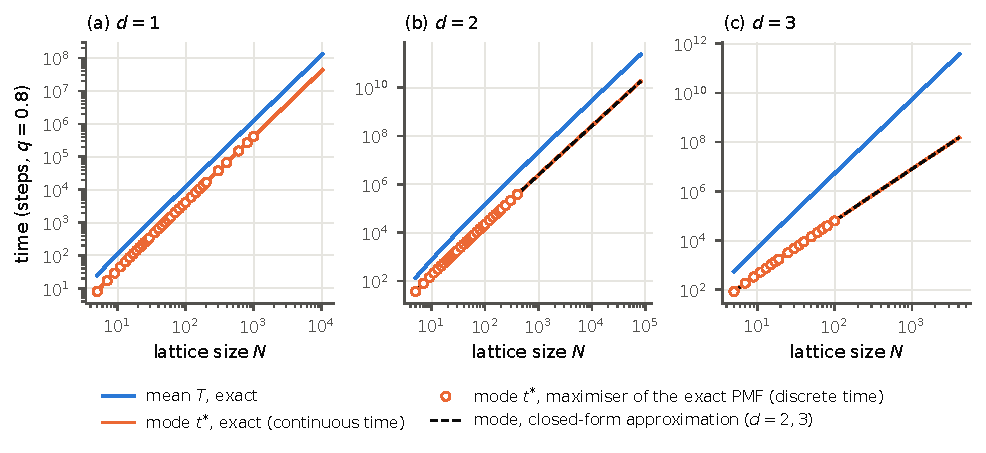
\includegraphics[width=\textwidth]{s5_modes_mode_mean.pdf}
\caption{Mean first-passage time $\MF$ and mode $\tmode$ against lattice size, corner to opposite corner (end to end for
$\dd=1$), in steps at $q=0.8$. Lines: exact values in continuous time (unit rate, divided by $q$). Circles:
maximiser of the exact discrete-time PMF. Dashed: closed-form approximation \eqref{s6_mechanism:eq-L1}.}
% src: code/article/s5_modes_figures.py; data/msc_modes/laplace_modes.jsonl, discrete_modes.jsonl
\label{s5_modes:fig-mode-mean}
\end{figure}

% ---------------------------------------------------------------------------------------------------------
\subsection{One dimension}\label{s5_modes:ssec-1d}

In one dimension the whole distribution is available in closed form (proofs in Supplementary
Section~\ref{sup_modes:ssec-1d-proofs}).

\begin{proposition}[First-passage law of the chain, $\dd=1$]\label{s5_modes:prop-1d}
For the walk on $\{0,\dots,N-1\}$ started at the reflecting end $0$ with target $N-1$, put
$\omega_m=(2m-1)\pi/(2N-1)$ and $\lambda_m=1-q+q\cos\omega_m$, $m=1,\dots,N-1$. Then $\MF=N(N-1)/q$ and, for
all $t\ge1$,
\begin{equation}\label{s5_modes:eq-1d-pmf}
  \pmf(t)=\frac{2q}{2N-1}\sum_{m=1}^{N-1}(-1)^{m+1}\cos\frac{\omega_m}{2}\,\sin\omega_m\;\lambda_m^{\,t-1}.
\end{equation}
\end{proposition}

Put $\ell=N-\tfrac12$, so that $\omega_m=(2m-1)\pi/(2\ell)$ exactly, and let
\begin{equation}\label{s5_modes:eq-1d-continuum}
  \Phi(\xi)=\pi\sum_{m\ge1}(-1)^{m+1}(2m-1)\,
  \exp\Bigl[-\frac{(2m-1)^{2}\pi^{2}}{4}\,\xi\Bigr],\qquad \xi>0 ,
\end{equation}
the first-passage density of diffusion across an interval from a reflecting to an absorbing end, in units of the
diffusion time \citep{Redner2001}; it has mean $\tfrac12$ and variance $\tfrac16$.
% src: data/msc_modes_verify/constants.json; data/article/s5_modes_tables.json (continuum_1d)

\begin{proposition}[Mode-to-mean ratio of the chain]\label{s5_modes:prop-1d-limit}
\begin{enumerate}
\item[(a)] $\Phi$ is log-concave and real-analytic on $(0,\infty)$ and has a unique maximiser $\xi^{*}$, which lies
in $(0.05,0.5)$.
\item[(b)] For the continuous-time walk on the chain, at any activity, $\tmodec/(q\MF)\to2\xi^{*}$ as $N\to\infty$.
\item[(c)] For the discrete-time walk with $q\le\tfrac12$, $\tmode/\MF\to2\xi^{*}$ as $N\to\infty$.
\end{enumerate}
\end{proposition}

The maximiser, computed in 30-digit arithmetic, is $\xi^{*}=0.166642132747$, so that
% src: data/msc_modes_verify/constants.json (1d_tau_star, 1d_mode_over_mfpt); data/msc_modes/fit_results.json (continuum_1d); data/article/s5_modes_tables.json (continuum_1d)
\begin{equation}\label{s5_modes:eq-1d-ratio}
  2\xi^{*}=0.3332842655 ,
\end{equation}
which is the constant $c$ of Theorem~\ref{s6b_rigorous:thm-1d}, enclosed there to within $10^{-70}$. It lies below
$\tfrac13$ by $4.9\times10^{-5}$: the first term of the image expansion of $\Phi$ peaks at exactly $\xi=\tfrac16$, the
mode $(x_0-x_a)^{2}/6$ of direct trajectories discussed by \citet{GodecMetzler2016} (its three-dimensional
counterpart $(r-\rho)^{2}/(6D)$ is Eq.~(3) of \citet{Grebenkov2018}), and the further images move the maximum.
% src: data/msc_rigorous_1d/03_constants.json (c_mid_80_digits, c_radius); data/msc_modes_verify/constants.json (1d_minus_one_third); data/article/s5_modes_tables.json (continuum_1d: one_third_minus_ratio, first_image_term_maximiser)
Proposition~\ref{s5_modes:prop-1d-limit} does not cover the discrete walk at $q=0.8$, where some $\lambda_m$ are
negative; Theorem~\ref{s6b_rigorous:thm-1d} (computer-assisted) does, for every $q\in(0,1]$. At $q=0.8$ the exact modes are
$\tmode=1020$, $4124$, $16\,580$ and $416\,188$ for $N=50$, $100$, $200$ and $1000$, with $\tmode/\MF=0.33306$,
$0.33325$, $0.33327$ and $0.3332837$, and the modes at $N=10^{5}$ and $10^{6}$ give $0.33328427$.
% src: data/msc_modes/tables.md (T1); data/msc_modes/discrete_modes.jsonl; data/article/s5_modes_tables.json (modes_1d_closed_form, modes_1d_large_N, tab_modes_rows); data/msc_modes_verify/bigN_1d_mp.json
The one-dimensional law has a fixed shape: in the continuum limit $\Prob(\FPT\le\tmode)=0.1665$, the median is
$0.7575\,\MF$, the coefficient of variation is $\sqrt{2/3}=0.8165$ and the maximum of the density is $0.925/\MF$.
% src: data/msc_modes_verify/constants.json (1d_cdf_at_mode, 1d_median_over_mfpt, 1d_cv, 1d_gmax_times_mfpt); data/article/s5_modes_tables.json (continuum_1d)

% ---------------------------------------------------------------------------------------------------------
\subsection{Two and three dimensions}\label{s5_modes:ssec-2d}

\begin{observation}[Two dimensions]\label{s5_modes:obs-2d}
The compensated mode $q\tmode/N^{2}$ equals $1.152$, $1.628$, $1.769$, $1.842$ and $1.906$ at $N=5$, $35$, $100$,
$200$ and $401$ and, in continuous time, $2.017$, $2.152$, $2.308$ and $2.390$ at $N=1810$, $20\,480$, $1\,048\,576$
and $16\,777\,216$; it increases, and $\tmode/\MF$ decreases, from each computed size to the next (31 sizes in
discrete time, 43 in continuous time). The ratio $\tmode/\MF$ falls from $0.2696$ at $N=5$ to $0.0562$ at
$N=16\,777\,216$.
% src: data/msc_modes/tables.md (T2); data/msc_modes/summary_tables.md (M2); data/article/s5_modes_tables.json (tab_modes_rows, monotonicity["2"])
\end{observation}

The two-dimensional mode is therefore not proportional to $N^{2}$: its prefactor changes by $60\%$ over
$5\le N\le200$ and keeps growing over the next five decades. The growth is slow: the local exponent
$\dif\ln\tmode/\dif\ln N$ falls from $2.27$ near $N=6$ to $2.06$ near $N=134$ and $2.013$ near $N=3\times10^{6}$, while
that of the mean falls from $2.54$ to $2.20$ and $2.07$.
% src: data/article/s5_modes_tables.json (d2_prefactor_growth_N5_to_200 = 1.599, local_exponents); data/msc_modes/fit_results.json (effective_exponents["2"])
The leading law $q\tmode\simeq(4/\pi^{2})N^{2}[\ln\ln N+\ln8\pi]$ of Section~\ref{s6_mechanism:sec} is a theorem with an
explicit remainder (Theorem~\ref{s6b_rigorous:thm-laws}), but the data do not display it: against $\ln\ln N$ the local
slope of $q\tmode/N^{2}$ decreases from $0.587$ near $N=6$ to $0.451$ near $N=1.2\times10^{7}$, still $11\%$ above
$4/\pi^{2}=0.405$, and the constant $\ln8\pi=3.22$ exceeds $\ln\ln N=2.81$ at the largest size computed; the proved
remainder decays only like $\ln\ln N/\ln N$. We therefore describe the two-dimensional mode by the closed form
\eqref{s6_mechanism:eq-L1-simple}, and use `$N^{2}\ln\ln N$' as the name of its leading asymptote.
% src: data/msc_modes/fit_results.json (asymptotics: 2d_slope_d(mode/N^2)/d(lnlnN), theory_limit); data/article/s5_modes_tables.json (local_slopes, d2_ln_8pi, d2_lnlnN_at_largest_N)

\begin{observation}[Three dimensions]\label{s5_modes:obs-3d}
The compensated mode $q\tmode/N^{2}$ equals $2.72$, $4.43$ and $5.04$ at $N=5$, $40$ and $100$ and, in continuous
time, $5.77$, $6.63$ and $7.34$ at $N=320$, $1280$ and $4096$; it increases, and $\tmode/\MF$ decreases, from each
computed size to the next (17 sizes in discrete time, 27 in continuous time). Against $\ln N$ its local slope is
$0.959$ near $N=6$, $0.636$ near $N=134$ and $0.6095$ near $N=3200$. The ratio $\tmode/\MF$ is $0.1531$, $0.0262$
and $0.0118$ at $N=5$, $40$ and $100$, and $4.1\times10^{-4}$ at $N=4096$.
% src: data/msc_modes/tables.md (T3); data/msc_modes/summary_tables.md (M3); data/msc_modes/fit_results.json (asymptotics: 3d_slope_d(mode/N^2)/d(lnN)); data/article/s5_modes_tables.json (tab_modes_rows, monotonicity["3"], local_slopes)
\end{observation}

Over the computed range the three-dimensional mode thus grows as $N^{2}\ln N$, not as $N^{3}$: the measured slope
$0.6095$ is within $0.3\%$ of the coefficient $6/\pi^{2}=0.6079$ of the proved law (Theorem~\ref{s6b_rigorous:thm-laws}),
the local exponent of the mode falls to $2.085$ near $N=3200$ while that of the mean is $3.0003$, and $\tmode/\MF$ falls
like $\ln N/N$. The three-dimensional maximum is very flat: at $N=40$ the two neighbours of the maximiser lie below the
maximum by relative amounts of only $4\times10^{-10}$ and $2\times10^{-9}$. Its position is resolved by exact
computation (three time-stepping codes and the exact certificates agree), but it is sensitive to small errors in the
PMF (Section~\ref{s6_mechanism:ssec-shape}).
% src: data/msc_modes/fit_results.json (effective_exponents["3"]); data/article/s5_modes_tables.json (local_exponents, stepper_recheck: d = 3, N = 40, "f(mode-1)/f(mode)-1", "f(mode+1)/f(mode)-1"); data/msc_modes_verify/analysis.json (discrete_compare: n_overlap 148, n_mismatch 0); data/article/s3_methods_certificate.json (all_runs.n_mode_equals_stored)

% ---------------------------------------------------------------------------------------------------------
\subsection{The separation between mean and mode grows with dimension}\label{s5_modes:ssec-summary}

Table~\ref{s5_modes:tab-laws} summarises the three cases. At the common size $N=100$ the mean exceeds the mode by the
factors $3.0$, $6.7$ and $85$ for $\dd=1,2,3$; the factor is constant in one dimension, grows logarithmically in two
and almost linearly in three.
% src: data/article/s5_modes_tables.json (separation_T_over_mode)
The reason, made quantitative in Section~\ref{s6_mechanism:sec}, is that the mode is tied to the time of relaxation
across the box, of order $N^{2}$ in every dimension, whereas the mean is tied to the time needed to find the target.
That the most probable first-passage time can lie far below the mean is known for diffusion in confined continuous
domains \citep{GodecMetzler2016,Grebenkov2018}; the lattice values and laws given here are exact counterparts for the
lazy walk.

Scaling fits over short ranges of $N$ cannot reveal these laws. The data are exact, so least-squares intervals
measure misfit, not noise. Fitted on $10\le N\le200$, a free power law $AN^{a}$ gives $a=2.093\pm0.011$ for $\dd=2$,
and the exponent drifts with the window ($2.019\pm0.001$ on $10^{3}\le N\le1.7\times10^{7}$); extrapolated to
$N=16\,777\,216$, the pure quadratic law is off by $-31\%$, the free power law by $+125\%$, the form
$N^{2}(A\ln\ln N+B)$ by $+3.8\%$ and the closed-form approximation \eqref{s6_mechanism:eq-L1}, which has no fitted
parameter, by $-0.45\%$. In three dimensions a cubic law fitted on $10\le N\le100$ over-predicts the mode at $N=4096$ by a
factor $69$, and the closed-form approximation errs by $6\times10^{-7}$ (Supplementary Table~\ref{s5_modes:tab-fits}).
% src: data/msc_modes/tables.md (2D mode fit blocks, row P; extrapolated tables); data/msc_modes/fit_results.json (fits); data/article/s5_modes_tables.json (tab_fits: power_law_exponent_2d_continuous_by_window, N3_fit_overprediction_factor_at_4096 = 68.99)

\begin{table}[tbp]
\centering
\caption{Mean, mode and their ratio, corner to opposite corner. Means: Theorems~\ref{s4_mfpt:thm-cosine} and
\ref{s4_mfpt:thm-expansion} ($\dd=1,2$) and Theorem~\ref{s4_mfpt:thm-3d} ($\dd=3$). Modes: for $\dd=1$ the continuum
constant \eqref{s5_modes:eq-1d-ratio}; for $\dd=2,3$ `$\approx$' marks the closed form \eqref{s6_mechanism:eq-L1-simple}
with $X=\muone q\MF$ (\eqref{s4_mfpt:eq-X2d}, \eqref{s4_mfpt:eq-X3d}), whose scaled error is bounded for every $N\ge12$
($\dd=2$) and $N\ge10$ ($\dd=3$) (Theorem~\ref{s6b_rigorous:thm-cfcont}), and `$\simeq$' the leading laws
(Theorem~\ref{s6b_rigorous:thm-laws}).}
% src: data/article/s4_mfpt_checks.json (three_dimensions: pi2_K3_over_6, pi2_K3prime_over_6); data/msc_modes_verify/constants.json; data/article/closed_form_checks.json (X_const_2d)
\label{s5_modes:tab-laws}
\small
\begin{tabular}{@{}clll@{}}
\toprule
$\dd$ & mean $q\MF$ & mode $q\tmode$ & ratio $\tmode/\MF$\\
\midrule
1 & $N(N-1)$ & $0.33328\,(N-\tfrac12)^{2}$ & $\to0.3332843$\\[5pt]
2 & $\dfrac8\pi N^{2}\ln N+C_{2}N^{2}+\cdots$ &
    $\simeq\dfrac{4}{\pi^{2}}N^{2}\bigl[\ln\ln N+\ln8\pi\bigr]$ &
    $\approx\dfrac{\ln(4X)}{X+3}\simeq\dfrac{\ln(8\pi\ln N)}{2\pi\ln N}$\\[9pt]
3 & $\Kthree N^{3}+\Kthreep N^{2}+\cdots$ &
    $\simeq\dfrac{6}{\pi^{2}}N^{2}\bigl[\ln N+3.753\bigr]$ &
    $\approx\dfrac{\ln(6X)}{X+5}\simeq0.1407\,\dfrac{\ln N+3.753}{N}$\\
\bottomrule
\end{tabular}
\end{table}

% s6_mechanism.tex -- Section 6: pole structure, the closed-form approximation of the mode, and the shape of the law
% (main text; details in Supplementary Section S7).
% Numbers: every quantitative statement carries a comment  % src: <path relative to the root of the repository>.
% Tables are generated by code/article/s6_mechanism_tables.py -> data/article/s6_mechanism_tables.json
% (rows in data/article/s6_mechanism_rows.tex).  Figures: code/article/s3s6_modes_figures.py.
% Vocabulary: "closed-form approximation" is always Eq. (s6_mechanism:eq-L1); the maximiser of the two or three
% slowest exponentials with exact rates and residues is the "exact two-/three-exponential truncation".
\section{Pole structure, a closed-form approximation of the mode, and the shape of the law}\label{s6_mechanism:sec}

This section explains the results of Section~\ref{s5_modes:sec}; Section~\ref{s6b_rigorous:sec} states which parts of
the explanation are proved. We work with the continuous-time walk at unit rate, whose density is
$\gd(t)=\sum_j b_j\eu^{-\nu_j t}$ \eqref{s2_model:eq-spectral} and whose mean is $q\MF$; the discrete-time walk has the same
rates and residues. The propagator of the walk without target in the time domain is
$p(\vx,t\,|\,\vy)=\sum_{\vk}\phi_{\vk}(\vx)\phi_{\vk}(\vy)\eu^{-\mu_{\vk}t}$.

\subsection{Arrival and capture: a factorisation}\label{s6_mechanism:ssec-factor}

\begin{proposition}[Factorisation of the first-passage transform]\label{s6_mechanism:prop-factorisation}
Let $\vo\neq\va$, let $u(t)=\nn\,p(\va,t\,|\,\vo)$ be the occupation of the target site at time $t$ in the walk
without target, normalised by its stationary value $1/\nn$, and let $\FPT_{\mathrm u}$ be the first-passage time to
$\va$ when the start is drawn uniformly from $\Om$ (so that $\FPT_{\mathrm u}=0$ with probability $1/\nn$), with
transform $\Fhat_{\mathrm u}(s)=\E[\eu^{-s\FPT_{\mathrm u}}]$. Then, for $s>0$,
\begin{equation}\label{s6_mechanism:eq-factor}
  \Fhat_{\mathrm u}(s)=\frac{1}{\nn\,s\,\Phat(\va,s\,|\,\va)},\qquad
  \Fhat(s)=\bigl[s\,\hat u(s)\bigr]\,\Fhat_{\mathrm u}(s),
\end{equation}
that is, $\gd(t)=\int_{[0,t]}u'(t-\tau)\,\gd_{\mathrm u}(\dif\tau)$. For the corner start and the opposite corner target,
\begin{equation}\label{s6_mechanism:eq-u}
  u(t)=\Bigl[1+2\sum_{k=1}^{N-1}(-1)^{k}\,\ck{k}^{2}\,\eu^{-\varepsilon_k t}\Bigr]^{\dd},\qquad
  \varepsilon_k=\frac{2}{\dd}\,\sk{k}^{2},
\end{equation}
and for every fixed $x>0$, $u(x/\muone)\to\theta_4(\eu^{-x})^{\dd}$ as $N\to\infty$, where
$\theta_4(y)=1+2\sum_{k\ge1}(-1)^{k}y^{k^{2}}$ is the Jacobi theta function of the nome $y$ \citep[\S20.2]{DLMF}.
\end{proposition}

The proof (Supplementary Section~\ref{sup_mechanism:sec}) averages the renewal ratio over the start. The identity is the
renewal equation written differently, and we do not claim it as new; its use is that it separates the two time scales
of the problem. The factor $u$ describes how the walker \emph{arrives}: it knows nothing about the target and lives on
the diffusive scale $1/\muone\propto N^{2}$. The factor $\Fhat_{\mathrm u}$ describes \emph{capture} from equilibrium,
which for a reversible chain is close to exponential, with an error controlled by the ratio of the relaxation time to
the mean hitting time \citep{AldousBrown1992}, here of order $1/X$. In one dimension $X=2\sk{1}^{2}N(N-1)\to\pi^{2}/2$ is not
large and the two scales coincide; in two and three dimensions $X$ grows as $2\pi\ln N$ and as $7.107\,N$, so the target
is a weak sink on the diffusive scale.
% src: data/article/s6_mechanism_tables.json (asymptotes: X_const_2d = 0.38155, pi2_K3_over_6 = 7.10687)

\subsection{Formal two-pole asymptotics}\label{s6_mechanism:ssec-two-pole}

\begin{heuristic}[Closed-form approximation of the mode]\label{s6_mechanism:res-L1}
Let $\mu$ be the smallest non-zero relaxation rate (unit rate) of the reflecting lattice whose eigenspace has
non-zero weight at the target, $W=\nn\sum_{\mu_{\vk}=\mu}\phi_{\vk}(\va)^{2}$ that weight and
$A=-\nn\sum_{\mu_{\vk}=\mu}\phi_{\vk}(\va)\phi_{\vk}(\vo)$ the corresponding amplitude seen from the start, and let
$X=\mu\,q\MF$. If $A>0$ and $X\gg1$, the mode of the continuous-time first-passage density at unit rate is
\begin{equation}\label{s6_mechanism:eq-L1}
  \tmodec\;\approx\;q\MF\;\frac{\ln(A X)}{X+W-1},
\end{equation}
and the discrete-time mode at activity $q$ is $\tmode\approx\tmodec/q$. For corner-to-corner transport
$\mu=\muone=\tfrac{2}{\dd}\sin^{2}\tfrac{\pi}{2N}$ and $A=W=2\dd\cos^{2}\tfrac{\pi}{2N}$; replacing $\cos^{2}$ by 1 gives the
simplified form
\begin{equation}\label{s6_mechanism:eq-L1-simple}
  \frac{\tmode}{\MF}\;\approx\;\frac{\ln(2\dd X)}{X+2\dd-1},\qquad X=\muone\,q\MF .
\end{equation}
\end{heuristic}

\noindent We write $\tcf:=\MF\ln(2\dd X)/(X+2\dd-1)$ for the approximation of the discrete-time mode given by
\eqref{s6_mechanism:eq-L1-simple}; in Section~\ref{s6b_rigorous:sec} and in the accuracy statements of the Introduction
and of Section~\ref{s9_discussion:sec}, ``the closed form'' means $\tcf$, whereas ``the closed-form approximation''
\eqref{s6_mechanism:eq-L1} keeps the factors $A$ and $W$.

\noindent\emph{Derivation.} Separate the uniform eigenvector (rate $0$) and the eigenspace of $\mu$:
\begin{equation}\label{s6_mechanism:eq-split}
  \nn\,\Phat(\va,s\,|\,\va)=\frac1s+\frac{W}{s+\mu}+R(s),\qquad
  \hat u(s)=\nn\,\Phat(\va,s\,|\,\vo)=\frac1s-\frac{A}{s+\mu}+R_{\vo}(s),
\end{equation}
where $R$ and $R_{\vo}$ collect the eigenvalues $\mu_{\vk}>\mu$ and are analytic for $\operatorname{Re}s>-\mu'$, $\mu'$
being the next rate with weight at the target. The poles of $\Fhat$ are the zeros $-\nu_j$ of the first function, with
$0<\nu_0<\mu<\nu_1<\mu'$ (Proposition~\ref{s2_model:prop-interlacing}), and
$b_j=\hat u(-\nu_j)\big/\nn\,\partial_s\Phat(\va,s\,|\,\va)\big|_{s=-\nu_j}$. The limit $s\to0$ of $(1-\Fhat)/s$ gives
$q\MF=(W+A)/\mu+R(0)-R_{\vo}(0)$. \emph{Assume} that $X\gg1$, that $R$ varies by a relative amount $\Order(1/X)$ on
$[-\nu_1,0]$ with $R(0)=q\MF\,(1+\Order(1/X))$, and that $R_{\vo}=\Order(1/\mu)$ there. The two zero conditions then give
\begin{equation}\label{s6_mechanism:eq-poles}
  \nu_0=\frac{1}{q\MF}\bigl(1+\Order(X^{-1})\bigr),\qquad
  \nu_1=\mu\Bigl(1+\frac{W}{X}+\Order(X^{-2})\Bigr),\qquad
  b_0\approx\nu_0,\qquad b_1\approx-A\,\nu_0 .
\end{equation}
Keeping only $j=0,1$ in $\gd'(t)=-\sum_j b_j\nu_j\eu^{-\nu_j t}$ and solving $\gd'=0$ (possible because $b_1<0$, that is,
$A>0$) gives $\tmodec=\ln(-b_1\nu_1/b_0\nu_0)/(\nu_1-\nu_0)$. To leading order,
\begin{equation}\label{s6_mechanism:eq-L0}
  \tmodec\;\approx\;\frac{\ln(AX)}{\mu},
\end{equation}
and inserting the first-order rate difference $\nu_1-\nu_0=\mu\,(X+W-1)/X$ while keeping the argument of the logarithm at
its leading value $AX$ gives \eqref{s6_mechanism:eq-L1}.

\medskip\noindent\emph{Status.} This is a derivation, not a proof: it needs (i) uniform bounds on $R$ and $R'$, (ii) a bound
on the poles $j\ge2$, and (iii) unimodality. For corner-to-corner transport in two and three dimensions
Section~\ref{s6b_rigorous:sec} supplies all three by a route that does not expand $R$, and proves that
$X\muone(\tmodec-q\tcf)$ stays in a bounded window, a relative error $\Order(1/(X\ln X))$ for \eqref{s6_mechanism:eq-L1-simple}
(Theorem~\ref{s6b_rigorous:thm-cfcont}); the relations \eqref{s6_mechanism:eq-poles} are
Theorem~\ref{s6b_rigorous:thm-poles}(c). In one dimension the assumption $X\gg1$ fails and so does the formula (Refuted
statement~\ref{s6b_rigorous:ref-cf1d}). Equation~\eqref{s6_mechanism:eq-L1} is not a consistent expansion to order
$1/X$; the omitted terms partly cancel (Supplementary Section~\ref{sup_mechanism:ssec-ingredients}).

\subsection{Accuracy and leading laws}\label{s6_mechanism:ssec-accuracy}

Table~\ref{s6_mechanism:tab-accuracy} compares the predictions with the exact continuous-time modes, on the computed
grid of 41 sizes with $10\le N\le16\,777\,216$ for $\dd=2$ and 25 sizes with $10\le N\le4096$ for $\dd=3$.
% src: data/article/s6_mechanism_tables.json (accuracy/2d_CC, 3d_CC: n_sizes_N>=10); data/article/closed_form_checks.json
The leading-order form \eqref{s6_mechanism:eq-L0} errs by $+19.9\%$ at $N=10$ and still by $+2.4\%$ at $N=16\,777\,216$
for $\dd=2$. The closed-form approximation \eqref{s6_mechanism:eq-L1} is within $0.972\%$ of the exact mode for $\dd=2$
(worst at $N=113$) and within $0.289\%$ for $\dd=3$ (worst at $N=10$; within $1.3\times10^{-5}$ for $N\ge100$); the simplified
form \eqref{s6_mechanism:eq-L1-simple} is within $0.970\%$ and $0.085\%$. In two dimensions the error decreases slowly, to
$-0.45\%$ at $N=16\,777\,216$, where $X$ is only $104.9$. The errors of \eqref{s6_mechanism:eq-L1-simple} at the 40 sizes
with $N\ge12$ ($\dd=2$) and at all 25 sizes ($\dd=3$) lie inside the windows of Theorem~\ref{s6b_rigorous:thm-cfcont};
for $\dd=2$, $N=10$ no window is proved. With the two-term mean of Theorem~\ref{s4_mfpt:thm-expansion} and $X$ from
\eqref{s4_mfpt:eq-X2d}, so that no exact input is needed, the error of \eqref{s6_mechanism:eq-L1-simple} stays within
$0.975\%$ for $\dd=2$. The exact three-exponential truncation is within $5.35\times10^{-5}$ ($\dd=2$) and $7.1\times10^{-6}$
($\dd=3$): the mode is controlled by very few poles.
% src: data/article/closed_form_checks.json (2d_CC, 3d_CC: L1_weights, L1_plain, L0; 2d_CC_fully_asymptotic_L1_plain); data/article/s6_mechanism_tables.json (accuracy; accuracy/2d_CC/rows; three_pole); data/msc_modes/summary_tables.md (M2); data/article/s6b_rigorous_checks.json (continuous_time_against_windows: n_sizes_in_window_range, n_inside_window)

\begin{table}[tbp]
\centering
\caption{Signed relative error (in per cent, except the last column) of five predictions of the exact
continuous-time mode, corner to corner, unit rate: the leading-order form \eqref{s6_mechanism:eq-L0}; the
closed-form approximation \eqref{s6_mechanism:eq-L1} with $A=W=2\dd\cos^{2}(\pi/2N)$; its simplified form
\eqref{s6_mechanism:eq-L1-simple}; and the exact two- and three-exponential truncations, that is, the maximiser of
the two or three slowest exponentials with numerically exact rates and residues (last column: relative error, not
per cent). No parameter is fitted.}
\label{s6_mechanism:tab-accuracy}
% src: data/article/s6_mechanism_rows.tex, s6_mechanism_tables.json (accuracy/*/rows), computed by code/article/s6_mechanism_tables.py from data/msc_modes/laplace_modes.jsonl; L1 and L1s columns agree with data/article/closed_form_checks.json; L0, L1, two- and three-pole columns agree with data/msc_modes/summary_tables.md (M2, M3)
\small
\begin{tabular}{rrrrrrr}
\toprule
$N$ & $X$ & \eqref{s6_mechanism:eq-L0} (\%) & \eqref{s6_mechanism:eq-L1} (\%) & \eqref{s6_mechanism:eq-L1-simple} (\%) & two exp.\ (\%) & three exp.\\
\midrule
\multicolumn{7}{l}{$\dd=2$}\\
10 & 14.740 & $+19.939$ & $+0.2096$ & $+0.2660$ & $+0.6602$ & $+5.3\times10^{-5}$ \\
35 & 22.706 & $+12.231$ & $-0.8354$ & $-0.8222$ & $+0.5134$ & $+5.5\times10^{-6}$ \\
113 & 30.083 & $+8.901$ & $-0.9717$ & $-0.9700$ & $+0.3904$ & $+1.6\times10^{-6}$ \\
1280 & 45.335 & $+5.695$ & $-0.8654$ & $-0.8654$ & $+0.2437$ & $+3.1\times10^{-7}$ \\
10\,240 & 58.401 & $+4.361$ & $-0.7384$ & $-0.7384$ & $+0.1791$ & $+1.2\times10^{-7}$ \\
1\,048\,576 & 87.485 & $+2.876$ & $-0.5347$ & $-0.5347$ & $+0.1089$ & $+2.6\times10^{-8}$ \\
16\,777\,216 & 104.906 & $+2.392$ & $-0.4545$ & $-0.4545$ & $+0.0871$ & $+1.4\times10^{-8}$ \\
\midrule
\multicolumn{7}{l}{$\dd=3$}\\
10 & 64.168 & $+7.253$ & $-0.2886$ & $-0.0845$ & $+0.1544$ & $-7.1\times10^{-6}$ \\
35 & 242.186 & $+2.034$ & $-0.0253$ & $-0.0025$ & $+0.0365$ & $-3.1\times10^{-7}$ \\
100 & 704.235 & $+0.708$ & $-0.0013$ & $+0.0015$ & $+0.0112$ & $-2.9\times10^{-8}$ \\
320 & 2267.787 & $+0.221$ & $+0.0005$ & $+0.0008$ & $+0.0031$ & $-2.3\times10^{-9}$ \\
1280 & 9090.397 & $+0.055$ & $+0.0002$ & $+0.0002$ & $+0.0007$ & $-1.3\times10^{-10}$ \\
4096 & 29\,103.352 & $+0.017$ & $+0.0001$ & $+0.0001$ & $+0.0002$ & $+9.6\times10^{-11}$ \\
\bottomrule
\end{tabular}
\end{table}

With $1/\muone\simeq2\dd N^{2}/\pi^{2}$, $X\simeq2\pi\ln N$ for $\dd=2$ and $X\simeq\pi^{2}\Kthree N/6$ for $\dd=3$, the
leading-order form \eqref{s6_mechanism:eq-L0} becomes
\begin{equation}\label{s6_mechanism:eq-asym-2d}
  \dd=2:\qquad q\,\tmode\simeq\frac{4}{\pi^{2}}\,N^{2}\bigl[\ln\ln N+\ln 8\pi\bigr],\qquad
  \frac{\tmode}{\MF}\simeq\frac{\ln(8\pi\ln N)}{2\pi\ln N},
\end{equation}
\begin{equation}\label{s6_mechanism:eq-asym-3d}
  \dd=3:\qquad
  \begin{aligned}
  q\,\tmode&\simeq\frac{6}{\pi^{2}}\,N^{2}\bigl[\ln N+\ln(\pi^{2}\Kthree)\bigr]=0.6079\,N^{2}\,(\ln N+3.7528),\\
  \frac{\tmode}{\MF}&\simeq0.1407\,\frac{\ln N+3.753}{N}.
  \end{aligned}
\end{equation}
% src: data/article/s6_mechanism_tables.json (asymptotes: 6_over_pi2 = 0.60793, ln_pi2_K3 = 3.75282, 6/(pi^2 K3) = 0.14071)
Both laws are theorems with explicit remainders (Theorems~\ref{s6b_rigorous:thm-laws} and~\ref{s6b_rigorous:thm-disc}). In
three dimensions the law is visible in the data: it exceeds the exact $\tmodec/N^{2}$ by $8.7\%$ at $N=10$, $0.81\%$ at
$N=100$ and $0.02\%$ at $N=4096$. In two dimensions it is not: the constant $\ln8\pi=3.22$ exceeds $\ln\ln N$ for every
$N<\eu^{8\pi}\approx8\times10^{10}$, and the law exceeds the exact value by $19\%$, $8.9\%$ and $2.3\%$ at $N=10$, $100$ and
$16\,777\,216$. At every accessible size the two-dimensional mode should be described by
\eqref{s6_mechanism:eq-L1-simple}, not by its leading term.
% src: data/article/s6_mechanism_tables.json (asymptotes/3d: rel_err; asymptotes: ln_8pi, exp_8pi, 2d rel_err)

\subsection{Shape of the law: the mode is not a typical time}\label{s6_mechanism:ssec-shape}

Proposition~\ref{s6_mechanism:prop-factorisation} also describes the whole density. If $\gd_{\mathrm u}$ is replaced by the
exponential law of rate $\nu_0$, then $\gd(t)\approx\nu_0\int_0^{t}u'(\tau)\eu^{-\nu_0(t-\tau)}\dif\tau$, which is $\nu_0u(t)$ for
$t\ll q\MF$ and $\nu_0\eu^{-\nu_0t}$ for $t\gg1/\muone$, and whose maximum is where the late-time arrival rate
$u'(t)\approx A\mu\eu^{-\mu t}$ has dropped to the capture rate $\nu_0$, which is \eqref{s6_mechanism:eq-L0}.
Figure~\ref{s6_mechanism:fig-density} shows both regimes for the exact densities: in the variable $x=\muone t$ the product
$q\MF\,\gd$ follows $\theta_4(\eu^{-x})^{\dd}$ up to the maximum, and in the variable $t/(q\MF)$ it follows $\eu^{-t/(q\MF)}$.
There is no single-scale collapse.

\begin{figure}[tbp]
\centering
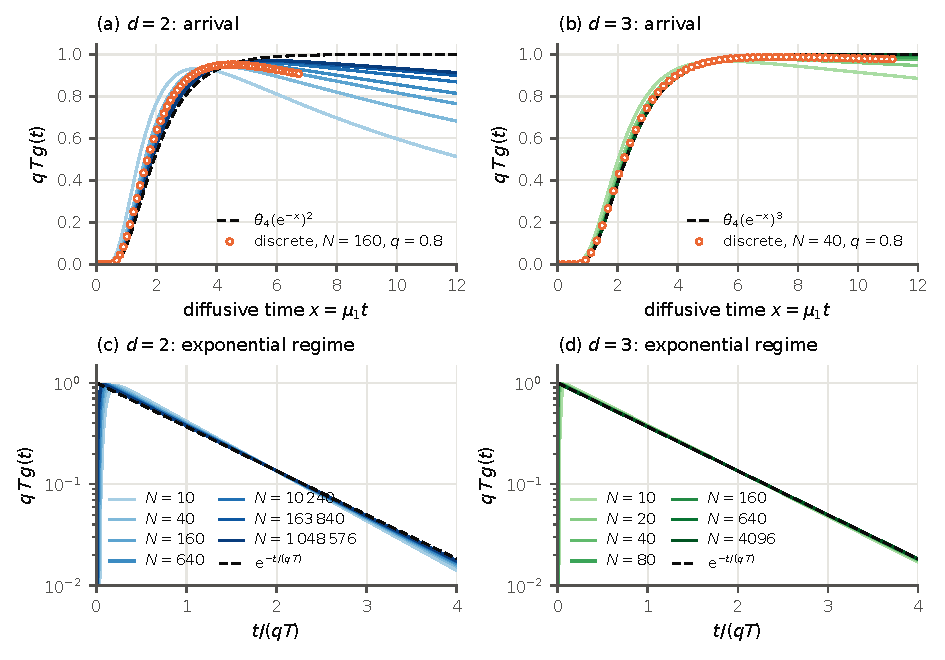
\includegraphics[width=\textwidth]{s6_mechanism_density.pdf}
\caption{Exact first-passage densities, corner to corner, continuous time at unit rate (lines; sizes and colours
as listed in panels (c) and (d)). (a,b) Against the diffusive time $x=\muone t$, for $\dd=2$ ($N=10$ to
$1\,048\,576$) and $\dd=3$ ($N=10$ to $4096$); dashed: $\theta_4(\eu^{-x})^{\dd}$; open circles: exact discrete-time
$\MF\,\pmf(t)$ at $q=0.8$ for $N=160$ ($\dd=2$) and $N=40$ ($\dd=3$), plotted against $\muone qt$. (c,d) The same
densities against $t/(q\MF)$ on a logarithmic scale; dashed: $\eu^{-t/(q\MF)}$.}
\label{s6_mechanism:fig-density}
% src: code/article/s3s6_modes_figures.py; data data/msc_modes/profiles.npz, data/msc_modes/profile_stats.json, data/msc_modes/pmf/
\end{figure}

\begin{table}[tbp]
\centering
\caption{Shape statistics of the exact first-passage law, corner to corner, continuous time at unit rate:
mode-to-mean ratio, probability of arrival by the modal time, median, survival at the mean, height of the
density at the mode in units of $1/q\MF$ (equal to 1 for an exponential law), and the window, in units of
$\tmodec$, in which the density exceeds $99\%$ of its maximum. For $\dd=1$ the start is the reflecting end.}
\label{s6_mechanism:tab-shape}
% src: data/article/s6_mechanism_rows.tex, s6_mechanism_tables.json (shape_table): columns 3-6 from data/msc_modes/medians.json; columns 7-8 recomputed by code/article/s6_mechanism_tables.py with code/msc_modes/fptlib.py (agree with data/msc_modes/profile_stats.json at the two sizes in common, differences below 4e-11)
\small
\begin{tabular}{rrcccccc}
\toprule
$\dd$ & $N$ & $\tmodec/q\MF$ & $\Prob(\FPT\le\tmodec)$ & median$/q\MF$ & $\Sv(q\MF)$ & $\gd(\tmodec)\,q\MF$ & $99\%$ window\\
\midrule
1 & 1000 & 0.3333 & 0.1665 & 0.7575 & 0.3708 & 0.9251 & $[0.89,\,1.13]$ \\
2 & 35 & 0.1769 & 0.0981 & 0.7195 & 0.3683 & 0.9448 & $[0.87,\,1.17]$ \\
2 & 200 & 0.1350 & 0.0780 & 0.7117 & 0.3681 & 0.9529 & $[0.85,\,1.19]$ \\
2 & 163\,840 & 0.0729 & 0.0456 & 0.7017 & 0.3679 & 0.9690 & $[0.82,\,1.27]$ \\
3 & 40 & 0.0262 & 0.0174 & 0.6959 & 0.3679 & 0.9879 & $[0.77,\,1.51]$ \\
3 & 100 & 0.0118 & 0.0082 & 0.6942 & 0.3679 & 0.9939 & $[0.72,\,1.97]$ \\
3 & 1280 & 0.0012 & 0.0009 & 0.6932 & 0.3679 & 0.9992 & $[0.58,\,9.47]$ \\
\bottomrule
\end{tabular}
\end{table}

Table~\ref{s6_mechanism:tab-shape} quantifies the consequence. For $\dd\ge2$ the first-passage law to a distant point
target is an exponential law preceded by a short dead time, not a peaked law with a long tail. Only $9.8\%$ ($\dd=2$,
$N=35$) and $1.7\%$ ($\dd=3$, $N=40$) of the walkers have arrived by the modal time, and this fraction decreases with $N$;
the median is $0.72\,\MF$ and $0.70\,\MF$ and approaches $\ln2=0.693$; the survival probability at the mean is $0.3683$ and
$0.3679$ against $1/\eu=0.3679$. The tail is exponential (geometric in discrete time) with rate $\nu_0$, not algebraic.
% src: data/msc_modes/medians.json; data/msc_modes/summary_tables.md (S, Md); data/article/s6_mechanism_tables.json (shape_table)
The maximum is also flat, increasingly so with dimension and size: for $\dd=3$ the density stays within $1\%$ of its
maximum from $0.58$ to $9.5$ modal times at $N=1280$, and at $\dd=3$, $N=100$ a relative error of $1\%$ in the density can
displace the apparent maximum anywhere between $0.72$ and $1.97$ modal times. The mode is therefore a soft statistic: it
marks the end of the dead time, it is not a typical arrival time, and the median is the appropriate typical value.
Statements about waiting times must be made with $\Sv$: the fraction of searches still unfinished is $36.8\%$ at
$t=\MF$, and $90\%$ ($\dd=2$, $N=35$) or $98\%$ ($\dd=3$, $N=40$) at $t=\tmode$.
% src: data/article/s6_mechanism_tables.json (shape_table, N = 1280); data/msc_modes/medians.json (S_at_mfpt 0.36827, 0.36788; S_at_mode 0.90189, 0.98261)

None of this structure is new in kind. Two time scales in confinement, and an exponential law rescaled by the mean
when the target is hard to find, are established for continuous and scale-invariant processes
\citep{Benichou2010,GodecMetzler2016}, and the rescaled laws fall into universality classes \citep{Meyer2011}; that the
mean may then be unrepresentative, and the most probable time far below it, is the subject of \citet{Mattos2012},
\citet{GodecMetzler2016} and \citet{Grebenkov2018}; and the exponential approximation for reversible chains is classical
\citep{AldousBrown1992}. In particular, \citet[Eq.~(31)]{Grebenkov2018} note that the median is close to $\ln2$ times the
mean when the survival probability is nearly exponential, which explains the limit $\ln2$ above, and give the
most probable time of the direct trajectories, $(r-\rho)^{2}/(6D)$ for a spherical target of radius $\rho$ at distance
$r$ \citep[Eq.~(3)]{Grebenkov2018}, the continuum counterpart of the first-image term of Section~\ref{s5_modes:sec}.
That estimate does not locate the mode of corner-to-corner transport for $\dd\ge2$: there the mode is set by the
relaxation of the box, $\tmode\approx\ln(AX)/(q\mu)$ for large $X$ by \eqref{s6_mechanism:eq-L1}, a time of order
$N^{2}\ln(AX)$ whose logarithmic factor grows with $N$, whereas the direct-trajectory time is of order $N^{2}$ with no
such factor. The relations
\eqref{s6_mechanism:eq-poles} are the lattice analogue of the perturbation of eigenvalues by a small removed region
\citep{WardKeller1993}, and uniform approximations of the density to a small target were given by
\citet{IsaacsonNewby2013}, who obtain the mode by maximising the density numerically, without a closed formula.
% src: Isaacson and Newby (2013), full text consulted in arXiv:1303.3016 (Eqs (2.11), (2.47)-(2.49); Sec. III.1; caption of Fig. 7: "we compute the mode by numerically maximizing the first passage time density")
% provenance of the attributions above: full texts read of IsaacsonNewby2013 (arXiv:1303.3016), GodecMetzler2016
% (arXiv:1611.07788), Benichou2010 (arXiv:1006.3477, rescaled FPT law exponential for non-compact exploration),
% Mattos2012 (arXiv:1206.1003) and Grebenkov2018 (arXiv:1911.00942, Eqs (3), (31)); Meyer2011 and WardKeller1993 are
% cited only for what their abstracts state (see the citedfor fields of refs.bib)
What is added here is the exact computation for the lattice walk, the dimension dependence of its mode, and the explicit
closed-form approximation \eqref{s6_mechanism:eq-L1} and closed form \eqref{s6_mechanism:eq-L1-simple} with their
measured accuracy; we do not know whether these formulas appear elsewhere and make no claim of priority.

\subsection{Other placements and the activity}\label{s6_mechanism:ssec-geometries}

For a corner start and a centre target (\CtM, odd $N$) the modes with $k_i=1$ vanish at the target, so that
$\mu=\tfrac{2}{\dd}\sin^{2}\tfrac{\pi}{N}\approx4\muone$, $W=2\dd$ and $A=2\dd\cos\tfrac{\pi}{N}$, and
\eqref{s6_mechanism:eq-L1} is within $0.964\%$ ($\dd=2$, 24 sizes, $11\le N\le655\,361$) and $0.206\%$ ($\dd=3$, 15
sizes, $11\le N\le1281$) of the exact mode. For a centre start and a corner target (\MtC) the formula does not apply:
the slowest mode seen by the target vanishes at the start ($A=0$), the residue $b_1$ is positive, and the maximum is set
by the first arrivals, to which several poles contribute; the mode is nevertheless far below the mean, with exact
discrete ratios $0.0352$ ($\dd=2$, $N=201$) and $0.0046$ ($\dd=3$, $N=61$) at $q=0.8$. For exit from the centre through an
absorbing boundary layer there is no small parameter, and $\tmode/\MF$ tends to a constant, $0.333284$, $0.474907$ and
$0.560839$ for $\dd=1,2,3$. Details are in Supplementary Section~\ref{sup_mechanism:ssec-geometries}.
% src: data/article/closed_form_checks.json (2d_C2M, 3d_C2M); data/article/s6_mechanism_tables.json (accuracy/2d_C2M, 3d_C2M; c2m_weights_check); data/msc_modes/discrete_modes.jsonl (M2C, q = 0.8: N = 201 ratio 0.035209; N = 61 ratio 0.004590); data/msc_modes/fit_results.json (continuum_exit)

By Proposition~\ref{s2_model:prop-structure}, $q\MF$ and $q$ times the continuous-time mode do not depend on $q$, and the
discrete-time mode inherits this up to a few steps: for $\dd=2$, $N=101$ the exact argmax times $q$ is $18\,056.1$,
$18\,056.0$, $18\,055.8$ and $18\,056$ for $q=0.3$, $0.5$, $0.9$ and $1$, against $\tmodec=18\,056.39$. Hence
$\tmode/\MF$ does not depend on $q$ beyond terms of order $1/\MF$.
% src: data/msc_modes/summary_tables.md (Q); data/msc_modes/discrete_modes.jsonl (group qscan); data/article/s6_mechanism_tables.json (activity)

% s6b_rigorous.tex -- Section 7: what is proved about the first-passage law and its mode (main text).
% Sources: the companion notes R0-R5 (folder proofs/ of the repository).  Every number carries a comment
%   % src: <path relative to the root of the repository>.  Consistency checks against the computations of Sections 3-6:
%   code/article/s6b_rigorous_checks.py -> data/article/s6b_rigorous_checks.json.
% Proofs: Supplementary Section S8 (appD_rigorous.tex) and the companion notes.
\section{What is proved about the first-passage law and its mode}\label{s6b_rigorous:sec}

Sections~\ref{s5_modes:sec} and~\ref{s6_mechanism:sec} rest on exact computation at the sizes run and on the formal
argument of Section~\ref{s6_mechanism:ssec-two-pole}. This section states what is proved. Short proofs are in
Supplementary Section~\ref{appD_rigorous:sec}; long proofs and the computer-assisted ones are in the companion notes.

\subsection{Status of the statements, sources and checks}\label{s6b_rigorous:ssec-status}

\paragraph{Companion notes.} The complete proofs are contained in six notes (R0--R5, 32 to 51 pages each) in the
folder \texttt{proofs/} of the repository \citep{ZhouyiRepo}, cited as \Sref{R0}{\dots}, \dots, \Sref{R5}{\dots} with their own statement numbers:
R0, a dependency-ordered account of all results with a table of their status, the certificates and their trusted bases
\citep{NoteR0}; R1, the walk on the segment \citep{NoteR1}; R2, the spectral structure of the first-passage law
\citep{NoteR2}; R3, the mode of the corner-to-corner law in two and three dimensions \citep{NoteR3}; R4, unimodality
\citep{NoteR4}; R5, exact certified computations \citep{NoteR5}. The notes number sites from $1$ to
$N$; their $\Lambda_1$, $\sigma_j$, $r_j$, $m(\vo)$, $\tau$, $C_3$, $C_3'$ are our $\muone$, $\nu_j$, $b_j/\nu_j$, $q\MF$,
$\tau_{\mathrm u}$, $\Kthree$, $\Kthreep$.
% src: proofs/R0_rigorous_results/R0_rigorous_results.tex (Sections 2, 3: notation, dictionary and summary table)

\paragraph{Status words.} \emph{Theorem}, \emph{Proposition}, \emph{Lemma} and \emph{Corollary} mean a complete proof.
\emph{Theorem (computer-assisted)} means that the proof reduces the statement, by lemmas proved by hand, to finitely many
inequalities that a program verifies in exact integer or rational arithmetic or in rigorous ball arithmetic. Three
trusted bases occur (labelled as in \Sref{R0}{Section 9}; the bases T2 and T4 defined there do not enter the statements
of this article): (T1) Python integers and fractions; (T3) ball arithmetic of the Arb library, through
python-flint~0.9.0, together with the transcription of the formulas into the certification scripts; (T5) a C program of
366 lines with unsigned 64- and 128-bit integer arithmetic whose output is turned into verdicts with Python integers.
For 2242 of the 3824 certificates of the C program, all beyond the ranges covered with Python integers, that program,
run twice with identical checksums, is the only witness.
Every statement names its base; the certificates and the programs that check them are in the repository. No program
has been verified in a proof assistant, and floating-point arithmetic is used only to find candidates, never to decide.
\emph{Formal result} means a derivation by formal asymptotics, \emph{Numerical observation} a statement established by
exact computation at the sizes stated only, and \emph{Refuted statement} a natural conjecture, suggested by the
one-dimensional case or by numerical evidence, that is false.
% src: proofs/R0_rigorous_results/R0_rigorous_results.tex (Section 9: trusted bases T1-T5; certificate table; separately written re-checks: 2242 of 3824)

\paragraph{Verification and reproducibility.} The proof notes supply the analytical reductions and identify the arithmetic certificates supporting each computer-assisted statement. The scripts in the repository check the one-dimensional constants, the spectral bounds, the Taylor-model inequalities for unimodality, and the finite-range mode certificates. The discrete-time window for every $q<1$ is verified under its stated size condition by regenerating the ball-arithmetic certificate and checking the complete block coverage. The commands and their coverage are documented in \texttt{submission/SCIENTIFIC-CHECKS.md}; the detailed derivations remain in the companion notes. The trusted bases and the parameter restrictions stated above are unchanged.

% ---------------------------------------------------------------------------------------------------------
\subsection{The first-passage law: structure and signs}\label{s6b_rigorous:ssec-structure}

Here the rates are indexed by all zeros of Proposition~\ref{s2_model:prop-interlacing}(i), $\nu_j:=\nu_{(j)}$, with
$b_j=0$ when the pole is absent from the law started at $\vo$. We write $r_j:=b_j/\nu_j$ for the weights of the survival
function, $\Sv(t)=\sum_jr_j(1-q\nu_j)^{t}$, so that $\sum_jr_j=1$, and $D=|\vo-\va|_1$ for the graph distance.

\begin{theorem}[Signs of the residues]\label{s6b_rigorous:thm-signs}
For every symmetric chain of Section~\ref{s2_model:sec} (any $N$, $\dd$, start and target):
\begin{enumerate}
\item[(a)] $\sum_jr_j\nu_j^{\,i}=0$ for $1\le i\le D-1$ and $(-1)^{D-1}\sum_jr_j\nu_j^{\,D}>0$; hence the sequence
$(r_j)$ has at least $D-1$ changes of sign. For the chain started at its reflecting end, the number of rates is
$D=N-1$ and the signs alternate, $\operatorname{sign}r_j=(-1)^j$.
\item[(b)] From the uniform start the law is, apart from the atom $1/\nn$ at $t=0$, a mixture of exponential laws
with positive weights (of geometric laws in discrete time, for $q\le\frac12$).
\item[(c)] From the quasi-stationary distribution the first-passage time is exactly exponential with rate $\nu_0$
(geometric in discrete time).
\end{enumerate}
\textup{(Source: \Sref{R2}{Thm 5.1, Props 5.4, 5.5}, \Sref{R4}{Thm 3.2}; (b) and (c) are classical for reversible
chains \citep{AldousFill}.)}
\end{theorem}

\begin{theorem}[A single distant start is never a mixture]\label{s6b_rigorous:thm-notmixture}
If $D\ge2$, there is no positive measure $m$ on $[0,\infty)$ with $\gd(t)=\int\eu^{-\sigma t}m(\dif\sigma)$ for all
$t>0$, and none on $[0,1)$ with $\pmf(t)=\int\lambda^{t-1}m(\dif\lambda)$ for all $t\ge1$; in particular some residue
$b_j$ is negative.
\textup{(Source: \Sref{R4}{Thm 4.1(d)}.)}
\end{theorem}

\begin{theorem}[Signs of the corner-to-corner residues]\label{s6b_rigorous:thm-alternation}
For the corner-to-corner pair:
(a) if $\dd\ge2$, then $r_0>0>r_1$ for every $N\ge2$;
(b) if $\dd=1$ or $N=2$, the number of rates is $D=\dd(N-1)$ and $\operatorname{sign}r_j=(-1)^j$;
(c) if $\dd\ge2$ and $N\ge3$, the residues do not alternate in sign: there are three consecutive residues
whose signs form a monotone sequence.
\textup{(Source: \Sref{R2}{Cor 5.7, Prop 5.9, Thm 5.10}.)}
\end{theorem}

\begin{refuted}\label{s6b_rigorous:ref-alternation}
``The residues of the corner-to-corner law alternate in sign in every dimension, as they do in one dimension.''
False for every $\dd\ge2$ and $N\ge3$ by Theorem~\ref{s6b_rigorous:thm-alternation}(c). The smallest example is
$\dd=2$, $N=3$, where the five residues have the signs $+,-,-,+,-$ (certified in ball arithmetic).
\textup{(Source: \Sref{R2}{Section 5.2, Prop 14.1}.)}
% src: data/msc_rigorous_spectral/13_certified_residue_signs.json
\end{refuted}

Descartes' rule bounds the number of zeros of $\gd'$ by the number of sign changes of the residues, which is at least
$D-1$; for $\dd\ge2$ and $N\ge3$ it cannot prove unimodality, and the proofs below use log-concavity instead. Let
$\tau_{\mathrm u}=q\,\E\FPT_{\mathrm u}$ be the unit-rate mean first-passage time from the uniform start
(Proposition~\ref{s6_mechanism:prop-factorisation}) and $\bar X=\muone\tau_{\mathrm u}$.

\begin{theorem}[The two slowest poles]\label{s6b_rigorous:thm-poles}
\begin{enumerate}
\item[(a)] For every target, $\tau_{\mathrm u}\le1/\nu_0\le\tau_{\mathrm u}+1/\mu_{(1)}$.
\item[(b)] For the corner-to-corner pair, every $\dd\ge1$ and $N\ge2$ with $(\dd,N)\ne(1,2)$: $r_0>1$ and
$\nu_0\,q\MF>1$.
\item[(c)] For the corner-to-corner pair in $\dd=2,3$, as $N\to\infty$,
\begin{gather*}
\nu_0\,q\MF=1+\frac{\mu_\infty}{\bar X}+o(\bar X^{-1}),\qquad
r_0=1+\frac{\mu_\infty}{\bar X}+o(\bar X^{-1}),\\
\frac{\nu_1-\nu_0}{\muone}=1+\frac{2\dd-1}{\bar X}+\Order(\bar X^{-2}),\qquad \frac{b_1}{b_0}\to-2\dd ,
\end{gather*}
where $\mu_\infty:=\lim_{N\to\infty}(X-\bar X)$, a limit that exists, with $\mu_\infty=\pi\ln2$ for $\dd=2$ and
$\mu_\infty=\frac{\pi^{2}}{6}c_{m\tau3}=2.51935\ldots$ for $\dd=3$ ($c_{m\tau3}$ of Theorem~\ref{s4_mfpt:thm-3d}; this
value agrees numerically with $\varkappa$ of Observation~\ref{s4_mfpt:obs-3d}); moreover $\nu_1/\muone=1+\delta$ with
$W/\delta=\bar X-(2\dd+1-Z_\dd')+o(1)$, where $Z_\dd'=\sum_{\vk\in\mathbb Z^{\dd},\,|\vk|^{2}\ge2}\bigl(|\vk|^{2}(|\vk|^{2}-1)\bigr)^{-1}$
(Euclidean norm), $Z_2'=3.2259\ldots$ and $Z_3'=14.7022\ldots$.
\end{enumerate}
\textup{(Source: \Sref{R2}{Thms 6.2, 7.9, 11.3, Lemma 7.6}.)}
\end{theorem}
% src: data/msc_rigorous_spectral/06_certified_constants.json; data/msc_rigorous_spectral/14_certified_epstein.json; data/msc_rigorous_spectral/16_certified_d3_remainder.json (pi^2 c_mtau3/6)

Part (c) contains the relations \eqref{s6_mechanism:eq-poles} of the formal argument; they do not by themselves locate
the mode \Sref{R2}{Section 14, item (G1)}, and Section~\ref{s6b_rigorous:ssec-cf} proves the mode laws by a different
route. All poles beyond the second are controlled as well: for $\dd\ge2$, $\bar X>1$ and $t\ge1/\muone$, the unit-rate
density differs from its two slowest exponential terms by at most an explicit constant times $\bar X^{-1}\muone\eu^{-2\muone t}$
\Sref{R2}{Thm 12.1, Cor 12.2} (Supplementary Section~\ref{appD_rigorous:ssec-remarks}). Near the mode, where
$\eu^{-\muone t}$ is of order $1/\bar X$, this is a relative error $\Order(\bar X^{-2})$; at $t=1/\muone$ it is of the
same order as the two slowest terms themselves, so that the bound is not a small relative error on the whole range
$t\ge1/\muone$.

% ---------------------------------------------------------------------------------------------------------
\subsection{Unimodality}\label{s6b_rigorous:ssec-unimodal}

A PMF $\pmf$ is \emph{unimodal} if for some $t_0$ it is non-decreasing for $t\le t_0$ and non-increasing for $t\ge t_0$
(ties are allowed), and \emph{strictly unimodal} if, after its initial zeros, it is strictly increasing up to $t_0$ and
strictly decreasing after $t_0$, so that its maximiser is unique \Sref{R5}{Def 3}; a continuous-time density is
unimodal with a unique mode if $\gd'$ changes sign exactly once, from positive to negative. For example, at $\dd=1$,
$N=4$, $q=\frac45$ the PMF satisfies $0=\pmf(2)<\pmf(3)=\pmf(4)<\pmf(5)$: it is unimodal but not strictly unimodal.
Let $q_N^{\square}:=1/(1+\cos\frac\pi N)$; it exceeds $\frac12$, equals $1$ for $N=2$ and decreases to $\frac12$.
For $q\le q_N^{\square}$ all eigenvalues of $\Pm$ are non-negative.

\begin{theorem}[The three point-target placements]\label{s6b_rigorous:thm-unimodal}
Let $\dd\ge1$, $N\ge2$, and let the pair be corner to corner, corner to centre or centre to corner (the last two for
odd $N$), or the image of one of these under a symmetry of the lattice.
\begin{enumerate}
\item[(i)] For every rate the continuous-time density is unimodal with a unique mode. For the corner-to-corner pair
with $(\dd,N)\ne(1,2)$, $\gd'$ has exactly one zero in $(0,\infty)$; it is positive before and negative after it

\item[(ii)] For every $q\in(0,q_N^{\square}]$ the PMF is unimodal.
\end{enumerate}
\textup{(Source: \Sref{R4}{Thm 4.12}, \Sref{R3}{Thm 1.11}; for $\dd=1$ the unimodality of (i) is classical
\citep{Keilson1971}.)}
\end{theorem}

The proof (Supplementary Section~\ref{appD_rigorous:sec}) is by hand. It writes the law as the arrival time of
Proposition~\ref{s6_mechanism:prop-factorisation} smoothed by the escape kernel, uses that the one-dimensional factors
of the arrival time are birth-and-death passage times with log-concave laws, and that log-concavity survives the
(binomial) convolutions that build the lattice from its coordinates.

\begin{catheorem}{The value $q=\frac45$}\label{s6b_rigorous:thm-45}
Let $q\in(0,\frac45]$. The corner-to-corner PMF is unimodal for every $N\ge2$ and $\dd\ge1$, and the corner-to-centre
and centre-to-corner PMFs are unimodal for every odd $N\ge3$ and $\dd\ge2$. The value $\frac45$ is sharp
(Proposition~\ref{s6b_rigorous:prop-1dfail}), and $\dd\ge2$ cannot be dropped for the centre geometries: in
$\dd=1$ the centre-to-corner PMF at $q=\frac45$ is unimodal if and only if $N\notin\{5,7,9,11\}$.
\textup{(Source: \Sref{R4}{Props 9.1, 9.12, Thm 9.13}, base T3 with T1 cross-checks.)}
% src: data/msc_rigorous_unimodality/summary_lc1d.json; data/msc_rigorous_unimodality/cert_family_F1.jsonl; data/msc_rigorous_unimodality/cert_family_F2.jsonl; data/msc_rigorous_unimodality/cert_blocks.jsonl; data/msc_rigorous_unimodality/cert_thr1d_m2c.json
\end{catheorem}

The proof shows that the increments of the one-dimensional free propagator are log-concave for every $q\le\frac45$ and
every $N\ge9$ (centre geometries: every odd $N\ge25$): beyond an explicit time by hand, below it in ball arithmetic for
$N\le1001$ and, for $N\ge992$, through Taylor models with Cauchy remainder bounds on 26 parameter boxes; a
binomial-convolution identity carries this to every dimension, and exact cone certificates cover the finitely many
smaller lattices \Sref{R4}{Section 9}.

\begin{proposition}[Failure near $q=1$ on the chain]\label{s6b_rigorous:prop-1dfail}
Let $\dd=1$, start $0$, target $N-1$, $N\ge4$. Then $\pmf(N+1)>\pmf(N)$ for every $q\in(0,1]$, and $\pmf(N)<\pmf(N-1)$
if and only if $q>\frac{2N-4}{2N-3}$; for such $q$ the PMF is not unimodal, in particular at $q=1$. For $N\in\{2,3\}$
it is unimodal for every $q$, and for $N=4$ if and only if $q\le\frac45$.
\textup{(Source: \Sref{R1}{Prop 3.9}, \Sref{R4}{Prop 4.4}, \Sref{R5}{Prop 32}.)}
\end{proposition}

\begin{catheorem}{Finite ranges and $q=1$}\label{s6b_rigorous:thm-finite}
For the corner-to-corner pair:
(a) for $\dd=2$, $2\le N\le64$ and every $q\le\frac{499}{500}$ the PMF is unimodal;
(b) for $\dd=3$, $2\le N\le30$, $\dd=4$, $N\le8$, and $\dd=5$, $N\le5$, it is unimodal for every $q\in(0,1]$, and for
$\dd=3$, $q=1$, $2\le N\le60$ it is strictly unimodal;
(c) for $\dd=2$, $q=1$, $2\le N\le160$ and $N\in\{180,200\}$, it has two strict local maxima exactly for
$N\in\{9,11,13,15,17,18,21,24,26,38,51,61,86,92,136,149\}$ (for $N\le64$: one dip of one step next to the
maximum) and is strictly unimodal otherwise, except $\pmf(2)=\pmf(3)$ at $N=2$.
\textup{(Source: \Sref{R4}{Thm 7.1}, \Sref{R5}{Thms 13, 40}, bases T1 and T5.)}
\end{catheorem}
% src: data/msc_rigorous_unimodality/summary_certificates.json; data/msc_rigorous_certified/c128_d2_q1-1.jsonl; data/msc_rigorous_certified/SUMMARY_EXT.json

\begin{catheorem}{Bimodal pairs}\label{s6b_rigorous:thm-pairs}
(a) $\dd=3$, $N=3$, start $(2,1,1)$, target $(0,1,1)$ (centres of opposite faces): the unit-rate density satisfies
$\gd(\tfrac{21}{10})>\gd(3)<\gd(13)$, and at $q=\frac12$, $\pmf(2)=\frac1{144}>\pmf(6)=\frac{6577}{995328}<\pmf(25)$.
(b) $\dd=2$, $N=8$, start $(5,5)$, target $(2,3)$: $\gd(\tfrac{21}2)>\gd(\tfrac{49}2)<\gd(\tfrac{59}2)$, and at
$q=\frac12$, $\pmf(19)>\pmf(46)<\pmf(63)$. In both cases neither the density at any rate nor the PMF at any $q$ is
unimodal.
\textup{(Source: \Sref{R4}{Thm 8.1}, base T1.)}
% src: data/msc_rigorous_unimodality/continuous_counterexamples.json; data/msc_rigorous_unimodality/exact_examples.json
\end{catheorem}

\begin{refuted}\label{s6b_rigorous:ref-unimodal}
``The point-target first-passage law is always unimodal.'' False in discrete time near $q=1$
(Proposition~\ref{s6b_rigorous:prop-1dfail}, Theorem~\ref{s6b_rigorous:thm-finite}(c)), for starts away from the
reflecting end of the chain when $q$ is large \Sref{R1}{Prop 8.8}, and for other pairs in two and three dimensions
even in continuous time (Theorem~\ref{s6b_rigorous:thm-pairs}).
\textup{(Source: \Sref{R4}{Section 8}, \Sref{R5}{Section 9}.)}
\end{refuted}

\begin{conjecture}\label{s6b_rigorous:conj-unimodal}
(a) For the corner-to-corner pair with $\dd\ge2$, the law is log-concave in continuous time and, for $q\le\frac12$, in
discrete time. (b) For $\dd\ge3$ the corner-to-corner PMF is unimodal for every $q\le1$ and every $N$. (c) For
$\dd=2$ the largest $q$ up to which the corner-to-corner PMF is unimodal for every $N$ is the threshold of $N=9$,
which lies in $[0.9986,0.9987)$ (certified).
\textup{(Source: \Sref{R4}{Conjs 10.1, 10.2}.)}
% src: data/msc_rigorous_unimodality/summary_certificates.json
\end{conjecture}

% ---------------------------------------------------------------------------------------------------------
\subsection{One dimension}\label{s6b_rigorous:ssec-1d}

On the chain, start $0$, target $N-1$, $\ell=N-\frac12$ and $\MF=N(N-1)/q$. The constant $2\xi^{*}=0.3332842655$ of
\eqref{s5_modes:eq-1d-ratio} is written $c$ here: it is the maximiser of the limit density $\Phi(u/2)/2$ in the time unit
$\ell^{2}$.

\begin{catheorem}{The mode on the chain}\label{s6b_rigorous:thm-1d}
\begin{enumerate}
\item[(a)] the constant is
\[
c=0.33328\,42654\,94947\,89874\,85269\,16543\,44242\,10970\,36559\,07113\ldots ,
\]
with every digit shown certified (the enclosure has radius $10^{-70}$); with $G(u)=\frac12\Phi(\frac u2)$ the limit
density in the time unit $\ell^{2}$, two further constants are
\begin{gather*}
\alpha:=\frac34+\frac c6\,\frac{G'''(c)}{G''(c)}=0.08627\,37793\,78239\,01718\,17\ldots,\\
\beta:=-\frac c2\,\frac{G'''(c)}{G''(c)}=1.99117\,86618\,65282\,94845\,46\ldots;
\end{gather*}
\item[(b)] in continuous time, for every $N\ge3$, the unit-rate mode satisfies
$\bigl|\tmodec/\ell^{2}-c+\alpha\,\ell^{-2}\bigr|<1.78\,\ell^{-4}$;
\item[(c)] in discrete time with $q\le\frac45$ and $N\ge3$ (also $q\le\frac{17}{20}$ with $N\ge7$, and $q\le\frac9{10}$
with $N\ge10$) the PMF is unimodal and every mode satisfies
\[
\tau_\ell-E<\tmode<\tau_\ell+1+E,\qquad \tau_\ell=\frac{c\,\ell^{2}-\alpha}{q}+1-\beta,\qquad E=\frac{1.78}{q\,\ell^{2}}
\]
($E=1.68/(q\ell^{2})$ for $N\ge41$ and $q\le\frac45$); if $\operatorname{dist}(\tau_\ell,\mathbb Z)\ge E$ the mode is
unique and equals $\lceil\tau_\ell\rceil$;
\item[(d)] for every fixed $q\in(0,1]$, $\tmode/\MF\to c$ as $N\to\infty$; the error is $\Order(N^{-2})$ for $q<1$,
whereas for $q=1$ the mode has the parity of $N-1$ and $\ell\,(c-\tmode/\ell^{2})\to b=0.33250858299642786\ldots$,
so that the convergence is only of order $N^{-1}$.
\end{enumerate}
\textup{(Source: \Sref{R1}{Thms 4.6, 5.7, 6.1, 6.3, 7.4, 7.7, Cors 5.8, 6.4, 7.8}, \Sref{R5}{Thm 23}, base T3 (with T1 for $q=1$);
$\alpha$ and $\beta$ are the constants $\kappa$ and $\rho$ of \Sref{R1}{Thm 4.6}.)}
% src: data/msc_rigorous_1d/03_constants.json; data/msc_rigorous_1d/12_cont_theorem.json; data/msc_rigorous_1d/13_cont_small_N.json; data/msc_rigorous_1d/35_disc_uniformK.json; data/msc_rigorous_1d/15_disc_small_N.jsonl; data/msc_rigorous_1d/16_q1_theorem.json; data/msc_rigorous_1d/18_global_N0_601_q999_1000.json
\end{catheorem}

The windows rest on an expansion of the lattice density and of its increments with remainders enclosed in ball
arithmetic uniformly in $\ell\ge\ell_0$, on 2400 intervals of $q$ in (c), and on a check of every smaller $N$; part (d)
for $\frac45<q<1$ uses global bounds without unimodality \Sref{R1}{Sections 5--7}; the next coefficient of (b) is derived in the same note. The theorem extends Proposition~\ref{s5_modes:prop-1d-limit}(c)
to every $q$ and decides the value of the mode: for $q=0.8$ the offset in (c) is $\alpha/q-1+\beta=1.09902\ldots$. For
the 33 runs of the chain at $q=0.8$ and the sizes $N=10\,240$, $10^{5}$ and $10^{6}$, every computed mode lies in the
window of (c); in 34 of the 36 cases $\operatorname{dist}(\tau_\ell,\mathbb Z)\ge E$, and there $\lceil\tau_\ell\rceil$ is the
computed mode.
% src: data/article/s6b_rigorous_checks.json (one_dimension_q4-5_window: offset_kappa_over_q_minus_1_plus_rho, n_cases, n_in_window, n_window_determines_mode, n_agree_where_determined)

\begin{refuted}[The closed form in one dimension]\label{s6b_rigorous:ref-cf1d}
``$\tmode\approx\MF\ln(2\dd X)/(X+2\dd-1)$ in every dimension.'' False for $\dd=1$: there $X\to\pi^{2}/2$, so the
closed form gives $\tmode/\MF\to\ln(\pi^{2})/(1+\pi^{2}/2)=0.385768\ldots$ instead of $c$, an overestimate by a
factor tending to $1.15747\ldots$. On finite ranges (computer-assisted, base T1 with T3):
$0.1577\,\tmode\le\MF\ln(2X)/(X+1)-\tmode\le0.2251\,\tmode$ for $q=\frac45$, $10\le N\le1500$ and $N=2000$, and the
same with $0.1579$ and $0.2282$ for $q=\frac12$, $10\le N\le1000$.
\textup{(Source: \Sref{R1}{Rem 7.9}, \Sref{R5}{Thms 21, 43}.)}
% src: data/msc_rigorous_1d/39_hand_constants.json; data/msc_rigorous_certified/closedform_summary_c128.json (d1_q4-5, d1_q1-2: eps[10,...])
\end{refuted}

\begin{catheorem}{Certified modes}\label{s6b_rigorous:thm-certified}
For the corner-to-corner pair the PMF is strictly unimodal with a certified integer mode in each of the following
cases, apart from three exact ties in one dimension: $\dd=1$: $q=\frac45$, $2\le N\le1500$ and $N=2000$; $q=\frac12$,
$2\le N\le1000$; $\dd=2$: $q=\frac45$, $2\le N\le301$ and $N\in\{350,401,450,500,600\}$; $q=\frac12$, $2\le N\le200$;
$\dd=3$: $q=\frac45$, $2\le N\le120$ and $N\in\{130,140,150,160\}$; $q=\frac12$, $2\le N\le80$.
The ties are $(q,N)=(\frac45,4)$, where $\pmf(3)=\pmf(4)<\pmf(5)$ and the mode is $5$, $(\frac12,3)$, with maxima at
$t=3,4$, and $(\frac12,4)$, with maxima at $t=7,8$. For example $\tmode=872\,259$ for $\dd=2$, $N=600$ and
$\tmode=170\,871$ for $\dd=3$, $N=160$, both at $q=\frac45$.
\textup{(Source: \Sref{R5}{Thms 12, 13, 30, 39, 40, 45, Cors 18, 42}, bases T1 and T5.)}
% src: data/msc_rigorous_certified/SUMMARY.json; data/msc_rigorous_certified/SUMMARY_EXT.json; data/msc_rigorous_certified/c128_d2_q4-5.jsonl; data/msc_rigorous_certified/c128_d3_q4-5.jsonl
\end{catheorem}

Each certificate steps the walk exactly up to a time beyond which every occupation probability decreases, which forces
the PMF to decrease (Lemma~\ref{appD_rigorous:lem-tail}). Every corner-to-corner discrete-time mode of
Sections~\ref{s3_methods:sec}--\ref{s6_mechanism:sec} at $q\in\{0.5,0.8,1\}$ lies in a certified range: the 81 modes at
$q=0.8$ and the eight at $q=0.5$ (this theorem), and the eight at $q=1$ (Theorem~\ref{s6b_rigorous:thm-finite} for
$\dd=2,3$; for the chain, where the PMF at $q=1$ is not unimodal, \Sref{R5}{Thms 13, 40} certify the global maximiser
for $N\le400$); all 97 agree with the certified modes. The 16 corner-to-corner runs at $q=0.3$ and $0.9$ (two of which
are quoted in Section~\ref{s6_mechanism:ssec-geometries}) lie in no certified range; they rest on the a-priori
round-off bound of Section~\ref{s3_methods:sec}.
% src: data/article/s6b_rigorous_checks.json (certified_modes: n_compared, n_agree, by_case)

% ---------------------------------------------------------------------------------------------------------
\subsection{Two and three dimensions: the closed form}\label{s6b_rigorous:ssec-cf}

Throughout this subsection the pair is corner to corner and $\dd\in\{2,3\}$. Let
\[
\tcf:=\MF\,\frac{\ln(2\dd X)}{X+2\dd-1},\qquad X=\muone\,q\MF ,
\]
which is the closed form \eqref{s6_mechanism:eq-L1-simple}. At activity $q$ the natural time variable is $q\muone t$.

\begin{proposition}[Arrival and capture]\label{s6b_rigorous:prop-decomposition}
The function $u$ of \eqref{s6_mechanism:eq-u} is the distribution function of a random time $U$: the largest of $\dd$
independent sums of $N-1$ independent exponential variables with rates $\varepsilon_1,\dots,\varepsilon_{N-1}$. Hence, at
unit rate, $\FPT\overset{d}{=}U+\FPT_{\mathrm u}$ with $U$ and $\FPT_{\mathrm u}$ independent, and $X=\bar X+\muone\E U$. The
densities of $U$ and of its one-dimensional factors are log-concave.
\textup{(Source: \Sref{R3}{Lemmas 1.2--1.4, 1.7, Prop 1.5}.)}
\end{proposition}

\begin{theorem}[An exact identity and the window principle]\label{s6b_rigorous:thm-window}
For $N\ge3$ ($N\ge4$ if $\dd=3$), $\gd'$ is the sum of a two-exponential term built from the two slowest poles and of
three correction terms, each with a definite sign and explicit two-sided exponential bounds in terms of the pole data.
Hence there are explicit functions $\Upsilon_-\le\gd'\le\Upsilon_+$, and by Theorem~\ref{s6b_rigorous:thm-unimodal}(i)
$\Upsilon_-(t)>0$ implies $t<\tmodec$ and $\Upsilon_+(t)<0$ implies $t>\tmodec$.
\textup{(Source: \Sref{R3}{Prop 2.1, Lemma 2.2, Thm 2.3}.)}
\end{theorem}

This is the rigorous form of the two-pole argument of Section~\ref{s6_mechanism:ssec-two-pole}. The pole data are
bounded by explicit functions of $1/\bar X$ and of one lattice sum, and the lattice sums, $X$ and $\E U$ by explicit
functions of $N$ for $N\ge10$ (for example $2\pi\ln N-0.24\le X\le2\pi\ln N+0.60$ for $\dd=2$; base T3)
\Sref{R3}{Lemmas 3.1--3.5, Props 4.5, 4.6, Cor 4.7}. Inserting these bounds at $\muone\tmodec=q\muone\tcf\pm c_\pm/X$ turns
the sign conditions into finitely many inequalities on parameter blocks: 220 blocks for $\dd=2$ and 389 for $\dd=3$,
single sizes for small $N$, geometric blocks up to $N=10^{60}$ and $10^{9}$, and one unbounded block each.
% src: data/msc_rigorous_asymptotics/50_cert_constants.json; data/msc_rigorous_asymptotics/80_tables.json (T51_d2, T51_d3: blocks)

\begin{catheorem}{The closed form in continuous time}\label{s6b_rigorous:thm-cfcont}
For every $N\ge N_0$,
\[
-K^{-}_{\dd}(N_0)\;<\;X\muone\bigl(\tmodec-q\tcf\bigr)\;<\;K^{+}_{\dd}(N_0),
\]
with the constants of Table~\ref{s6b_rigorous:tab-windows}. Consequently
$|\tmodec-q\tcf|/(q\tcf)\le K_{\dd}\,(1+\frac{2\dd-1}{X})/(X\ln(2\dd X))$ with $K_{\dd}=\max(K^{-}_{\dd},K^{+}_{\dd})$: the
relative error of the closed form is $\Order\bigl(1/(\ln N\ln\ln N)\bigr)$ for $\dd=2$ and $\Order\bigl(1/(N\ln N)\bigr)$
for $\dd=3$.
\textup{(Source: \Sref{R3}{Thm 5.1}, base T3.)}
\end{catheorem}

\begin{table}[tbp]
\centering
\caption{Constants of the windows of Theorems~\ref{s6b_rigorous:thm-cfcont} and~\ref{s6b_rigorous:thm-disc}: for
every $N\ge N_0$, $-K^{-}<X\cdot q\muone(\tmode-\tcf)$ and $X\cdot q\muone(\tmode-\tcf-2)<K^{+}$ in discrete time
(without the $-2$ in continuous time, with $\tmode$ replaced by $\tmodec/q$). A negative $K^{-}$ means that the mode
lies above the closed form. Selected rows; the full tables are in \Sref{R3}{Thms 5.1, 7.8, 7.14, 7.17}.}
\label{s6b_rigorous:tab-windows}
% src: data/msc_rigorous_asymptotics/80_tables.json (T51_d2, T51_d3, T78_d2, T78_d3, T714_q0p8_d2, T714_q0p8_d3, T717_d2, T717_d3)
\footnotesize\setlength{\tabcolsep}{3.5pt}
\begin{tabular}{@{}llrrrr@{}}
\toprule
case & $\dd$ & \multicolumn{4}{c}{$(N_0;\ K^{-},\ K^{+})$}\\
\midrule
continuous time & 2 & $(12;\ 7.653,\ 10.280)$ & $(50;\ 2.058,\ 5.449)$ & $(1000;\ -0.116,\ 4.641)$ & $(10^{6};\ -1.382,\ 4.641)$\\
 & 3 & $(10;\ 3.120,\ 7.120)$ & $(50;\ 1.160,\ 2.149)$ & $(1000;\ 0.862,\ 1.465)$ & $(10^{6};\ 0.828,\ 1.427)$\\
$q\le\frac12$ & 2 & $(12;\ 8.546,\ 10.392)$ & $(50;\ 2.099,\ 5.462)$ & $(1000;\ -0.116,\ 4.641)$ & \\
 & 3 & $(10;\ 5.293,\ 7.513)$ & $(30;\ 1.962,\ 2.829)$ & $(1000;\ 0.898,\ 1.465)$ & \\
$q\le0.8$ & 2 & $(37;\ 2.850,\ 6.613)$ & $(100;\ 1.448,\ 5.560)$ & $(1000;\ -0.016,\ 5.135)$ & \\
 & 3 & $(13;\ 5.189,\ 6.634)$ & $(50;\ 1.851,\ 2.973)$ & $(1000;\ 1.021,\ 2.141)$ & \\
every $q<1$ & 2 & $(59;\ 2.082,\ 6.061)$ & $(100;\ 1.508,\ 5.594)$ & $(1000;\ -0.009,\ 5.135)$ & \\
 & 3 & $(12;\ 6.379,\ 7.183)$ & $(100;\ 1.675,\ 2.495)$ & $(1000;\ 1.036,\ 2.142)$ & \\
\bottomrule
\end{tabular}
\end{table}

\begin{catheorem}{The leading laws}\label{s6b_rigorous:thm-laws}
For every $N\ge20$ the unit-rate mode satisfies
\[
\dd=2:\quad \tmodec=\frac{4N^{2}}{\pi^{2}}\bigl[\ln\ln N+\ln(8\pi)+\Delta_N\bigr](1+\epsilon_N),\qquad
-\frac{4.6+3\ln(8\pi\ln N+2.4)}{2\pi\ln N-0.24}\le \Delta_N<0,
\]
\[
\dd=3:\quad \tmodec=\frac{6N^{2}}{\pi^{2}}\bigl[\ln N+\ln(\pi^{2}\Kthree)+\Delta_N\bigr](1+\epsilon_N),\qquad
-\frac{9.2+5\ln(\pi^{2}\Kthree N)}{\frac{\pi^{2}}{6}\Kthree N-7.63}\le \Delta_N<0,
\]
with $0\le\epsilon_N\le0.83/N^{2}$ and $\ln(\pi^{2}\Kthree)\in[3.752820,3.752823]$. In particular
$\frac{4}{\pi^{2}}N^{2}(\ln\ln N+2.27)\le\tmodec\le\frac{4}{\pi^{2}}N^{2}(\ln\ln N+3.2242)(1+\frac{0.83}{N^{2}})$ for
$\dd=2$ and $\frac{6}{\pi^{2}}N^{2}(\ln N+3.43)\le\tmodec\le\frac{6}{\pi^{2}}N^{2}(\ln N+3.7529)(1+\frac{0.83}{N^{2}})$
for $\dd=3$, and $\tmodec/q\MF\to0$ like $\ln\ln N/(2\pi\ln N)$ and $6\ln N/(\pi^{2}\Kthree N)$.
\textup{(Source: \Sref{R3}{Thms 6.1--6.3, Cor 6.4}, base T3.)}
\end{catheorem}
% src: data/msc_rigorous_asymptotics/50_cert_constants.json (ln(6 c_3)); data/msc_rigorous_asymptotics/80_tables.json; data/article/s6b_rigorous_checks.json (two_sided_law_constants: 2.27, 3.2242, 3.43, 3.7529 re-derived)

These are the laws \eqref{s6_mechanism:eq-asym-2d} and \eqref{s6_mechanism:eq-asym-3d} with proved remainders. In two
dimensions the remainder $\Delta_N$ decays like $\ln\ln N/\ln N$, which is why the computed sizes do not display the leading
law.

\begin{catheorem}{Discrete time}\label{s6b_rigorous:thm-disc}
Every maximiser of the PMF satisfies
\[
\tcf-\frac{K^{-}}{X\,q\muone}<\tmode<\tcf+\frac{K^{+}}{X\,q\muone}+2\qquad(N\ge N_0),
\]
with constants that do not depend on $q$ (selected values in Table~\ref{s6b_rigorous:tab-windows}), in each of the
following cases: (a) $q\le\frac12$; (b) $q\le q_{\max}$ for $q_{\max}\in\{0.8,0.9,0.95,0.99\}$;
(c) every $q<1$, provided $N\ge\max(N_0,N_1(q))$, where $N_0\ge59$ ($\dd=2$), $N_0\ge12$ ($\dd=3$) and
$N_1(q)=\min\{N\ge4:\ \sin\frac\pi N\le\frac{1-q}{q}\}$, which is about $\pi q/(1-q)$ as $q\to1$.
Consequently the laws of Theorem~\ref{s6b_rigorous:thm-laws} hold for $\tmode$ at activity $q$ (with $\tmodec$ replaced by
$q\tmode$, the lower numerators $4.6$ and $9.2$ replaced by $4.72$ and $10.30$ in case (a), by $1.72$ and $9.28$ in
case (b) for $N\ge100$ ($N\ge312$ if $q>0.95$), and by $2.33$ and $14.01$ in case (c), and with $2$ added to the upper
bounds).
\textup{(Source: \Sref{R3}{Thms 7.7--7.9, 7.14, 7.15, 7.17, Cor 7.18}, base T3.)}
% src: data/msc_rigorous_asymptotics/80_tables.json (T78_*, T714_*, T717_*); data/msc_rigorous_asymptotics/72_cert_discrete_d2.jsonl; proofs/R3_mode_two_three_dimensions/R3_mode_two_three_dimensions.tex (Thms 7.9, 7.15, 7.17, Cor 7.18: lower numerators 4.72, 10.30; 1.72, 9.28 for N >= 100, N >= 312 if q > 0.95; 2.33, 14.01); data/msc_rigorous_asymptotics/76_cert_q0p8_d2.jsonl; data/msc_rigorous_asymptotics/78_cert_allq_d2.jsonl
\end{catheorem}

Case (a) combines certified signs of the increments at two times with unimodality
(Theorem~\ref{s6b_rigorous:thm-unimodal}(ii)); cases (b) and (c) use no unimodality: under $N\ge N_1(q)$ a pairing lemma
for the one-dimensional factors controls the terms with negative multipliers $1-q\nu_j$ \Sref{R3}{Thm 7.13}. The
certificate of case (c) covers 171 blocks for $\dd=2$ and 387 for $\dd=3$, including the unbounded final block. Each block verifies the inequalities required by the theorem in ball arithmetic; the complete certificates can be regenerated using the commands in \texttt{reproduce.md}.
% src: data/article/s6b_rigorous_checks.json (every_q_certificate_blocks, from data/msc_rigorous_asymptotics/78_cert_allq_d2.jsonl, 78_cert_allq_d3.jsonl)

\begin{catheorem}{Accuracy on finite ranges}\label{s6b_rigorous:thm-cffinite}
With the certified modes of Theorem~\ref{s6b_rigorous:thm-certified} and rational enclosures of $\MF$
(Lemma~\ref{appD_rigorous:lem-encl}):
(a) $\dd=2$: $|\tmode-\tcf|\le0.00970\,\tmode$ for $q=\frac45$, $10\le N\le301$ and $N\in\{350,401,450,500,600\}$
(largest at $N=137$); $|\tmode-\tcf|\le0.00971\,\tmode$ for $q=\frac12$, $10\le N\le200$ (largest at $N=133$);
(b) $\dd=3$: $|\tmode-\tcf|\le0.00275\,\tmode$ for $q=\frac45$, $10\le N\le120$ and $N\in\{130,140,150,160\}$;
$|\tmode-\tcf|\le0.00157\,\tmode$ for $q=\frac12$, $10\le N\le80$.
For $\dd=2$, $(\tcf-\tmode)/\tmode$ is positive for $N\le13$ and negative for $N\ge14$ on these ranges; for $\dd=3$ and
$q=\frac45$ it is positive and falls, not monotonically, to $3.2\times10^{-5}$ at $N=160$.
\textup{(Source: \Sref{R5}{Thms 21, 43, Rems 22, 44}, bases T1, T3 and T5.)}
% src: data/msc_rigorous_certified/closedform_summary.json; data/msc_rigorous_certified/closedform_summary_c128.json (d2_q4-5, d2_q1-2, d3_q4-5, d3_q1-2: eps[10,...]); data/msc_rigorous_certified/closedform_c128_d3_q4-5.jsonl (N = 160)
\end{catheorem}

\begin{cacorollary}{Accuracy of the closed form for every $N\ge10$}\label{s6b_rigorous:cor-cf}
 For $\dd=3$, $q\in\{\frac45,\frac12\}$ and every $N\ge10$: $|\tmode-\tcf|\le0.0030\,\tmode$. For $\dd=2$:
$|\tmode-\tcf|\le0.0100\,\tmode$ for $q=\frac45$ when $10\le N\le301$, $N\in\{350,401,450,500,600\}$ or
$N\ge1\,761\,450$, and for $q=\frac12$ when $10\le N\le200$ or $N\ge554\,846$.
\textup{(Source: \Sref{R0}{Cor 8.15}, base T3 with T1, T5.)}
% src: data/article/s6b_rigorous_checks.json (corollary_closed_form_all_N)
\end{cacorollary}

\begin{conjecture}\label{s6b_rigorous:conj-cf}
(a) For $\dd=2$, $q\in\{\frac45,\frac12\}$ and every $N\ge10$, $|\tmode-\tcf|\le0.0100\,\tmode$. (b) At $q=1$,
where the PMF is not unimodal in general, every global maximiser satisfies the laws of
Theorem~\ref{s6b_rigorous:thm-disc}.
\textup{(Source: \Sref{R5}{Conj 48}, \Sref{R3}{Rem 7.19(ii)}.)}
\end{conjecture}

\begin{observation}[The limit of the scaled error]\label{s6b_rigorous:obs-Kinf}
$X\muone(\tmodec-q\tcf)$ appears to converge, to $3.74$ for $\dd=2$ and to $-0.22$ for $\dd=3$ (exact continuous-time
modes up to $N=1.7\times10^{7}$ and $N=4096$, and the formal limit expression, which gives $3.7396$ and $-0.2217$). The
certified windows for $N\ge10^{40}$ ($\dd=2$), $(2.52,4.65)$, and for $N\ge10^{6}$ ($\dd=3$), $(-0.83,1.43)$, contain these
values; at the largest computed sizes the quantity is $2.81$ ($\dd=2$) and $-0.214$ ($\dd=3$).
\textup{(Source: \Sref{R3}{Rem 5.3(iii)}.)}
% src: proofs/R0_rigorous_results/R0_rigorous_results.tex (Numerical observation 8.17, from data/msc_rigorous_asymptotics/80_tables.json); data/article/s6b_rigorous_checks.json (continuous_time_against_windows, rows N = 16777216 and N = 4096)
\end{observation}

All continuous-time modes of Section~\ref{s5_modes:sec} with $N\ge12$ for $\dd=2$ (40 sizes) and $N\ge10$ for $\dd=3$ (25
sizes) lie inside the windows of Theorem~\ref{s6b_rigorous:thm-cfcont}, and the 61 sizes with $N\ge20$ inside the
two-sided bounds of Theorem~\ref{s6b_rigorous:thm-laws} (a check in double precision). The largest continuous-time error
of the closed form in Table~\ref{s6_mechanism:tab-accuracy}, $0.970\%$ at $N=113$ for $\dd=2$, lies on the same plateau as
the certified discrete-time maxima $0.970\%$ ($N=137$) and $0.971\%$ ($N=133$).
% src: data/article/s6b_rigorous_checks.json (continuous_time_against_windows: n_sizes_in_window_range, n_inside_window, n_sizes_N_ge_20, n_inside_two_sided_law); data/article/s6_mechanism_tables.json (accuracy/2d_CC); data/msc_rigorous_certified/closedform_summary_c128.json

\paragraph{What remains open.} In two dimensions the window of Theorem~\ref{s6b_rigorous:thm-cfcont} is a few units
wide, whereas the scaled error appears to converge; proving the limit needs $o(1)$-accurate bounds on the pole data,
and the $1\%$ accuracy for $302\le N<1\,761\,450$ at $q=\frac45$ (apart from five certified sizes) and $201\le N<554\,846$
at $q=\frac12$ is Conjecture~\ref{s6b_rigorous:conj-cf}(a). In discrete time close to $q=1$ nothing is proved in
$\dd=2,3$ for $N<N_1(q)$, and $q=1$ is Conjecture~\ref{s6b_rigorous:conj-cf}(b); in one dimension the crossover between
the laws for $q<1$ and $q=1$ is open \Sref{R0}{Section 12}. Unimodality for $\frac45<q<1$ and every $N$ and log-concavity
for $\dd\ge2$ are Conjecture~\ref{s6b_rigorous:conj-unimodal}. For the centre placements only unimodality and bounds on
the location of the continuous-time mode \Sref{R4}{Cor 4.13} are proved, and nothing of this section is proved for
lattices with blocked sites, apart from the certificate of Proposition~\ref{s3_methods:prop-certificate}.

% s7_defects.tex -- Section 8: inert defects (main text; details in Supplementary Section S9).
% Paths in "% src:" comments are relative to the root of the repository (see README.md).
% Numbers that are not quoted verbatim from a research file are recomputed by
%   code/article/s7_defects_density_pooled.py   -> data/article/s7_defects_density_pooled.{json,csv},
%                                                      data/article/s7_defects_density_tables.txt (table rows)
%   code/article/s8_defects_placement_checks.py -> data/article/s8_defects_placement_checks.json
% Figures: code/article/s7_defects_density_figures.py (sweep), code/article/s7s8_defects_figures.py (placements).
% Convention: "\pm" is a 95 % interval (1.96 s.d./sqrt(K)) over placements unless "s.d." or "s.e." is written.
\section{Inert defects}\label{s7_defects:sec}

Throughout this section $\dd=2$, the start is the corner $\vo=(0,0)$, the target the opposite corner
$\va=(N-1,N-1)$, $q=0.8$, and $N=35$ unless stated; the clean values are $\MF=14\,100.8$ steps, $\tmode=2493$ steps and
$\tmode/\MF=0.1768$. Times are in steps. Extended tables, the validation of the codes and the proofs are in
Supplementary Section~\ref{sup_defects:sec}.
% src: data/msc_defects/structured_deterministic.csv (row clean); data/msc_defects_verify/v06_det.csv

\subsection{Blocked sites and exact computation}\label{s7_defects_density:ssec-model}

Let $\Bset\subset\Om$ be the set of blocked sites, with $\vo,\va\notin\Bset$, $M=|\Bset|$ and $p=M/N^{2}$. An attempted move
that would leave $\Om$ \emph{or land on a blocked site} is cancelled. The walker can visit only the open cluster $\Cset$,
the connected component of $\Om\setminus\Bset$ that contains $\vo$; we take $\Cset$ as the state space, write $\nn=|\Cset|$
and require $\va\in\Cset$. Open sites enclosed by blocked ones (pockets) are simply not in $\Cset$.

\begin{proposition}[Mean first-passage time on the open cluster]\label{s7_defects_density:prop-resistance}
The walk in which every move onto a blocked site or off the lattice is cancelled has a symmetric, irreducible
transition matrix on $\Cset$, and
\begin{equation}\label{s7_defects_density:eq-resistance}
  \MF_{\vo\to\va}=\frac{2\dd\,\nn}{q}\,\bigl(\Glap_{\va\va}-\Glap_{\vo\va}\bigr),
\end{equation}
where $\Glap$ is the Moore--Penrose pseudo-inverse of the graph Laplacian of $\Cset$ with unit conductances.
\end{proposition}

\begin{proof}
Two neighbouring sites of $\Cset$ exchange probability $q/(2\dd)$ per step in both directions, and every cancelled
attempt is added to the diagonal, so $I-\Pm=\frac{q}{2\dd}\Lgr_{\Cset}$ with $\Lgr_{\Cset}$ the Laplacian of $\Cset$;
Proposition~\ref{s2_model:prop-pinv} applies on $\Cset$.
\end{proof}

Blocking sites lowers the number $\nn$ of sites to be searched and, as a rule, raises the resistance factor
$\Glap_{\va\va}-\Glap_{\vo\va}$; the product need not increase. Every configuration is solved exactly: the mean by a
sparse solve, the PMF by eigendecomposition of the symmetric matrix $\Qm$ or by time stepping, and the mode by exhaustive
search together with the certificate of Proposition~\ref{s3_methods:prop-certificate}, which uses only the symmetry of
$\Qm$ and applies unchanged on $\Cset$; here it is evaluated in double precision, without the a-priori round-off bound
of Section~\ref{s3_methods:sec} (Supplementary Section~\ref{sup_defects:ssec-validation}). Two implementations, written separately and sharing no code, agree with each
other and with a direct simulation of the walker rule (Table~\ref{s7_defects_density:tab-validation}); they produced two
independent samples of placements, \emph{sample~A} and \emph{sample~B}.

\subsection{Uniform and corner-thinned placement}\label{s7_defects_density:ssec-sweep}

We solved $400$ placements at each of $13$ densities, $p=0.02$ to $0.35$, under two placement laws, in each of the two
samples ($20\,800$ configurations in all): \emph{uniform} (every site except $\vo$ and $\va$ equally likely) and
\emph{corner-thinned}, in which $M=\mathrm{round}(pN^{2})$ sites are sampled without replacement with weight $1$ except in
the $4\times4$ block of sites at each of the two corners, where the weight is $\exp[-(4-\rho)/2]$ with $\rho$ the
Euclidean distance to that corner ($\eu^{-3/2}$ at the two neighbours of the corner, rising to $\eu^{0.12}\approx1.13$ at the far
corner of the block, where $\rho=3\sqrt2$; the corner itself is never blocked). It is a simple placement law correlated with the positions of start and target: it
thins the defects next to them and leaves the bulk uniform. Placements are redrawn until $\va\in\Cset$. The two samples agree: over the $26$ cells the
largest standardised difference between them is $1.9$ for the mean, $2.1$ for the mode and $1.9$ for the ratio.
% src: data/msc_defects_verify/v03_summary.csv (z_mfpt, z_mode, z_ratio); data/article/s7_defects_density_pooled.csv (z_ratio_A_vs_B); code/msc_defects/ensemble.py (generate_defects_smart: corner-thinned weights)
Figure~\ref{s7_defects_density:fig-sweep} shows the pooled results; Table~\ref{s7_defects_density:tab-sweep} gives them in
full. Two estimators of the ratio must be kept apart, the mean of the per-placement ratios, $\langle\tmode/\MF\rangle$, and
the ratio of ensemble means, $\langle\tmode\rangle/\langle\MF\rangle$; between placements $\MF$ fluctuates more than $\tmode$
(relative standard deviations $26\%$ and $10\%$ at $p=0.2$ under uniform placement), and the first estimator lies above
the second in every cell.
% src: data/article/s7_defects_density_pooled.json (statements.uniform_relsd_mfpt_and_mode_by_p, mean_of_ratios_above_ratio_of_means_in_all_cells)

\emph{Uniform placement.} Up to $p=0.14$ the ratio is unchanged to within a few per cent, with a sign that depends on the
estimator: $\langle\tmode\rangle/\langle\MF\rangle$ lies between $0.8\%$ below and $0.3\%$ above the clean value, whereas
$\langle\tmode/\MF\rangle$ exceeds it by at most $2.4\%$ for $p\le0.12$ and by $3.2\%$ at $p=0.14$; between $27\%$ and $37\%$ of the
individual placements with $p\le0.2$ have a ratio \emph{below} the clean one. From $p=0.16$ both estimators rise, to
$0.1926\pm0.0022$ ($+8.9\%$) and $0.1851$ ($+4.7\%$) at $p=0.2$. At $p=0.2$ the mean and the mode are multiplied by
$1.825\pm0.033$ and $1.911\pm0.013$, while the coefficient of variation hardly moves ($0.918\to0.910$): the distribution is
delayed, not reshaped.
% src: data/article/s7_defects_density_pooled.json (statements.uniform_rom_excess_pct_by_p, uniform_ratio_excess_pct_by_p, uniform_frac_below_clean_range_p_le_0.20); data/article/s7_defects_density_pooled.csv (mfpt_fac_P, mode_fac_P, cv_P at p = 0.20)

\emph{Corner-thinned placement.} Here $\langle\tmode/\MF\rangle$ increases monotonically with $p$: $0.1794\pm0.0003$,
$0.1904\pm0.0010$, $0.2066\pm0.0020$ and $0.2550\pm0.0050$ at $p=0.02$, $0.10$, $0.20$ and $0.35$. A least-squares line through
the per-placement ratios for $p\le0.2$ has slope $+0.159\pm0.007$ per unit $p$, against $+0.081\pm0.009$ under uniform
placement. At $p=0.2$ the mean and the mode are multiplied by $1.606\pm0.023$ and $1.829\pm0.011$. Section~\ref{s8_defects_placement:ssec-capture} explains the difference: thinning the defects next to the target, where the mean is most
sensitive, slows the mean less than the mode.
% src: data/article/s7_defects_density_pooled.json (sweep; statements.corner_thinned_pooled_ratio_monotone_in_p; ols_trend_ratio_vs_p.corner_thinned_pmax0.20_P, uniform_pmax0.20_P); data/article/s7_defects_density_pooled.csv (mfpt_fac_P, mode_fac_P at p = 0.20)

\begin{figure}[tbp]
\centering
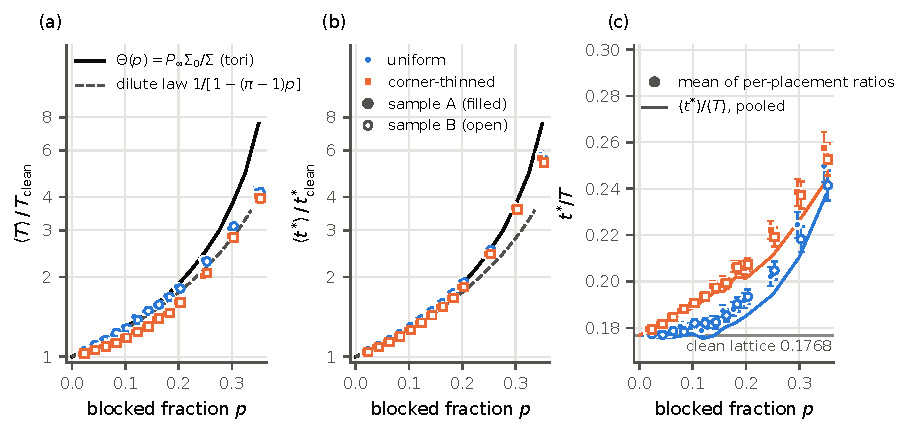
\includegraphics[width=\textwidth]{s7_defects_density_sweep.pdf}
% src: code/article/s7_defects_density_figures.py; data data/article/s7_defects_density_pooled.csv, data/msc_defects/homogenization.json
\caption{Density sweep, $N=35$, $q=0.8$, corner to opposite corner, discrete time. (a)~Mean and (b)~mode divided by
their clean values, and (c)~$\tmode/\MF$, against the blocked fraction $p$, for uniform placement (circles) and
corner-thinned placement (squares). Filled symbols: sample~A; open symbols: sample~B ($400$ placements each; bars are
$95\%$ intervals over placements; the samples are displaced horizontally for clarity). In (a) and (b) the solid curve
is the homogenised factor $\Thetap_{192}(p)$ measured on tori (Table~\ref{s7_defects_density:tab-homog}) and the dashed
curve the dilute law \eqref{s7_defects_density:eq-dilute} in the form $1/[1-(\pi-1)p]$. In (c) the symbols are means of
per-placement ratios and the lines the pooled ratio of ensemble means; the horizontal line is the clean value $0.1768$.}
\label{s7_defects_density:fig-sweep}
\end{figure}

\subsection{Effective medium and time dilation}\label{s7_defects_density:ssec-emt}

The walk with cancelled moves on a site-diluted lattice is the ``blind ant'' of the percolation literature
\citep{HavlinBenAvraham1987}. Its stationary distribution is uniform on the accessible cluster, and the Einstein relation
ties the long-distance diffusivity $\Deff$ to the conductivity $\cond$ of the network of unit resistors on the open
bonds: $\cond/\condz=\Pinf\,\Deff/\Dzero$, where $\Pinf$ is the fraction of sites in the accessible cluster
\citep{HavlinBenAvraham1987,StaufferAharony1994}. We define the time-dilation factor
\begin{equation}\label{s7_defects_density:eq-theta}
  \Thetap(p)=\frac{\Dzero}{\Deff(p)}=\Pinf(p)\,\frac{\condz}{\cond(p)} .
\end{equation}
The hypothesis to be tested is that, on scales large compared with the percolation correlation length, uniformly random
defects multiply every time scale by $\Thetap(p)$ and leave the shape of the first-passage law, hence $\ratio$, unchanged.
For the mean this is the coarse-grained form of \eqref{s7_defects_density:eq-resistance}. $\Thetap$ diverges at the blocked
fraction $p_{\mathrm c}=1-0.5927=0.4073$ \citep{NewmanZiff2000}.
% src: Newman and Ziff (2000): site-percolation threshold of the square lattice 0.59274621(13)

At small $p$ the conductivity follows from the response of a single blocked site. Let $\pk$ be the potential kernel of
the planar simple random walk \citep{Spitzer1976}, with $\pk(\mathbf 0)=0$, $\pk(\pm\ve_i)=1$ and $\pk(\pm2\ve_i)=4-8/\pi$.
% src: Spitzer1976 (potential kernel; values recomputed by quadrature in data/article/s7_defects_density_dipole_check.json: a10 = 1.0000000000000002, a20 = 1.4535209105296745 = 4 - 8/pi)

\begin{proposition}[Dipole response of one blocked site]\label{s7_defects_density:prop-dilute}
On the infinite square lattice with unit conductances, remove the site $\mathbf 0$ together with its four bonds and
impose the potential $-E x_1$ at infinity. Then:
(a) the potential is unique, $U(\vx)=-Ex_1-\frac{\pi E}{8}\,[\pk(\vx+\ve_1)-\pk(\vx-\ve_1)]$, and at the two neighbours
$\pm\ve_1$ of the removed site it is $\mp\pi E/2$ (instead of $\mp E$);
(b) the removed site lowers the dissipated power by $\pi E^{2}$, in the sense that $\sum_{b}U^{0}_{b}U_{b}=\pi E^{2}$ over
the four removed bonds, and in every finite network of unit resistors with prescribed boundary potentials removing a
set of bonds lowers the dissipated power by exactly $\sum_{b\ \mathrm{removed}}U^{0}_{b}U_{b}$.
\end{proposition}

\begin{heuristic}[Dilute law]\label{s7_defects_density:res-dilute}
For uniformly placed blocked sites on the square lattice, as $p\to0$,
\begin{equation}\label{s7_defects_density:eq-dilute}
  \frac{\cond}{\condz}=1-\pi p+\Order(p^{2}),\qquad
  \frac{\Deff}{\Dzero}=1-(\pi-1)\,p+\Order(p^{2}),\qquad
  \Thetap(p)=1+(\pi-1)\,p+\Order(p^{2}).
\end{equation}
\end{heuristic}

The derivation treats each blocked site as isolated in the unperturbed field (Proposition~\ref{s7_defects_density:prop-dilute}
and $\Pinf=1-p+\Order(p^{4})$); the step from one defect to a density of defects is not proved here, hence the label. The
law is not new: \citet{WatsonLeath1974} gave $\cond/\condz=1-\pi p+\tfrac12\pi p^{2}$ from an effective-medium theory, and
\citet{Nieuwenhuizen1986} calculated the diffusion coefficient and conductivity of exactly this walk to order $p^{2}$, with
the coefficients printed in \citet{Ernst1987}:
\begin{equation}\label{s7_defects_density:eq-second-order}
  \frac{\cond}{\condz}=1-\pi p+1.2858\,p^{2}+\cdots,\qquad
  \frac{\Deff}{\Dzero}=1-(\pi-1)\,p-0.8558\,p^{2}+\cdots .
\end{equation}
Our own evaluation of the pair term on tori gives $1.28588$ and $-0.85571$, within $10^{-4}$ of the printed values, and
the conductivities measured on $192\times192$ tori agree with \eqref{s7_defects_density:eq-second-order} to $6.2\times10^{-4}$ for
$p\le0.18$; the estimates $\Thetap_{192}$ of the time-dilation factor are $1.045$, $1.289$, $1.877$ and $3.739$ at $p=0.02$, $0.1$,
$0.2$ and $0.3$ (Supplementary Table~\ref{s7_defects_density:tab-homog}).
% src: data/article/s7_defects_density_second_order.json (a2_extrapolated_linear_in_Nt^-2_last3, D2_coefficient_from_extrapolated_a2, extrapolated_minus_published); data/article/derived_checks.json (E_dilute_laws: max_abs_sigma_minus_exact_second_order_p_le_0.18); data/msc_defects/homogenization.json (finite_p); coefficients 1.2858 and -0.8558: Ernst, Nieuwenhuizen and van Velthoven (1987), Eqs (4.2), (4.3)

\emph{Test at $N=35$.} Under uniform placement and $p\le0.2$ the pooled factor of the mean is within $2.8\%$ of
$\Thetap_{192}(p)$ and that of the mode within $1.82\%$, with no fitted parameter (Fig.~\ref{s7_defects_density:fig-sweep}(a,b));
these are ensemble-mean estimates, whose $95\%$ intervals reach $\pm1.8\%$ for the mean and $\pm0.72\%$ for the mode
(relative to $\Thetap_{192}$), so that the deviations of the mean are of the size of their sampling uncertainty.
For $p\ge0.25$ the mean falls below $\Thetap$ ($3.08$ against $3.74$ at $p=0.3$) while the mode still follows it ($3.66$);
those densities describe a selected ensemble on a lattice not much larger than the correlation length. The simplest
mean-field description of defects, a reduced activity $q_{\mathrm{eff}}(p)$, cannot capture the changes of $\ratio$ found
below: a change of activity only rescales time, and by \eqref{s2_model:eq-qscaling} and
Proposition~\ref{s2_model:prop-structure}(d) it leaves $\ratio$ unchanged up to a few steps
(Section~\ref{s6_mechanism:sec}).
% src: data/article/s7_defects_density_pooled.json (statements.uniform_max_abs_mfpt_fac_over_theta_pct_p_le_0.20_pooled, uniform_max_abs_mode_fac_over_theta_pct_p_le_0.20_pooled); data/article/s7_defects_density_pooled.csv (uniform, p <= 0.20: mfpt_fac_ci_P / theta_L192 up to 1.77 %, mode_fac_ci_P / theta_L192 up to 0.719 %)

\emph{Larger lattices.} For uniform placement at $p=0.1$ and $0.2$ we computed modes up to $N=200$, certified by
Proposition~\ref{s3_methods:prop-certificate} in double precision, and means up to $N=280$, with the most precise estimates $\Thetap_{200}(0.1)=1.2877$ and $\Thetap_{200}(0.2)=1.8783$. The mode factor equals
$\Thetap$ to within $1.11\%$ at $p=0.1$ and $1.6\%$ at $p=0.2$ for every $N$ from $15$ to $200$; the factor of the mean divided by
$\Thetap$, averaged over $N=35$--$280$, is $1.004\pm0.005$ and $0.987\pm0.007$. The shift of $\langle\tmode/\MF\rangle$ relative
to the clean lattice of the same size is between $+0.6\%$ and $+1.2\%$ for $N\ge50$ at $p=0.1$; at $p=0.2$ it falls from
$+9.4\pm1.8\%$ at $N=35$ (in the $400$ placements of this size study; the $800$ pooled placements of Section~\ref{s7_defects_density:ssec-sweep} give $+8.9\%$) to $+4.5\pm1.4\%$ at $N=100$ and $+3.9\pm2.7\%$ at $N=200$: it halves but is not shown to vanish
(Supplementary Table~\ref{s7_defects_density:tab-size}). A slow approach is to be expected, because in
\eqref{s7_defects_density:eq-resistance} the constant that accompanies $\ln N$ in $\Glap_{\va\va}$ is set by the immediate
surroundings of the target.
% src: data/article/s7_defects_density_pooled.json (size_dependence.summary); data/msc_defects_verify/v07_summary.csv, v07b_summary.csv, v04b_theta.json

\begin{conjecture}[Homogenisation]\label{s7_defects_density:conj-homog}
Fix $p<p_{\mathrm c}$ and place $\mathrm{round}(pN^{2})$ blocked sites uniformly, conditioned on $\va\in\Cset$. As
$N\to\infty$, $\langle\MF\rangle/(\Thetap(p)\,\MF_{\mathrm{clean}})\to1$ and
$\langle\tmode\rangle/(\Thetap(p)\,\tmode_{\mathrm{clean}})\to1$, so that $\langle\tmode\rangle/\langle\MF\rangle$ divided by the
clean ratio at the same $N$ tends to one.
\end{conjecture}

\subsection{Placement decides the direction}\label{s8_defects_placement:ssec-capture}

By \eqref{s7_defects_density:eq-resistance}, $\MF=(4\nn/q)(\Glap_{\va\va}-\Glap_{\vo\va})$. The rows of $\Glap$ sum to zero, so
$(4\nn/q)\,\Glap_{\va\va}$ is the mean first-passage time from a uniformly distributed start, and the actual start enters
only through the cross term $\Glap_{\vo\va}$ ($-0.221$ against $\Glap_{\va\va}=2.082$ on the clean lattice). We call
$\Glap_{\va\va}$ the \emph{capture resistance} of the target. It controls the mean: over the 400 uniform placements at
$p=0.1$ and at $p=0.2$ the rank correlation between $\MF$ and $\Glap_{\va\va}$ is $0.9995$ and $0.9986$ (sample~A; $0.9995$ and
$0.9982$ in sample~B), whereas that between $\MF$ and the number of blocked sites near the start is below $0.08$ in
absolute value; and at $p=0.2$ the uniform and the corner-thinned placements leave the same accessible volume
($\nn/N^{2}=0.797$) but raise $\Glap_{\va\va}-\Glap_{\vo\va}$ by the factors $2.310$ and $2.022$.
% src: data/msc_defects/structured_deterministic.csv (row clean: G_tt, G_st); data/msc_defects/summary_correlations.csv (G_tt, blk_s_r3, blk_s_r6); data/msc_defects_verify/v09_mechanism.json (G_aa, blk_s6); data/msc_defects/summary_sweep_N35.csv (n_factor, Gdiff_factor)
The mode responds to a different part of the lattice. Blocking a single site shortens the mean for $67.6\%$ of the sites
(the lost volume), and the positive responses are concentrated around the target, where $64\%$ of $\sum_{\vx}\chiT(\vx)$ comes
from sites within distance 3; the response of the mode is spread over the whole region between start and target
($19\%$ within distance 3 of the target), and only $5.4\%$ of the sites lower it
(Fig.~\ref{s8_defects_placement:fig-maps}).
% src: data/msc_defects/summary_first_order.json; data/msc_defects_verify/v05_sens_N35.json; data/article/s8_defects_placement_checks.json (susceptibility_N35)

\begin{table}[tbp]
\centering
\caption{Localised random placements of $M$ blocked sites ($N=35$, $q=0.8$, 200 placements per row and sample,
mean $\pm$ 95\% confidence interval). Factors are relative to the clean lattice, for which $\tmode/\MF=0.1768$.}
\label{s8_defects_placement:tab-local}
\small
\begin{tabular}{lrcccc}
\toprule
 & & \multicolumn{3}{c}{sample A} & sample B\\
\cmidrule(lr){3-5}\cmidrule(lr){6-6}
region & $M$ & $\MF$ factor & $\tmode$ factor & $\tmode/\MF$ & $\tmode/\MF$\\
\midrule
anywhere    & 40 & $1.086\pm0.017$   & $1.080\pm0.005$ & $0.1771\pm0.0016$ & $0.1780\pm0.0016$\\
centre      & 40 & $1.0086\pm0.0008$ & $1.150\pm0.003$ & $0.2015\pm0.0004$ & $0.2014\pm0.0004$\\
near start  & 10 & $0.9933\pm0.0001$ & $1.012\pm0.001$ & $0.1801\pm0.0001$ & $0.1802\pm0.0002$\\
near start  & 40 & $0.999\pm0.003$   & $1.320\pm0.027$ & $0.2329\pm0.0040$ & $0.2368\pm0.0048$\\
near target & 10 & $1.239\pm0.029$   & $1.056\pm0.006$ & $0.1530\pm0.0020$ & $0.1530\pm0.0019$\\
near target & 20 & $1.659\pm0.057$   & $1.134\pm0.009$ & $0.1249\pm0.0024$ & $0.1276\pm0.0025$\\
near target & 30 & $2.281\pm0.083$   & $1.230\pm0.011$ & $0.0994\pm0.0023$ & $0.0991\pm0.0024$\\
near target & 40 & $3.367\pm0.127$   & $1.357\pm0.015$ & $0.0752\pm0.0022$ & $0.0741\pm0.0021$\\
\bottomrule
\end{tabular}
% src: data/msc_defects/summary_structured_local.csv (sample A); data/msc_defects_verify/v06_local.csv via data/article/s8_defects_placement_checks.json (local_sample_B)
\end{table}

To separate placement from density we block $M$ sites drawn uniformly inside one region: within Euclidean distance 12 of
the target (122 candidate sites), within distance 12 of the start (122 sites), within $6.2$ of the centre (121 sites), or
anywhere (Table~\ref{s8_defects_placement:tab-local}, Fig.~\ref{s8_defects_placement:fig-structured}). Forty blocked sites,
$3.3\%$ of the lattice, multiply the mean by $3.37\pm0.13$ and the mode by $1.36$ near the target, so that the ratio falls to
$0.0752\pm0.0022$, less than half its clean value; near the start they leave the mean unchanged ($\times0.999\pm0.003$),
delay the mode by a third and raise the ratio to $0.2329\pm0.0040$. Deterministic obstacles behave in the same way: serpentine
corridors push the law towards the one-dimensional shape ($\tmode/\MF=0.316$--$0.339$), walls between start and target
raise the ratio to between $0.244$ and $0.328$, whereas a wall next to the target lowers it to $0.135$; enclosing the
target makes the law more nearly exponential (ratio $0.0925$ for ten blocked sites), and a solid $12\times12$ block in the centre
\emph{lowers} the mean by $4.6\%$ and delays the mode by $23\%$. Hence $\tmode/\MF$ is not a function of the defect density:
it decreases when the defects surround the target, increases when they lie around the start or between start and target,
and, when they are spread uniformly, stays within a few per cent of its clean value at low density ($p\le0.14$;
Section~\ref{s7_defects_density:ssec-sweep}) but rises by
$4.7\%$ to $8.9\%$, depending on the estimator, at $p=0.2$.
% src: data/article/s7_defects_density_pooled.json (statements.uniform_ratio_excess_pct_by_p, uniform_rom_excess_pct_by_p: p = 0.14 and 0.20)
% src: data/msc_defects/summary_structured_local.csv (mfpt_factor, mode_factor, ratio); data/msc_defects/structured_deterministic.csv via data/article/s8_defects_placement_checks.json (deterministic, deterministic.block12_centre)

\begin{figure}[tbp]
\centering
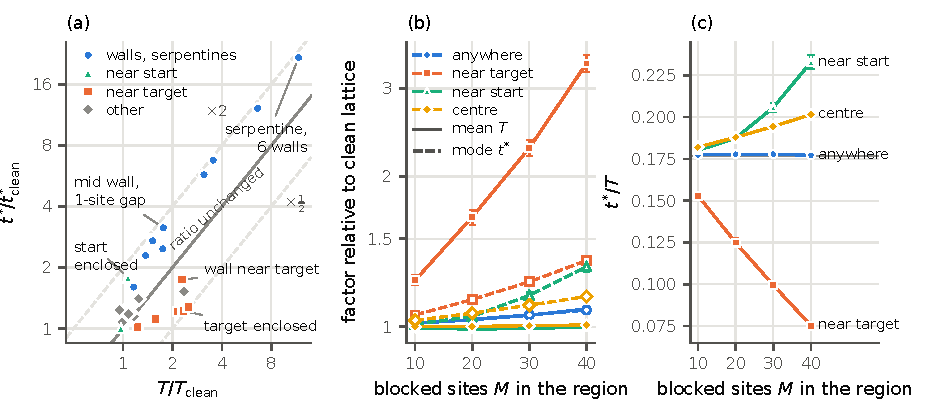
\includegraphics[width=\textwidth]{s8_defects_placement_structured.pdf}
\caption{Placement decides the direction ($N=35$, $q=0.8$, corner to opposite corner, discrete time).
(a)~Mode factor against mean factor for the 28 deterministic geometries of
Table~\ref{appC_tables:tab-deterministic}, logarithmic axes; on the solid line $\tmode/\MF$ keeps its clean value,
on the dashed lines it is doubled or halved. (b)~Mean (solid lines) and mode (dashed lines) relative to the clean
lattice for $M$ blocked sites drawn inside a region. (c)~The resulting ratio; the grey line is the clean value.
In (b) and (c) the points are means over the 200 placements of sample~A and the bars 95\% confidence intervals.}
% src: data/msc_defects/structured_deterministic.csv, summary_structured_local.csv (figure: code/article/s7s8_defects_figures.py, fig_structured)
\label{s8_defects_placement:fig-structured}
\end{figure}

\emph{Two time scales.} Beyond the transit time the PMF is dominated by its two slowest terms, with time constants
$\Tcap=-1/\ln(1-q\nu_0)$ (the capture time) and $\tau_1=-1/\ln(1-q\nu_1)$; with $1/\tau=1/\tau_1-1/\Tcap$ and
$c=-b_1/b_0$, the maximiser of the two-term sum is $\tmode\approx\tau\ln[c(1+\Tcap/\tau)]$. A pure dilation multiplies $\Tcap$
and $\tau$ by the same factor and leaves $\tmode/\MF$ unchanged, whereas a perturbation that raises only the capture time
moves the mode sub-linearly: on the clean lattice the exponent $\partial\ln\tmode/\partial\ln\Tcap$ is $0.21$ with $\tau$
and $c$ held fixed, and $0.17$ with $\tau_1$ and $c$ held fixed ($\tau$ then follows $\Tcap$). The exact
elasticities $\ln(\tmode\ \text{factor})/\ln(\MF\ \text{factor})$ of obstacles that enclose the target are somewhat larger,
$0.234$ to $0.310$, and the regression of $\ln\tmode$ on $\ln\MF$ across the uniform placements at $p=0.2$ has slope $0.30$. This
heuristic accounts for the sign and the approximate size of the effect and has no controlled error; it fails for a wall
near the target, which also lengthens the transit (Supplementary Section~\ref{sup_defects:ssec-twotime}).
% src: data/article/s8_defects_placement_checks.json (two_time.elasticity_formula, two_time.elasticity_formula_tau1_c_fixed, two_time.cross_placement_slope_p02); data/msc_defects_verify/v09b_twotime.csv (elasticity_exact); data/msc_defects_verify/v09_mechanism.json (p0.20.loglog_slope_mode_on_mfpt)

\emph{A one-parameter family of shapes.} Over all $13\,631$ exactly solved configurations of sample~A the coefficient of
variation is nearly a function of $\ratio$ alone (Pearson correlation $-0.981$; a quadratic fits with a root-mean-square
residual of $0.0045$); sample~B gives $-0.983$. We record this as an empirical regularity, without a theory: size, density
and placement appear to act mainly by moving the law along one line between a transit-limited shape and a
capture-limited, nearly exponential one.
% src: data/article/s8_defects_placement_checks.json (shape_family.sample_A); data/msc_defects_verify/v09_mechanism.json (family_main_implementation, family_recheck)

\emph{Other defect types.} On a chain, a barrier crossed with reduced probability costs more the nearer it is to the target
(Proposition~\ref{s8_defects_placement:prop-1d-barriers}; for a single barrier this is Eq.~(12) of
\citet{SarvaharmanGiuggioli2023}, who also showed that a barrier behind the start changes the mode and the tail but not
the mean, their `disorder indifference'), and uniformly random barriers are again a dilation of time. On the
square lattice, permeable obstacles at $p=0.1$ leave the ratio within $3.2\%$ of its clean value, but the limit of vanishing
permeability is singular, because a site that can be entered at all carries its full share of the stationary distribution.
Partial traps, which remove the walker with probability $\trap$ per step, remove the long trajectories and act in the
opposite sense to obstacles: the ratio of mode to conditional mean rises from $0.178$ to $0.638$ as $\trap$ grows from $10^{-5}$
to $10^{-2}$ at $p=0.1$ (Supplementary Section~\ref{sup_defects:ssec-other}).
% src: data/msc_defects/summary_beyond.json (2d_permeable, 2d_traps); data/msc_defects_verify/v08_beyond.json (perm, traps); data/article/s8_defects_placement_checks.json (permeable)

Within this model, and at the sizes computed, the mean and the mode respond to different parts of the lattice: the mean
to the capture resistance of the target, which is set by its immediate surroundings, and the mode to the transit between
start and target. We make no claim beyond the lattices, sizes and defect models examined here.

% s9_discussion.tex -- Discussion and conclusions.
% This section introduces NO new numbers.  Every number below is quoted from an earlier section and carries the
% same "% src:" comment (paths relative to the root of the repository).
\section{Discussion and conclusions}\label{s9_discussion:sec}

\subsection{What is established, and with what status}\label{s9_discussion:ssec-status}

The results of this article do not all have the same standing; Table~\ref{s9_discussion:tab-status} sorts them.
``Exact numerics'' are computations that are exact in the sense of Section~\ref{s3_methods:sec} (up to double-precision
round-off for time stepping, to a measured accuracy for Laplace inversion) and cross-checked by separately written routes and
implementations; they hold at the sizes run and are not theorems. The proofs of
Section~\ref{s6b_rigorous:sec} were checked within this project (Section~\ref{s6b_rigorous:ssec-status}), not by external
referees.

{\small
\begin{longtable}{@{}p{2.4cm}p{10.6cm}p{2.1cm}@{}}
\caption{Status of the main statements. Discrete-time values are for $q=0.8$; defect results are for $\dd=2$
with a corner start and the opposite corner as target.}
\label{s9_discussion:tab-status}\\
\toprule
Status & Statements & Where \tabularnewline
\midrule
\endfirsthead
\toprule
Status & Statements & Where \tabularnewline
\midrule
\endhead
Proved &
Exact structure, interlacing, pseudo-inverse formula; cosine sum in any dimension; single sums for $\dd=2$ and every
$N\ge2$; $q\TN=2N^{2}\Reff_N$; double sum for $\dd=3$; the large-$N$ expansion; certificate of the global mode; the limit
$\tmode/\MF\to2\xi^{*}$ on the chain in continuous time and for $q\le\tfrac12$; factorisation of the renewal ratio;
unimodality of the three point-target placements in continuous time and for $q\le1/(1+\cos\frac\pi N)$; signs of the
residues (their non-alternation for $\dd\ge2$, $N\ge3$ provisional, \lateproof); bounds on the slowest pole; failure of unimodality near $q=1$ on the chain; resistance identity and dipole
response with blocked sites.
& \raggedright Secs.~\ref{s2_model:sec}--\ref{s7_defects:sec} \tabularnewline
\addlinespace
\raggedright Proved with computer assistance &
Unimodality for $q\le\frac45$ from corner to corner (for the centre placements when $\dd\ge2$; a threshold attained on
the chain with $N=4$), and on finite ranges beyond: up to $q=1$ for $\dd=3$ ($N\le30$), $\dd=4$ ($N\le8$) and $\dd=5$
($N\le5$), and $q\le\frac{499}{500}$ for $\dd=2$ ($N\le64$). In one
dimension $\tmode/\MF\to0.33328426549\ldots$ for every $q$, with windows of width about one step for $q\le\frac45$. For
corner-to-corner transport in $\dd=2,3$: the scaled error of the closed form \eqref{s6_mechanism:eq-L1-simple} bounded
for every $N\ge12$ ($\dd=2$) and $N\ge10$ ($\dd=3$), and the leading laws with explicit remainders, in continuous time
and, in discrete time, for $q\le0.99$ once $N\ge N_0$ and, provisionally (\lateproof), for every $q<1$ once
$N\ge\max(N_0,N_1(q))$; exact modes on finite ranges, the closed form within $0.971\%$ ($\dd=2$) and $0.275\%$ ($\dd=3$)
there for $q\in\{\frac45,\frac12\}$ and $N\ge10$, and within $0.3\%$ in three dimensions for $q\in\{\frac45,\frac12\}$
and every $N\ge10$. Means: a remainder for every $N$ ($\dd=2$); $\Kthree$,
$\Kthreep$ and the next constant ($\dd=3$).
% src: data/msc_rigorous_1d/03_constants.json; data/msc_rigorous_certified/closedform_summary_c128.json; data/article/s6b_rigorous_checks.json
& \raggedright Secs.~\ref{s4_mfpt:sec}, \ref{s6b_rigorous:sec} \tabularnewline
\addlinespace
\raggedright Exact numerics at the stated sizes &
Distributions and modes in discrete time up to $N=1000$, $401$, $100$ ($\dd=1,2,3$), each mode a certified global
maximiser (in exact arithmetic or with an a-priori bound on round-off), and in continuous time up to $N=1.7\times10^{7}$ ($\dd=2$) and $N=4096$ ($\dd=3$); for $\dd=2$, $\tmode/\MF$
falling from $0.27$ ($N=5$) to $0.056$ ($N=1.7\times10^{7}$), for $\dd=3$ from $0.153$ ($N=5$) to $0.0118$ ($N=100$) and
$4.1\times10^{-4}$ ($N=4096$, continuous time); the
expression of $\Kthreep$ through $\xiH$ and $\varkappa$; all defect statistics, up to placement sampling error: under
uniform placement $\tmode/\MF$ within $3.3\%$ of its clean value $0.1768$ up to $p=0.14$, and at $p=0.2$ the mean of
the per-placement ratios $8.9\%$ above it (the ratio of ensemble means $4.7\%$); forty blocked sites near the target give
$0.075$, near the start $0.233$; the coefficient of variation is nearly a function of $\tmode/\MF$ (an empirical
regularity).
% src: data/msc_modes/discrete_modes.jsonl; data/msc_modes/laplace_modes.jsonl; data/article/s3_methods_certificate.json; data/msc_modes/tables.md (T2, T3); data/msc_modes/summary_tables.md (M2); data/article/s6b_rigorous_checks.json (d3_constants); data/article/s7_defects_density_pooled.json (statements.uniform_ratio_excess_pct_by_p, uniform_rom_excess_pct_by_p); data/msc_defects/summary_structured_local.csv; data/article/s8_defects_placement_checks.json (shape_family.sample_A)
& \raggedright Secs.~\ref{s3_methods:sec}--\ref{s7_defects:sec} \tabularnewline
\addlinespace
\raggedright Formal asymptotics &
Closed-form approximation \eqref{s6_mechanism:eq-L1} for placements other than corner to corner (corner to centre:
within $0.964\%$ for $\dd=2$ and $0.206\%$ for $\dd=3$ at the computed sizes); dilute law \eqref{s7_defects_density:eq-dilute};
first-order susceptibility estimate.
% src: data/article/closed_form_checks.json (2d_C2M, 3d_C2M)
& \raggedright Secs.~\ref{s6_mechanism:sec}, \ref{s7_defects:sec} \tabularnewline
\addlinespace
Heuristic &
Two-time-scale account of the sub-linear response of the mode to a change of capture time.
& Sec.~\ref{s7_defects:sec} \tabularnewline
\addlinespace
Conjecture &
Time dilation by $\Thetap(p)$ exact as $N\to\infty$; the closed form within $1\%$ in two dimensions for every $N\ge10$;
the mode laws at $q=1$; unimodality for $\frac45<q<1$ and every $N$; log-concavity for $\dd\ge2$.
& \raggedright Secs.~\ref{s6b_rigorous:sec}, \ref{s7_defects:sec} \tabularnewline
\addlinespace
Refuted &
Alternating residues for opposite corners in $\dd\ge2$; unimodality of every point-target law; the closed form in one
dimension (on the certified ranges with $N\ge10$ at $q=\frac45$ it overestimates the mode by at least $15.77\%$ and at
most $22.51\%$).
% src: data/msc_rigorous_certified/closedform_summary_c128.json (d1_q4-5); data/msc_rigorous_1d/39_hand_constants.json
& Sec.~\ref{s6b_rigorous:sec} \tabularnewline
\bottomrule
\end{longtable}}

\subsection{The physical picture}\label{s9_discussion:ssec-picture}

Two times govern the problem. The mean is a capture time: a walker that has spread over the box finds the target at a
rate fixed by the number of sites times the capture resistance of the target, \eqref{s2_model:eq-resistance}, which gives
$N^{2}$, $N^{2}\ln N$ and $N^{3}$ for $\dd=1,2,3$. The mode is a relaxation time: the first-passage density peaks when the
transient of arrival across the box, which decays at a rate $\mu\propto N^{-2}$ in every dimension, has fallen to the level
of the slow capture decay, and this costs only the logarithmic factor $\ln(AX)$ of \eqref{s6_mechanism:eq-L1}, where
$X=\mu\,q\MF$ measures how weak a sink the target is. For corner-to-corner transport in two and three dimensions this
picture is a theorem (Section~\ref{s6b_rigorous:ssec-cf}); in one dimension $X$ stays bounded and the two times are of the
same order. Hence the dimension dependence of Table~\ref{s5_modes:tab-laws}: $\tmode/\MF$ tends to a constant for $\dd=1$,
falls slowly for $\dd=2$ and quickly for $\dd=3$, and the separation between mean and mode grows with dimension. For a
point target in $\dd\ge2$ the law is close to an exponential preceded by a short dead time, and the mode marks the end of
that dead time: it is not a typical time. The appropriate typical value is the median, about $0.7\,\MF$, and statements
about waiting times must be made with the survival function $\Sv(t)$, not with $\tmode/\MF$.
% src: data/msc_modes/medians.json

The same two times organise the defect results. Uniformly placed blocked sites slow capture and relaxation by nearly the
same factor $\Thetap(p)$, so that $\tmode/\MF$ stays near its clean value at low density; the rise at $p=0.2$ shrinks with $N$
but is not shown to vanish. Blocked sites around the target raise the capture resistance, hence the mean, far more than
the mode; blocked sites around the start or between start and target delay the transit, hence the mode, and leave the
mean almost unchanged.

\subsection{Relation to the literature}\label{s9_discussion:ssec-literature}

By the commute-time identity the two-dimensional results on the mean are statements about the resistor grid, and in that
form they were already published \citep{CondaminBenichou2006,Wu2004,Giuggioli2020,EssamWu2009,IzmailianHuang2010,TanTan2020};
we add a self-contained proof in the random-walk setting for both parities of $N$ and record the overflow-free form
\eqref{s4_mfpt:eq-single-S}, an elementary rearrangement. The shape of the law
agrees with the picture of geometry-controlled kinetics in confined domains
\citep{Benichou2010,Meyer2011,BenichouVoituriez2014,Mattos2012,GodecMetzler2016,Grebenkov2018} and with the exponential
approximation of hitting times for reversible chains \citep{AldousBrown1992}; we add exact lattice distributions and modes
and their explicit dependence on $N$ and $\dd$; the most probable time of direct trajectories and the relation of the
median to the mean are given by \citet{GodecMetzler2016} and \citet{Grebenkov2018}. Apart from their classical
ingredients (the interlacing of relaxation and first-passage spectra \citep{HartichGodec2018,HartichGodec2019}, the
mixture and exponential laws from the uniform and the quasi-stationary start \citep{AldousFill}, unimodality on the chain
in continuous time \citep{Keilson1971}), we have not found in print the theorems of Section~\ref{s6b_rigorous:sec} on
the mode of a lattice first-passage time, the explicit closed-form approximation \eqref{s6_mechanism:eq-L1}, whose ingredients are the
lattice counterpart of known small-target asymptotics \citep{WardKeller1993,IsaacsonNewby2013}, or the expressions
\eqref{s4_mfpt:eq-coeffs} through the lemniscate constant, which specialise the general expressions of
\citet{IzmailianHuang2010}. Our search was targeted, not exhaustive, and we claim no priority. The dilute law for blocked
sites is in the literature \citep{WatsonLeath1974,Nieuwenhuizen1986,Ernst1987}, and our measured conductivities agree with
its published second-order form. That the placement of a defect decides whether the mean or only the mode and the tail
respond was shown by \citet{SarvaharmanGiuggioli2023} for a single barrier on a chain (their Eq.~(12) is our
Proposition~\ref{s8_defects_placement:prop-1d-barriers} for one barrier); Section~\ref{s7_defects:sec} adds the exact
two-dimensional ensembles of blocked sites.

\subsection{Limitations}\label{s9_discussion:ssec-limitations}

\begin{enumerate}
\item Unimodality is proved for the three point-target placements studied here in continuous time, and in discrete
time for $q\le\frac45$ from corner to corner (for the centre placements when $\dd\ge2$), and on finite ranges beyond;
two computed runs at $q=0.9$ lie outside the proved ranges of unimodality, and the 16 computed corner-to-corner runs at
$q=0.3$ and $0.9$ lie outside the certified ranges of the mode and rest on the a-priori round-off bound of
Section~\ref{s3_methods:sec}. The
continuous-time modes at sizes beyond time stepping are global maximisers by Theorem~\ref{s6b_rigorous:thm-unimodal}, but
their location rests on numerical Laplace inversion, to the accuracy of Table~\ref{s3_methods:tab-validation}, not on a
certificate.
\item The closed form is proved only for corner-to-corner transport in $\dd=2,3$, with a window a few units wide in
$X\muone(\tmodec-q\tcf)$. In two dimensions its $1\%$ accuracy is proved only on finite ranges and for very large $N$, and
the asymptote $N^{2}\ln\ln N$, although proved, is not reached by the data.
\item The computer-assisted proofs rest on their trusted bases (Python integers; Arb ball arithmetic through
python-flint together with the transcription of the formulas into the scripts; beyond the Python-integer ranges, a C
program run twice, which is the only witness for 2242 of its 3824 certificates). No program was verified in a proof
assistant, the certificate of Theorem~\ref{s6b_rigorous:thm-disc}(c) has not been re-run by separately written code, and
all proofs were checked within this project, not by external referees; the statements marked \lateproof{} are
provisional until examined by a reader outside the project.
% src: proofs/R0_rigorous_results/R0_rigorous_results.tex (Section 9: trusted bases; separately written re-checks)
\item The expression of $\Kthreep$ through $\xiH$ and $\varkappa$ is identified numerically and is unproved.
\item Only four placements were studied (corner to corner, corner to centre, centre to corner, and exit through an
absorbing boundary layer); \eqref{s6_mechanism:eq-L1} does not apply to the third.
\item Inert defects were studied only for $\dd=2$, a corner target and $q=0.8$, up to $N=280$ for means and $N=200$ for
modes; barriers on the chain only at $N=100$. A corner target has two neighbours, which makes the mean unusually
sensitive to its surroundings. Placements are conditioned on start and target being connected; for $p\ge0.3$ at $N=35$
the results describe a selected, near-critical ensemble, not bulk properties.
% src: data/msc_defects_verify/v07_summary.csv, v07b_summary.csv; data/msc_defects/summary_sweep_N35.csv (acceptance)
\item Time dilation by $\Thetap(p)$ is accurate at $p=0.1$ and a $1$--$3\%$ approximation at $p=0.2$ at the sizes computed;
its exactness as $N\to\infty$ is a conjecture. The model is a lattice walk with a single walker.
\end{enumerate}

\subsection{Open problems}\label{s9_discussion:ssec-open}

(a) Unimodality for $\frac45<q<1$ and every $N$, and log-concavity of the law for $\dd\ge2$. (b) Sharp constants for the
closed form: $N$-dependent window constants sharp enough to close the gap $302\le N<1\,761\,450$ of
Conjecture~\ref{s6b_rigorous:conj-cf}(a), the value of the limit of $X\muone(\tmodec-q\tcf)$, and the discrete walk close
to $q=1$. (c) The mode for a general start and target, including placements for
which the slowest target-visible mode does not have a positive amplitude $A$. (d) A proof of the expression of $\Kthreep$
through $\xiH$ and $\varkappa$, and whether the series \eqref{s4_mfpt:eq-expansion} diverges. (e) Defects in three
dimensions and around interior targets, and the large-$N$ behaviour under uniform placement
(Conjecture~\ref{s7_defects_density:conj-homog}).

\subsection{Conclusions}\label{s9_discussion:ssec-conclusions}

For a lazy walk in a reflecting box with one absorbing site the mean first-passage time is given by exact finite sums
and is equivalent, in two dimensions, to a resistance that was already in the literature. The most probable
first-passage time obeys a different law: it follows the relaxation time of the box, not the capture time, and it
separates from the mean more strongly as the dimension increases. For corner-to-corner transport this is proved, partly
with computer assistance: the law is unimodal in continuous time and, in discrete time, for $q\le\frac45$, while
unimodality fails near $q=1$ on the chain and, at $q=1$, at some sizes in two dimensions; in two and three dimensions
its mode follows a parameter-free closed form with a bounded scaled error, and the leading laws $N^{2}\ln\ln N$ and
$N^{2}\ln N$ hold with explicit remainders, in continuous time and, in discrete time, for $q\le0.99$ and, provisionally,
for every $q<1$ once $N$ is large enough; in one dimension $\tmode/\MF$ tends to $0.33328$ for every activity.
% src: data/msc_rigorous_1d/03_constants.json (c_mid_80_digits)
In the square-lattice setting studied here (corner target, mainly $N=35$), the direction
in which inert defects move the ratio of the two times is set by where they sit, not by how many there are.


% ------------------------------------------------------------------ end matter
\section*{Data and code availability}
All code and data needed to reproduce every number, table and figure of this article and of its Supplementary
Material are in the repository \citep{ZhouyiRepo}
\begin{center}\url{https://github.com/zhouyi-xiaoxiao/master-dissertation},\end{center}
together with the \LaTeX{} sources and a file \texttt{reproduce.md} that lists the exact commands. The folder
\texttt{proofs/} contains the companion notes R0--R5 \citep{NoteR0,NoteR1,NoteR2,NoteR3,NoteR4,NoteR5} with the
complete proofs of the results of Sections~\ref{s4_mfpt:sec} and~\ref{s6b_rigorous:sec}; the certificates of the computer-assisted proofs and the programs that check them are
in \texttt{data/msc\_rigorous\_*} and \texttt{code/msc\_rigorous\_*}. All computations are deterministic or use fixed
random seeds. The code of the internal checks of the proofs (counter-example searches and separately written
re-checks, Section~\ref{s6b_rigorous:ssec-status}) is not part of the repository.

\section*{Acknowledgements}
This article develops work begun in the author's MSc dissertation (University of Bristol, 2025).

\bibliographystyle{plainnat}
\bibliography{refs}

\end{document}
